\documentclass[a4paper,12pt]{article}
\usepackage{amsmath, bm}
\usepackage{amssymb,amsthm,graphicx}
\usepackage{enumitem}
\usepackage{color}
\usepackage{float}
\usepackage[mathscr]{euscript}
\usepackage{dsfont}
\usepackage{natbib}
\usepackage{amsmath}
\makeatletter
\renewcommand{\eqref}[1]{\tagform@{\ref{#1}}}
\def\maketag@@@#1{\hbox{#1}}
\makeatother
\usepackage{bibentry}
\usepackage[left=2.7cm,right=2.7cm,bottom=2.7cm,top=2.7cm]{geometry}
%\parindent0pt 
\newcommand{\doublehat}[1]{\skew{5.5}\widehat{\widehat{#1}}}
\newcommand{\doublehattwo}[1]{\widehat{\widehat{#1}}}
\newcommand{\gaussianstat}{\Phi^\prime}
\newcommand{\gaussiankernel}{\phi^\prime}
\newcommand{\pseudogaussianstat}{\Phi}
\newcommand{\pseudogaussiankernel}{\phi}




% General

\newcommand{\reals}{\mathbb{R}}
\newcommand{\integers}{\mathbb{Z}}
\newcommand{\naturals}{\mathbb{N}}

\newcommand{\pr}{\mathbb{P}}        % probability
\newcommand{\ex}{\mathbb{E}}        % expectation
\newcommand{\var}{\textnormal{Var}} % variance
\newcommand{\cov}{\textnormal{Cov}} % covariance

\newcommand{\law}{\mathcal{L}} % law of X
\newcommand{\normal}{N}        % normal distribution 

\newcommand{\argmax}{\textnormal{argmax}}
\newcommand{\argmin}{\textnormal{argmin}}

\newcommand{\ind}{\mathbbm{1}} % indicator function
\newcommand{\kernel}{K} % kernel function
\newcommand{\wght}{W} % kernel weight
\newcommand{\thres}{\pi} % threshold parameter


% Convergence

\newcommand{\convd}{\stackrel{d}{\longrightarrow}}              % convergence in distribution
\newcommand{\convp}{\stackrel{P}{\longrightarrow}}              % convergence in probability
\newcommand{\convas}{\stackrel{\textrm{a.s.}}{\longrightarrow}} % convergence almost surely
\newcommand{\convw}{\rightsquigarrow}                           % weak convergence


% Theorem-like declarations

\theoremstyle{plain}

\newtheorem{theorem}{Theorem}[section]
\newtheorem{prop}[theorem]{Proposition}
\newtheorem{lemma}[theorem]{Lemma}
\newtheorem{corollary}[theorem]{Corollary}
\newtheorem*{theo}{Theorem}
\newtheorem{propA}{Proposition}[section]
\newtheorem{lemmaA}[propA]{Lemma}
\newtheorem{definition}{Definition}[section]
\newtheorem{remark}{Remark}[section]
\renewcommand{\thelemmaA}{A.\arabic{lemmaA}}
\renewcommand{\thepropA}{A.\arabic{propA}}
\newtheorem*{algo}{Clustering Algorithm}


% Theorem numbering to the left

\makeatletter
\newcommand{\lefteqno}{\let\veqno\@@leqno}
\makeatother


% Heading

\newcommand{\heading}[2]
{  \setcounter{page}{1}
   \begin{center}

   \phantom{Distance to upper boundary}
   \vspace{0.5cm}

   {\LARGE \textbf{#1}}
   \vspace{0.4cm}
 
   {\LARGE \textbf{#2}}
   \end{center}
}


% Authors

\newcommand{\authors}[4]
{  \parindent0pt
   \begin{center}
      \begin{minipage}[c][2cm][c]{5cm}
      \begin{center} 
      {\large #1} 
      \vspace{0.05cm}
      
      #2 
      \end{center}
      \end{minipage}
      \begin{minipage}[c][2cm][c]{5cm}
      \begin{center} 
      {\large #3}
      \vspace{0.05cm}

      #4 
      \end{center}
      \end{minipage}
   \end{center}
}

%\newcommand{\authors}[2]
%{  \parindent0pt
%   \begin{center}
%   {\large #1} 
%   \vspace{0.1cm}
%      
%   #2 
%   \end{center}  
%}


% Version

\newcommand{\version}[1]
{  \begin{center}
   {\large #1}
   \end{center}
   \vspace{3pt}
} 










\begin{document}



\heading{Multiscale Testing for Equality}{of Nonparametric Trend Curves}

\vspace{-0.5cm}

\authors{Marina Khismatullina\renewcommand{\thefootnote}{1}\footnotemark[1]}{University of Bonn}{Michael Vogt\renewcommand{\thefootnote}{2}\footnotemark[2]}{University of Ulm} 
\footnotetext[1]{Corresponding author. Address: Erasmus School of Economics, Erasmus University Rotterdam, 3062 PA Rotterdam, Netherlands. Email: \texttt{khismatullina@ese.eur.nl}.}
\renewcommand{\thefootnote}{2}
\footnotetext[2]{Address: Institute of Statistics, Department of Mathematics and Economics, Ulm University, 89081 Ulm, Germany. Email: \texttt{m.vogt@uni-ulm.de}.}
\renewcommand{\thefootnote}{\arabic{footnote}}
\setcounter{footnote}{0}

\vspace{-1cm}



\renewcommand{\abstractname}{}
\begin{abstract}
{\noindent We develop multiscale methods to test qualitative hypotheses about nonparametric time trends in the presence of covariates. In many applications, practitioners are interested whether the observed time series all have the same time trend. Moreover, when some of the trends are different, it may be useful to know exactly which of the time trends are different. In addition, when two trends are not the same, it may also be relevant to know in which time regions they differ from each other. We design multiscale tests to formally approach these questions. We derive asymptotic theory for the proposed tests and show that the proposed test has asymptotic power of one against a certain class of local alternatives.}
\end{abstract}

\vspace{-0.1cm}

\enlargethispage{0.25cm}
\renewcommand{\baselinestretch}{1.2}\normalsize

\textbf{Key words:} Multiscale statistics; nonparametric regression; time series errors; shape constraints; strong approximations; anti-concentration bounds.

\textbf{AMS 2010 subject classifications:} 62E20; 62G10; 62G20; 62M10. 

\vspace{-0.25cm}

\numberwithin{equation}{section}
\allowdisplaybreaks[1]

%
\section{Introduction}\label{sec-intro}


The analysis of time trends is an important aspect of many time series applications. In a wide range of situations, practitioners are particularly interested in certain shape properties of the trend. They raise questions such as the following: Does the observed time series have a trend at all? If so, is the trend increasing/decreasing in certain time regions? Can one identify the regions of increase/decrease? As an example, consider the time series plotted in Figure \ref{temp_data} which shows the yearly mean temperature in Central England from 1659 to 2017. Climatologists are very much interested in learning about the trending behaviour of temperature time series like this; see e.g.\ \cite{Benner1999} and \cite{Rahmstorf2017}. Among other things, they would like to know whether there is an upward trend in the Central England mean temperature towards the end of the sample as visual inspection might suggest.


\begin{figure}
\centering
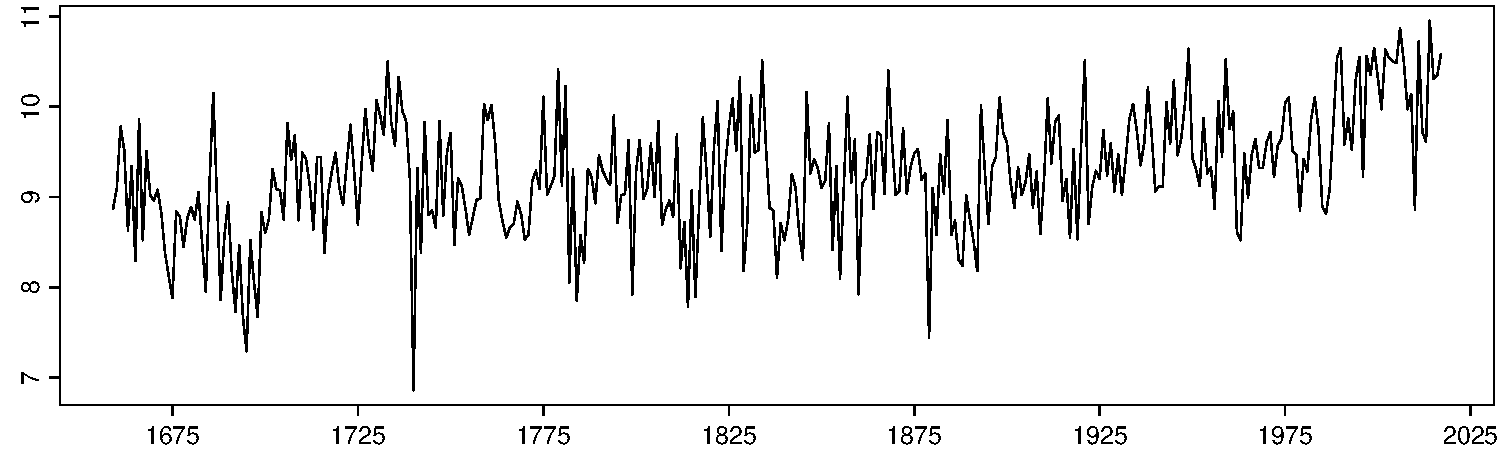
\includegraphics[width=0.9\textwidth]{Plots/temp_data.pdf}
\vspace{0.15cm}

\caption{Yearly mean temperature in Central England from 1659 to 2017 measured in $^\circ$C.}\label{temp_data}
\end{figure}


In this paper, we develop new methods to test for certain shape properties of a nonparametric time trend. We in particular construct a multiscale test which allows to identify local increases/decreases of the trend function. 
%We in particular construct a multiscale test for local increases/de\-creases of the trend function. The proposed test allows to identify, with a pre-specified statistical confidence, time regions where there is an increase/decrease in the trend. 
%identify subintervals on which the function $m$ deviates significantly from the null hypothesis of constancy. 
We develop our test in the context of the following model setting: We observe a time series $\{ Y_{t,T}: 1 \le t \le T \}$ of the form 
\begin{equation}\label{model-intro}
Y_{t,T} = m \Big( \frac{t}{T} \Big) + \varepsilon_t
\end{equation}
for $1 \le t \le T$, where $m: [0,1] \rightarrow \mathbb{R}$ is an unknown nonparametric regression function and the error terms $\varepsilon_t$ form a stationary time series process with $\ex[\varepsilon_t] = 0$. In a time series context, the design points $t/T$ represent the time points of observation and $m$ is a nonparametric time trend. As usual in nonparametric regression, we let the function $m$ depend on rescaled time $t/T$ rather than on real time $t$. A detailed description of model \eqref{model-intro} is provided in Section \ref{sec-model}.


Our multiscale test is developed step by step in Section \ref{sec-method}. Roughly speaking, the procedure can be outlined as follows: Let $H_0(u,h)$ be the hypothesis that $m$ is constant in the time window $[u-h,u+h] \subseteq [0,1]$, where $u$ is the midpoint and $2h$ the size of the window. In a first step, we set up a test statistic $\widehat{s}_T(u,h)$ for the hypothesis $H_0(u,h)$. In a second step, we aggregate the statistics $\widehat{s}_T(u,h)$ for a large number of different time windows $[u-h,u+h]$. We thereby construct a multiscale statistic which allows to test the hypothesis $H_0(u,h)$ simultaneously for many time windows $[u-h,u+h]$. In the technical part of the paper, we derive the theoretical properties of the resulting multiscale test. To do so, we come up with a proof strategy which combines strong approximation results for dependent processes with anti-concentration bounds for Gaussian random vectors. This strategy is of interest in itself and may be applied to other multiscale test problems for dependent data. As shown by our theoretical analysis, our multiscale test is a rigorous level-$\alpha$-test of the overall null hypothesis $H_0$ that $H_0(u,h)$ is simultaneously fulfilled for all time windows $[u-h,u+h]$ under consideration. Moreover, for a given significance level $\alpha \in (0,1)$, the test allows to make simultaneous confidence statements of the following form: We can claim, with statistical confidence $1-\alpha$, that there is an increase/decrease in the trend $m$ on all time windows $[u-h,u+h]$ for which the hypothesis $H_0(u,h)$ is rejected. Hence, the test allows to identify, with a pre-specified statistical confidence, time regions where the trend $m$ is increasing/decreasing. 


For independent data, multiscale tests have been developed in a variety of different contexts in recent years. In the regression context, \cite{ChaudhuriMarron1999,ChaudhuriMarron2000} introduced the so-called SiZer method which has been extended in various directions; see e.g.\ \cite{HannigMarron2006} where a refined distribution theory for SiZer is derived. \cite{HallHeckman2000} constructed a multiscale test on monotonicity of a regression function. \cite{DuembgenSpokoiny2001} developed a multiscale approach which works with additively corrected supremum statistics and derived theoretical results in the context of a continuous Gaussian white noise model. Rank-based multiscale tests for nonparametric regression were proposed in \cite{Duembgen2002} and \cite{Rohde2008}. More recently, \cite{ProkschWernerMunk2018} have constructed multiscale tests for inverse regression models. In the context of density estimation, multiscale tests have been investigated in \cite{DuembgenWalther2008}, \cite{RufibachWalther2010}, \cite{SchmidtHieber2013} and \cite{EckleBissantzDette2017} among others. 


Whereas a large number of multiscale tests for independent data have been developed in recent years, multiscale tests for dependent data are much rarer. Most notably, there are some extensions of the SiZer approach to a time series context. \cite{Rondonotti2004} and \cite{Rondonotti2007} have introduced SiZer methods for dependent data which can be used to find local increases/decreases of a trend and which may thus be regarded as an alternative to our multiscale test. However, these SiZer methods are mainly designed for data exploration rather than for rigorous statistical inference. Our multiscale method, in contrast, is a rigorous level-$\alpha$-test of the hypo\-thesis $H_0$ which allows to make simultaneous confidence statements about the time regions where the trend $m$ is increasing/decreasing. Some theoretical results for dependent SiZer methods have been derived in \cite{ParkHannigKang2009}, but only under a quite severe restriction: Only time windows $[u-h,u+h]$ with window sizes or scales $h$ are taken into account that remain bounded away from zero as the sample size $T$ grows. Scales $h$ that converge to zero as $T$ increases are excluded. This effectively means that only large time windows $[u-h,u+h]$ are taken into consideration. Our theory, in contrast, allows to simultaneously consider scales $h$ of fixed size and scales $h$ that converge to zero at various different rates. We are thus able to take into account time windows of many different sizes. \textcolor{red}{In Section \ref{subsec-method-comparison}, we compare our approach to SiZer methods in more detail.}


Our multiscale approach is also related to Wavelet-based methods: Similar to the latter, it takes into account different locations $u$ and resolution levels or scales $h$ simultaneously. However, while our multiscale approach is designed to test for local increases/decreases of a nonparametric trend, Wavelet methods are commonly used for other purposes. Among other things, they are employed for estimating/reconstructing nonparametric regression curves [see e.g.\ \cite{Donoho1995} or \cite{vonSachsMacGibbon2000}] and for change point detection [see e.g.\ \citet{ChoFryzlewicz2012}]. 


%Whereas a large number of multiscale tests for independent data have been developed in recent years, multiscale tests for dependent data are much rarer. Most notably, there are some extensions of the SiZer approach to a time series context. \cite{Rondonotti2004}, \cite{Rondonotti2007} and \cite{ParkHannigKang2009} have developed SiZer methods for dependent data which can be regarded as an alternative to our multiscale test. However, these SiZer methods are mainly designed for data exploration rather than rigorous statistical inference. Our multiscale method, in contrast, is a rigorous level-$\alpha$-test of the hypo\-thesis $H_0$, which is backed up by a complete asymptotic theory. Moreover, it allows to make simultaneous confidence statements about the time regions where the trend function $m$ is increasing/decreasing, which is not possible with the SiZer tools of \cite{Rondonotti2004}, \cite{Rondonotti2007} and \cite{ParkHannigKang2009}. Our multiscale approach is also related to Wavelet-based methods: It investigates the data on different intervals $[u-h,u+h]$. Similar to Wavelet-based procedures, it thus takes into account different locations $u$ and resolution levels $h$ simultaneously. Nevertheless, we are not aware of any Wavelet-based test for local increases/decreases of the nonparametric trend function in model \eqref{model-intro}. Wavelet methods have been used for other purposes in the literature such as estimating/reconstructing nonparametric regression functions [see e.g.\ \cite{Donoho1995} or \cite{vonSachsMacGibbon2000}] and change point detection [see e.g.\ \citet{ChoFryzlewicz2012}]. 


The test statistic of our multiscale method depends on the long-run error variance $\sigma^2 = \sum\nolimits_{\ell=-\infty}^{\infty} \cov(\varepsilon_0,\varepsilon_{\ell})$, which is usually unknown in practice. To carry out our multiscale test, we thus require an estimator of $\sigma^2$. Indeed, such an estimator is required for virtually all inferential procedures in the context of model \eqref{model-intro}. Hence, the problem of estimating $\sigma^2$ in model \eqref{model-intro} is of broader interest and has received a lot of attention in the literature; see \cite{MuellerStadtmueller1988}, \cite{Herrmann1992} and \cite{Hall2003} among many others. In Section \ref{sec-error-var}, 
%we discuss several estimators of $\sigma^2$ which are valid under different conditions on the error process $\{\varepsilon_t\}$. 
\textcolor{red}{we introduce a new difference-based estimator of $\sigma^2$ for the case that $\{ \varepsilon_t \}$ belongs to the class of AR($\infty$) processes}. This estimator improves on existing methods in several respects. 


The methodological and theoretical analysis of the paper is complemented by a simulation study in Section \ref{sec-sim} and an empirical application in Section \ref{sec-data}. In the simulation study, we examine the finite sample properties of our multiscale test and compare it to the dependent SiZer methods introduced in \cite{Rondonotti2004} and \cite{Rondonotti2007}. Moreover, we investigate the small sample performance of our estimator of $\sigma^2$ in the AR($p$) case and compare it to the estimator of \cite{Hall2003}. In Section \ref{sec-data}, we use our methods to analyse the temperature data from Figure \ref{temp_data} \textcolor{red}{as well as a sample of global temperature data}. 




%\setlength{\parindent}{10ex} 

\section{Introduction}\label{sec:intro}

Comparison of several regression curves is a classical topic in econometrics and statistics. In many cases of practical interest, the functional forms of the objective regression curves are unknown, hence, the parametric approach is not applicable. In this paper, we propose a novel approach that addresses this particular problem in a nonparametric context. Specifically, we present a new testing procedure for detecting differences between the nonparametric trends curves. 

In what follows, we consider a general panel framework with heterogeneous trends. Suppose we observe a panel of $n$ time series $\mathcal{W}_i = \{ (Y_{it},\mathbf{X}_{it}): 1 \le t \le T \}$ for\linebreak $1 \le i \le n$, where $Y_{it}$ are real-valued random variables and $\mathbf{X}_{it} = (X_{it,1},\ldots,X_{it,d})^\top$ are $d$-dimensional random vectors. Each time series $\mathcal{W}_i$ is modelled by the equation
\begin{equation}\label{eq:model}
Y_{it} = m_i \Big( \frac{t}{T} \Big) + \bfbeta_i^\top \mathbf{X}_{it} + \alpha_i + \varepsilon_{it}
\end{equation}
for $1 \le t \le T$, where $\bfbeta_i$ is a $d \times 1$ vector of unknown parameters, $\mathbf{X}_{it}$ is a $d\times 1$ vector of individual covariates or controls, $m_i$ is an unknown nonparametric (deterministic) trend function defined on $[0,1]$, $\alpha_i$ are so-called fixed effect error terms and \linebreak $\mathcal{E}_i = \{ \varepsilon_{it}: 1 \le t \le T \}$ is a zero-mean stationary error process. 


An important question in many applications is whether the observed time series have a common trend. In other words, the researchers would like to know if $m_i$ are the same for all $i$. Moreover, when there is evidence that this is not the case, one of the major related statistical problems is to determine which of the trends are different.% and whether we can group the time series with the similar trends together.
In addition, when two trends $m_i$ and $m_j$ are not the same, it may also be relevant to know in which time regions they differ from each other. In this paper, we introduce new statistical methods to approach these questions. In particular, we develop a test of the hypothesis that all time trends in model \eqref{eq:model} are the same. In this setting, the null hypothesis is formulated as 
\begin{align}\label{eq:null}
H_0: m_1 = m_2 = \ldots = m_n,
\end{align}
whereas the alternative hypothesis is 
$$H_1: \text{ there exists } x\in [0, 1] \text{ such that } m_i (x) \neq m_j(x) \text{ for some } 1\leq i < j \leq n.$$

The method that we propose does not only allow to test whether the null hypothesis is violated. It also allows to detect, with a given statistical confidence, which time trends are different and in which time regions they differ. More specifically, for any given interval $[u-h,u+h] \subseteq [0,1]$, consider the hypothesis
\[ H_0^{[i,j]}(u,h): m_i(w) = m_j(w) \text{ for all } w \in [u-h,u+h]. \] 
Here, we can regard $h$ as a bandwidth, a common tuning parameter in nonparametric estimation. The given interval $\interval_{(u, h)} = [u-h,u+h] \subseteq [0,1]$ is then fully characterized by $u$, its center (a location parameter), and $h$, the bandwidth. In order to determine the regions where the time trends are different, we consider a broad range of pairs $(u, h)$ with the property that they fully cover the unit interval $[0, 1]$. Formally, let \linebreak $\grid := \{(u, h): \interval_{(u, h)} = [u-h, u+h] \subseteq [0,1]\}$ be a grid of location-bandwidth points such that 
\begin{align*}
\bigcup_{(u, h) \in \grid}  \interval_{(u, h)} = [0,1].
\end{align*}
We then reformulate our null hypothesis \eqref{eq:null} as
\begin{align*}
H_0: \ & \text{The hypotheses } H_0^{[i,j]}(u,h) \text{ hold true for all intervals }  \interval_{(u, h)}, (u, h) \in \grid, \\ & \text{ and for all } 1 \le i < j \le n. 
\end{align*} 
$H_0^{[i,j]}(u,h)$ can thus be viewed as a local null hypothesis that characterizes the behavior of two trend functions only locally, whereas $H_0$ specified in \eqref{eq:null} is the global null hypothesis that is concerned with the comparison of all of the trends on the whole unit interval.

In this paper, we introduce a method that allows us to test the hypotheses $H_0^{[i,j]}(u,h)$  simultaneously for all pairs $(i, j)$ and for all intervals $\interval_{(u, h)}$ under consideration. Specifically, we develop a multiscale test for the model \eqref{eq:model}. The underlying idea of any multiscale test is to consider a number of test statistics (each corresponding to a different set of values of some tuning parameters) all at once rather than to perform a separate test for each single test statistics. In our case, this means testing many local null hypotheses $H_0^{[i,j]}(u,h)$ simultaneously which leads to a well-known multiple testing problem. Our method accounts for this problem by using appropriate critical values that depend on the scale of the problem, i.e. on the number of hypotheses tested simultaneously and the relationship between them. In the paper, we show that the suggested procedure for obtaining critical values leads to good theoretical properties of the proposed test: it has the correct (asymptotic) level and an (asymptotic) power of one against a certain class of local alternatives. %Moreover, we prove that when testing at a given level $\alpha$, the probability of rejecting even one local null hypothesis is no more than this level $\alpha$.

Trend comparison is a common statistical problem that arises in various contexts. For example, in economics the researchers compare trends in real gross domestic product across several countries \citep[][]{Grier1989}, in yield over time of US Treasury bills at different maturities \citep[][]{Park2009}, or the evolution of long-term interest rates in a number of countries \citep[][]{Christiansen1997}. In finance, comparison and subsequent classification of the trends of market fragmentation can be used to assess the market quality in the European stock market (\citeauthor{VogtLinton2017}, \citeyear{VogtLinton2017}, \citeyear{VogtLinton2020}). In climatology, the temperature time series in different geographical areas are investigated in the context of the regional and global warming trends \citep[][]{KarolyWu2005}. Finally, in industry, mobile phone providers are interested in finding the differences between the cell phone download activity in various locations \citep[][]{DegrasWu2012}.


In the statistical literature, the problem of testing whether the observed time series all have the same trend  has been widely studied, and tests for equality of trends or regression curves have been developed in \cite{HaerdleMarron1990}, \cite{Hall1990}, \linebreak \cite{Delgado1993} and \cite{DegrasWu2012} among many others. Versions of model \eqref{eq:model} with a parametric trend are considered in \cite{Vogelsang2005}, \cite{Sun2011} and \cite{Xu2012} among others. In the nonparametric context, \cite{LiChenGao2010}, \cite{Atak2011}, \cite{Robinson2012} and \cite{ChenGaoLi2012} studied panel models under the assumption that the observed time series have a common time trend. However, in many applications the restriction of including a common time trend in the model is questionable at best. For instance, when we observe a large number of time series it is reasonable to expect that at least some of the trends are different from the others. Consequently, it often makes sense to relax the assumption of a common trend, which leads to more flexible panel settings with heterogeneous trends. Such models have been studied, for example, in \cite{DegrasWu2012},  \cite{Zhang2012} and \cite{Hidalgo2014}. \cite{DegrasWu2012} consider the problem of testing $H_0$ in a model that is a special case of \eqref{eq:model} and does not include additional regressors. \cite{ChenWu2018} develop theory for a very similar model framework but under more general conditions on the error terms. \linebreak \cite{Zhang2012} investigate the problem of testing the hypothesis $H_0$ in a slightly restricted version of model \eqref{eq:model}, where $\bfbeta_i = \bfbeta$ for all $i$. All of these tests have an important drawback: they involve classical nonparametric estimation of the trend functions that depends on one or several bandwidth parameters, which imposes a certain limit on the applicability of such tests since in most cases it is far from clear how to choose bandwidth parameters in an appropriate way. Contrary to the aforementioned methods, our multiscale testing procedure allows us to consider a large collection of bandwidths simultaneously avoiding the problem of choosing only one bandwidth altogether.

Recently, \cite{KhismatullinaVogt2021} proposed a new inference method that allows researchers to detect differences between epidemic time trends in the context of the COVID-19 pandemic. In their paper, the authors present a statistically rigorous procedure that, similarly to ours, not only allows to compare trends across different countries, but to pinpoint the time intervals where the differences occur as well. Moreover, they also circumvent the need to pick a bandwidth parameter by using a multiscale testing approach. However, the model in \cite{KhismatullinaVogt2021} is only a special case of the model \eqref{eq:model} which includes neither the covariates $\mathbf{X}_{it}$, nor the fixed effects $\alpha_i$. Furthermore, the authors place major restriction on the error terms: in their model, $\varepsilon_{it}$ are independent across $t$. In contrast, our model \eqref{eq:model} can be regarded as a generalized version of theirs that allows for a wider range of economic and financial applications.

%This is a general problem concerning essentially all tests based on nonparametric curve estimators. There are of course many theoretical results on optimal bandwidth choice for estimation purposes. However, the optimal bandwidth for curve estimation is usually not optimal for testing. Optimal bandwidth choice for tests is indeed an open problem, and only little theory for simple cases is available \citep[][]{GaoGijbels2008}. Since tests based on nonparametric curve estimators are commonly quite sensitive to the choice of bandwidth and theory for optimal bandwidth selection is not available, it appears preferable to work with bandwidth-free tests. A classical way to obtain a bandwidth-free test of the hypothesis $H_0$ is to use CUSUM-type statistics which are based on partial sum processes. This approach is taken in \cite{Hidalgo2014}. A more modern approach to obtain a bandwidth-free test is to employ multiscale methods.

%More specifically, the basic idea is as follows: Let $S_h$ be a test statistic for the null hypothesis of interest, which depends on the bandwidth $h$. Rather than considering only a single statistic $S_h$ for a specific bandwidth $h$, a multiscale approach simultaneously considers a whole family of statistics $\{S_h: h \in \mathcal{H} \}$, where $\mathcal{H}$ is a set of bandwidth values. The multiscale test then proceeds as follows: For each bandwidth or scale $h$, one checks whether $S_h > q_h(\alpha)$, where $q_h(\alpha)$ is a bandwidth-dependent critical value (for given significance level $\alpha$). The multiscale test rejects if $S_h > q_h(\alpha)$ for at least one scale $h$. The main theoretical difficulty in this approach is of course to derive appropriate critical values $q_h(\alpha)$. Specifically, the critical values $q_h(\alpha)$ need to be determined such that the multiscale test has the correct (asymptotic) level, that is, such that $\pr (S_h > q_h(\alpha) \text{ for some } h \in \mathcal{H} ) = (1-\alpha) + o(1)$. 


%Multiscale methods have been developed for a variety of different test problems in recent years. \cite{ChaudhuriMarron1999, ChaudhuriMarron2000} introduced the so-called SiZer method which has been extended in various directions; see for example \cite{HannigMarron2006} and \cite{Rondonotti2007}. \cite{HorowitzSpokoiny2001} proposed a multiscale test for the parametric form of a regression function. \cite{DuembgenSpokoiny2001} constructed a multiscale approach which works with additively corrected supremum statistics. This general approach has been very influential in recent years and has been further developed in numerous ways; see for example \cite{Duembgen2002}, \cite{Rohde2008} and \cite{ProkschWernerMunk2018} for multiscale methods in the regression context and \cite{DuembgenWalther2008}, \cite{RufibachWalther2010}, \cite{SchmidtHieber2013} and \cite{EckleBissantzDette2017} for methods in the context of density estimation. Importantly, all of these studies are restricted to the case of independent data. It turns out that it is highly non-trivial to extend the multiscale approach of \cite{DuembgenSpokoiny2001} to the case of dependent data. A first step into this direction has recently been made in \cite{KhismatullinaVogt2020}. They developed multiscale methods to test for local increases/decreases of the nonparametric trend function $m$ in the univariate time series model $Y_t = m(t/T) + \varepsilon_t$.  


To sum up, the main theoretical contribution of the current paper is the multiscale testing method that allows to make simultaneous confidence statements about which of the time trends are distinct and the regions where they differ. We believe that currently there are no equivalent statistical methods. Even though tests for equality of the trends have been developed already for a while, most existing procedures allow only to test whether the trend curves are all the same or not, but they almost never allow to infer which curves are different and where. To the best of our knowledge, the only two exceptions are \cite{KhismatullinaVogt2021}, whose contribution is briefly discussed above, and \cite{Park2009} who developed SiZer methods for the comparison of nonparametric trend curves in a significantly simplified version of the model \eqref{eq:model}. In addition to restricted model, \cite{Park2009} derive theoretical results for their analysis only for the special case of observing only two time series, whereas in other cases, the algorithm is provided without detailed proof.

The structure of the paper is as follows. Section \ref{sec:model} introduces the model setting and the necessary technical assumptions that are required for the theory. The multiscale test is developed step by step in Section \ref{sec:test}. The main theoretical results are presented in Section \ref{sec:theo}. Section \ref{sec:para} deals with estimating the unknown parameters necessary for construction of the test statistics. To keep the discussion as clear as possible, we include in the main text of the paper only the essential parts of the theoretical arguments, and the technical details and extended proofs are deferred to the Appendix. Section \ref{sec:conclusion} concludes.


\section{The model}\label{sec:model}

Throughout the paper, we adopt the following notation. For a real-valued vector \linebreak $\mathbf{v} = (v_1, \ldots, v_m)\in\reals^m$, we write $|\mathbf{v}| = \big(\sum_{i=1}^m v_i^2\big)^{1/2}$ and $|\mathbf{v}|_q = \big(\sum_{i=1}^m v_i^q\big)^{1/q}$ respectively. For a random vector $\mathbf{V}$, we define it's $\mathcal{L}^q, q>1$ norm as $||\mathbf{V}||_q = \big(\ex |\mathbf{V}|^q\big)^{1/q}$. For the particular case $q = 2$, we write $||\mathbf{V}|| := ||\mathbf{V}||_2$.

\textcolor{black}{Let $\epsilon_t, t \in \integers,$ be independent and identically distributed (i.i.d.) random variables and let $\mathbf{L}$ be a measurable real-valued vector function such that $\mathbf{L}(\ldots, \epsilon_{t-1}, \epsilon_t)$ is a properly defined random variable. Denote $\mathcal{F}_t  = (\ldots, \epsilon_{t-1}, \epsilon_t)$.}  Following \cite{Wu2005}, we define the \textit{physical dependence measure} for the process $\mathbf{L}(\mathcal{F}_t)$ as the following:
\begin{align}\label{eq:physical_dep}
 \delta_q(\mathbf{L}, t) = || \mathbf{L}(\mathcal{F}_t) - \mathbf{L}(\mathcal{F}_t^\prime) ||_q,
\end{align}
where $\mathcal{F}_t^\prime  = (\ldots, \epsilon_{-1}, \epsilon^\prime_0, \epsilon_1, \ldots, \epsilon_{t-1}, \epsilon_t)$ is a coupled process of $\mathcal{F}_t$ with $\epsilon_0^\prime$ being an i.i.d. copy of $\epsilon_0$. Intuitively, $\delta_q(\mathbf{L}, t)$ measures the dependency of $\mathbf{L}(\mathcal{F}_t)$ on $\epsilon_0$, i.e., how replacing $\epsilon_0$ by an i.i.d. copy while keeping all other innovations in place affects the output $\mathbf{L}(\mathcal{F}_t)$.

\subsection{Setting}\label{subsec:model_setting}

As was already briefly discussed in Section \ref{sec:intro}, the model setting is as follows. We observe a panel of $n$ time series $\mathcal{W}_i = \{(Y_{it}, \mathbf{X}_{it}): 1 \le t \le T \}$ of length $T$ for $1 \le i \le n$. Each time series $\mathcal{W}_i$ satisfies the model equation 
\begin{equation}\label{eq:model_full}
Y_{it} = \bfbeta^\top_i \mathbf{X}_{it} + m_i \Big( \frac{t}{T} \Big) + \alpha_i + \varepsilon_{it} 
\end{equation}
for $1 \le t \le T$, where $\bfbeta_i$ is a $d \times 1$ vector of unknown parameters, $\mathbf{X}_{it}$ is a $d\times 1$ vector of individual covariates, $m_i$ is an unknown nonparametric trend function defined on $[0,1]$ with $\int_0^1 m_i(u) du = 0$ for all $i$, $\alpha_i$ is a (deterministic or random) intercept term and \linebreak $\mathcal{E}_i = \{ \varepsilon_{it}: 1 \le t \le T \}$ is a zero-mean stationary error process. As common in nonparametric regression, the trend functions $m_i$ in model \eqref{eq:model_full} depend on rescaled time $t/T$ rather than on real time $t$. Using rescaled time is equivalent to restricting the domain of the functions to the unit interval which in turn allows us to apply the usual asymptotic arguments. Discussion about the application of the rescaled time in the context of nonparametric estimation can be found in \ \cite{Robinson1989}, \cite{Dahlhaus1997} and \cite{VogtLinton2014}. The condition $\int_0^1 m_i(u) du = 0$ for all $i$ is a necessary identification condition due the presence of  $\alpha_i$. Without imposing this condition, we can freely increase the functions $m_i$ by any (positive or negative) constant $c_i$ while simultaneously subtract the same constant from the intercept term $\alpha_i$:
$$Y_{it} = [m_i(t/T) + c_i] + \bfbeta_i^\top \mathbf{X}_{it} + [\alpha_i - c_i] + \varepsilon_{it}.$$
The term $\alpha_i$ can be regarded as an additional error component. In the econometrics literature, it is commonly called a fixed effect and is often interpreted as the term which captures unobserved characteristics of the time series $\mathcal{W}_i$ that remain constant over time. We allow the error terms $\alpha_i$ to be dependent across $i$ in an arbitrary way. Hence, by including them in model equation \eqref{eq:model_full}, we allow the $n$ time series $\mathcal{W}_i$ in our panel to be correlated with each other. Whereas the terms $\alpha_i$ may be correlated, the error processes $\mathcal{E}_i$ are assumed to be independent across $i$. As usual in nonparametric estimation, we also assume that all the trend functions $m_i(\cdot)$ are continuously differentiable on $[0, 1]$. Technical conditions regarding the model are discussed further in this section.

Finally, throughout the paper we restrict attention to the case where the number of time series $n$ in model \eqref{eq:model_full} is fixed. Extending our theoretical results to the case where $n$ slowly grows with the sample size $T$ is a possible topic for further research.

\subsection{Assumptions}\label{subsec:model_assumptions}

Each process $\mathcal{E}_i$ is supposed to satisfy the following conditions: 

\begin{enumerate}[label=(C\arabic*),leftmargin=1.05cm]

\item \label{C-err1} \textcolor{black}{The variables $\varepsilon_{it}$ are independent across $i$} and for each $i$ the variables $\varepsilon_{it}$ allow for the representation $\varepsilon_{it} = G_i(\ldots,\eta_{it-1},\eta_{it})$, where $\eta_{it}$ are i.i.d.\ random variables across $t$ and $G_i: \reals^\integers \rightarrow \reals$ is a measurable function. Denote \linebreak $\mathcal{J}_{it} = (\ldots,\eta_{it-2},\eta_{it-1},\eta_{it})$.

\item \label{C-err2} For all $i$ it holds that $\ex[\varepsilon_{it}] =0$ and $\| \varepsilon_{it} \|_q < \infty$ for some $q > 4$.
\end{enumerate}
Assumption \ref{C-err1} can be translated as the restriction on the error process $\mathcal{E}_i$ to be stationary and causal (in the sense that $\varepsilon_{it}$ does not depend on the future innovations $\eta_{is},\, s >t$). The class of error processes that satisfies the condition \ref{C-err1} is massive, and includes linear processes, their nonlinear transformation, as well as a large variety of nonlinear processes such as Markov chain models and nonlinear autoregressive models \citep[][]{Wu2016}. Assumption \ref{C-err2} is a standard moment condition.

Following \cite{Wu2005}, we impose conditions on the dependence structure of the error processes $\mathcal{E}_i$ in terms of the physical dependence measure $\delta_q(G_i, t)$ defined in \eqref{eq:physical_dep}. In particular, we assume the following: 
\begin{enumerate}[label=(C\arabic*),leftmargin=1.05cm]
\setcounter{enumi}{2}

\item \label{C-err3} Define $\Theta_{i, t,q} = \sum\nolimits_{s \ge t} \delta_q(G_i, s)$ for $t \ge 0$. For each $i$ it holds that \linebreak
$\Theta_{i, t,q} = O ( t^{-\tau_q} (\log t)^{-A} )$,  
where $A > \frac{2}{3} (1/q + 1 + \tau_q)$ and \linebreak $\tau_q = \{q^2 - 4 + (q-2) \sqrt{q^2 + 20q + 4}\} / 8q$. 

\end{enumerate}

For fixed $i$ and $t$, $\Theta_{i, t,q}$ measures the cumulative effect of $\eta_0$ on $(\varepsilon_{is})_{s\geq t}$ in terms of $\mathcal{L}^q$-norm. Condition \ref{C-err3} assumes that the overall cumulative effect is finite and puts some restrictions on the rate of decay of $\Theta_{i, t,q}$. Assumption \ref{C-err3} is fulfilled by a wide range of stationary processes $\mathcal{E}_i$. For a detailed discussion of assumption \ref{C-err3}, as well as assumptions \ref{C-err1}--\ref{C-err2} and some examples of the error processes that satisfy these conditions, see \cite{KhismatullinaVogt2020}.

Regarding the independent variables $ \mathbf{X}_{it}$, we assume the following for each $i$:

\begin{enumerate}[label=(C\arabic*),leftmargin=1.05cm]
\setcounter{enumi}{3}

\item \label{C-reg1} The covariates $ \mathbf{X}_{it}$ allow for the representation $ \mathbf{X}_{it} = \mathbf{H}_i(\ldots,u_{it-1},u_{it})$ with $u_{it}$ being i.i.d.\  across $t$ random variables and $\mathbf{H}_i := (H_{i1}, H_{i2}, \ldots, H_{id})^\top: \reals^\integers \rightarrow \reals^d$ being a measurable function such that $\mathbf{H}_i(\mathcal{U}_{it})$ is well defined. We denote $\mathcal{U}_{it} = (\ldots, u_{it-1}, u_{it})$.

\item \label{C-reg2} Let $\mathbf{N}_i$ be the $d\times d$ matrix with $kl$-th entry $n_{i, kl}= \ex[H_{ik}(\mathcal{U}_{i0})H_{il}(\mathcal{U}_{i0})]$. We assume that the smallest eigenvalue of $\mathbf{N}_i$ is strictly bigger than $0$.

\item \label{C-reg3} Let $\ex [\mathbf{H}_{i}(\mathcal{U}_{i0})]=\mathbf{0}$ and $||\mathbf{H}_{i}(\mathcal{U}_{it})||_{q^\prime} <\infty$ for some $q^\prime > \max\{ 2\theta, 4\}$, where $\theta$ will be introduced further in Assumption \ref{C-grid}.
\item \label{C-reg4} $\sum_{s=0}^\infty \delta_{q^\prime}(\mathbf{H}_i, s)<\infty$ for $q^\prime$ from Assumption \ref{C-reg3}.
\item \label{C-reg5} For each $i$ it holds that $\sum_{s=t}^{\infty} \delta_{q^\prime}(\mathbf{H}_{i}, s)= O(t^{-\alpha}) $ for $q^\prime$ from Assumption \ref{C-reg3} and for some $\alpha > 1/2 - 1/{q^\prime}$.
\end{enumerate}

As with the error processes $\mathcal{E}_i$, $\mathbf{X}_i$ is guaranteed to be stationary and causal by Assumption \ref{C-reg1}. Assumptions \ref{C-reg2} and \ref{C-reg3} are technical conditions that prevent asymptotic multicollinearity and ensure that all the necessary moments exist, respectively. Moreover, similarly to the restriction on the error processes, we also employ the definition of the physical dependence measure $ \delta_{q}(\cdot, \cdot)$ in Assumptions \ref{C-reg4} - \ref{C-reg5}, thus, making certain that the cumulative effect of the innovation $u_0$ on $(\mathbf{X}_{it})_{t\geq 0}$ is finite. 



To be able to prove the main theorems in Section \ref{sec:test}, we need additional assumptions on the relationship between the covariates and the error process.

\begin{enumerate}[label=(C\arabic*),leftmargin=1.05cm]
\setcounter{enumi}{8}
\item \label{C-reg-err1} $\mathbf{X}_{it}$ (elementwise) and $\varepsilon_{is}$ are uncorrelated for each $t, s\in \{1, \ldots, T\}$.
\item \label{C-reg-err2} Let $\zeta_{i, t} = (u_{it}, \eta_{it})^\top$. Define $\mathcal{I}_{it} = (\ldots, \zeta_{i, t-1}, \zeta_{i, t})$ and $\mathbf{U}_i(\mathcal{I}_{it}) =  \mathbf{H}_i(\mathcal{U}_{it})G_i(\mathcal{J}_{it})$. With this notation at hand, we assume that $\sum_{s=0}^\infty \delta_2(\mathbf{U}_i, s)<\infty$.

\end{enumerate}
Assumption \ref{C-reg-err1} is a slightly relaxed independence assumption: even though we do not require the covariates $\mathbf{X}_{it}$ to be completely independent with the error terms $\varepsilon_{it}$, our theoretical results depend upon them being uncorrelated. We in particular need this restriction in order to prove asymptotic consistency for the differencing estimator $\widehat{\bfbeta}_i$ of $\bfbeta_i$ proposed in Section \ref{subsec:para:beta}. In principle, it would be possible to relax this assumption even further, but that would involve much more complicated estimation procedure of $\bfbeta_i$ and more arduous technical arguments. Assumption \ref{C-reg-err2} ensures short-range dependence among the variables in our model. Again, we can interpret this as the fact that the cumulative effect of a single error on all future values is bounded.

We employ these assumptions to prove the main theoretical results in our paper. For detailed proofs, we refer the reader to the Appendix.

\begin{remark}
The conditions \ref{C-reg1}--\ref{C-reg-err2} can be relaxed to cover nonstationary regressors as well as stationary ones. For example, \ref{C-reg1} may then be replaced by
\begin{enumerate}[label=(C\arabic*$^\ast$),leftmargin=1.05cm]
\setcounter{enumi}{3}
\item \label{C-reg1-star} The covariates $ \mathbf{X}_{it}$ allow for the representation $ \mathbf{X}_{it} = \mathbf{H}_i(t; \ldots,u_{it-1},u_{it})$ with $u_{it}$ being i.i.d.\ random variables and $\mathbf{H}_i := (H_{i1}, H_{i2}, \ldots, H_{id})^\top: \reals^\integers \rightarrow \reals^d$ is a measurable function such that $\mathbf{H}_i(t;\mathcal{U}_{it})$ is well defined. 
\end{enumerate} 
The other assumptions can be adjusted accordingly. Our main theoretical results will in principle still hold in this case, however, the complexity of the technical arguments will increase drastically. Hence, for the sake of clarity, we restrict our attention only to stationary  covariates $\mathbf{X}_{it}$. 
\end{remark}


\section{Testing procedure}\label{sec:test}

In this section, we develop a multiscale testing procedure for the problem of comparison of the trend curves $m_i$ in model \eqref{eq:model_full}.  As we will see, the proposed multiscale method does not only allow to test whether the null hypothesis is violated. It also provides information on where violations occur. More specifically, it allows to identify, with a pre-specified confidence, (i) trend functions which are different from each other and (ii) time intervals where these trend functions differ.

\subsection{Preliminary steps}\label{subsec:test:prep}

Testing the null hypothesis $H_0: m_1 = m_2 = \ldots = m_n$ in model \eqref{eq:model_full} is a challenging task not only because it involves nonparametric estimation of the functions $m_i(\cdot)$, but also due to the presence of an unknown fixed term $\alpha_i$ and a vector of unknown parameters $\bfbeta_i$. It is clear that if $\alpha_i$ and $\bfbeta_i$ are known, the problem of testing for the common time trend would be greatly simplified. That is, we would test $H_0: m_1 = m_2 = \ldots = m_n$ in the model
\begin{align*}
Y_{it} - \alpha_i - \bfbeta_i^\top \mathbf{X}_{it} & =: Y_{it}^\circ\\
					& = m_i \Big( \frac{t}{T} \Big) + \varepsilon_{it}, 
\end{align*}
which is a standard nonparametric regression equation. However, in reality the variables $Y_{it}^\circ$ are not observed since the intercept $\alpha_i$ and the coefficients $\bfbeta_i$ are not known. Nevertheless, given appropriate estimators $\widehat{\alpha}_i$ and $\widehat{\bfbeta}_i$, we can consider
\begin{align*}
	\widehat{Y}_{it} := Y_{it} -\widehat{\alpha}_i - \widehat{\bfbeta}_i^\top \mathbf{X}_{it} =(\bfbeta_i - \widehat{\bfbeta}_i)^\top \mathbf{X}_{it} + m_i \Big( \frac{t}{T} \Big) + \big( \alpha_i - \widehat{\alpha}_i \big) + \varepsilon_{it}. 
\end{align*}
Thus, the unobserved variables $Y_{it}^\circ$ can be approximated by $\widehat{Y}_{it}$, and in what follows we show that under some mild conditions on $\widehat{\alpha}_i$ and $\widehat{\bfbeta}_i$, this approximation is indeed sufficient for our analysis. 

But before we proceed further, we show how to construct consistent estimates $\widehat{\alpha}_i$ and $\widehat{\bfbeta}_i$. To begin with, we focus on the estimation of the vector of unknown parameters $\bfbeta_i$. We construct the estimator  $\widehat{\bfbeta}_i$ in the following way.

For each $i$, we consider the time series $\{\Delta Y_{it}: 2 \leq t \leq T\}$ of the differences \linebreak $\Delta Y_{it} = Y_{it} - Y_{i t-1}$. We can write
\begin{align*}
	\Delta Y_{it} = Y_{it} - Y_{i t-1} =\bfbeta_i^\top \Delta \mathbf{X}_{it} + \bigg(m_i \Big( \frac{t}{T} \Big) - m_i \Big(\frac{t-1}{T}\Big)\bigg) + \Delta \varepsilon_{it},
\end{align*}
where $\Delta  \mathbf{X}_{it} =  \mathbf{X}_{it} -  \mathbf{X}_{it-1}$ and $ \Delta \varepsilon_{it} = \varepsilon_{it} - \varepsilon_{i t-1}$. Since $m_i(\cdot)$ is Lipschitz (by our assumption that $m_i(\cdot)$ is continuously differentiable on $[0, 1]$), we can use the fact that $ \big|m_i \big( \frac{t}{T} \big) - m_i \big(\frac{t-1}{T}\big) \big| = O\big(\frac{1}{T}\big)$ and rewrite 
\begin{align}\label{model_with_regs}
	\Delta Y_{it} = \bfbeta_i^\top \Delta \mathbf{X}_{it} + \Delta \varepsilon_{it} + O\Big(\frac{1}{T}\Big).
\end{align}

Now, for each $i$ we employ the least squares estimation method to estimate $\bfbeta_i$ in \eqref{model_with_regs}, treating $\Delta \mathbf{X}_{it}$ as the regressors and $\Delta Y_{it}$ as the response variable. That is, we propose the following differencing estimator:
\begin{align}\label{eq:beta:est}
\widehat{\bfbeta}_i = \Big( \sum_{t=2}^T \Delta \mathbf{X}_{it} \Delta \mathbf{X}_{it}^\top \Big)^{-1} \sum_{t=2}^T \Delta \mathbf{X}_{it} \Delta Y_{it}
\end{align}
We will show in Section \ref{subsec:para:beta} that $\widehat{\bfbeta}_i$ is a consistent estimator of $\bfbeta_i$ with the property $\bfbeta_i - \widehat{\bfbeta}_i = O_P(T^{-1/2})$.

Next, given $\widehat{\bfbeta}_i$, consider an appropriate estimator $\widehat{\alpha}_{i}$ for the intercept $\alpha_i$ calculated by
\begin{align}\label{alpha-est}
\widehat{\alpha}_i &= \frac{1}{T}\sum_{t=1}^T \big(Y_{it} - \widehat{\bfbeta}_i^\top \mathbf{X}_{it}\big) = \frac{1}{T}\sum_{t=1}^T \big(\bfbeta_i^\top \mathbf{X}_{it} - \widehat{\bfbeta}_i^\top \mathbf{X}_{it} + \alpha_i + m_i(t/T) + \varepsilon_{it}\big) =\\
&= \big(\bfbeta_i - \widehat{\bfbeta}_i \big)^\top\frac{1}{T}\sum_{t=1}^T  \mathbf{X}_{it} + \alpha_i + \frac{1}{T}\sum_{i=1}^T m_i(t/T) + \frac{1}{T}\sum_{i=1}^T \varepsilon_{it}.\nonumber
\end{align}
Note that $\frac{1}{T}\sum_{i=1}^T \varepsilon_{it} = O_P(T^{-1/2})$ and $\frac{1}{T}\sum_{i=1}^T m_i(t/T) = O(T^{-1})$ due to Lipschitz continuity of $m_i$ and normalization $\int_{0}^1 m_i(u)du = 0$. Furthermore, $\frac{1}{T}\sum_{t=1}^T  \mathbf{X}_{it} = O_P(1)$ by Chebyshev's inequality and $\widehat{\bfbeta}_i - \bfbeta_i = O_P (T^{-1/2})$. Plugging all these results together in \eqref{alpha-est}, we get that $\widehat{\alpha}_i - \alpha_i = O_P(T^{-1/2})$. Thus, the unobserved variables \linebreak $Y_{it}^\circ := Y_{it} - \bfbeta_i^\top \mathbf{X}_{it} - \alpha_i = m_i(t/T) + \varepsilon_{it}$ can be well approximated by $\widehat{Y}_{it} $ since \linebreak $\widehat{Y}_{it} = Y_{it} -\widehat{\alpha}_i - \widehat{\bfbeta}_i^\top \mathbf{X}_{it} = Y_{it}^\circ + O_P(T^{-1/2})$.

We now turn to the estimator of the long-run error variance $\sigma_i^2 = \sum\nolimits_{\ell=-\infty}^{\infty} \cov(\varepsilon_{i0}, \varepsilon_{i\ell})$ which is necessary for the construction of the test statistics later on. For the moment, we assume that the long-run variance does not depend on $i$, that is $\sigma_i^2 = \sigma^2$ for all $i$. We will need this further for conducting the testing procedure properly. Nevertheless, we keep the indices throughout the paper in order to be congruous in notation. We further let $\widehat{\sigma}_i^2$ be an estimator of $\sigma_i^2$ which is computed from the constructed sample $\{ \widehat{Y}_{it}: 1 \le t \le T \}$. We thus regard $\widehat{\sigma}_i^2 = \widehat{\sigma}_i^2(\widehat{Y}_{i1},\ldots,\widehat{Y}_{iT})$ as a function of the variables $\widehat{Y}_{it}$ for $1 \le t \le T$. Hence, whereas the true long-run variance is the same for all time series, the estimators are different. Throughout the section, we assume that $\widehat{\sigma}_i^2 = \sigma_i^2 + o_p(\rho_T)$ where the conditions on $\rho_T$ will be provided further in Section \ref{sec:theo}. Details on how to construct $\widehat{\sigma}_i^2$ are deferred to Section \ref{subsec:para:lrv}. 

\subsection{Construction of the test statistics}\label{subsec:test:stat}

We are now ready to introduce the multiscale statistic for testing the hypothesis \linebreak $H_0: m_1 = m_2 = \ldots = m_n$. For any pair of time series $i$ and $j$ and for any location-bandwidth pair $(u, h)$, we define the kernel averages
\begin{align}\label{eq:psi_hat_ij}
 \widehat{\psi}_{ij,T}(u,h) = \sum\limits_{t=1}^T w_{t,T}(u,h)(\widehat{Y}_{it} - \widehat{Y}_{jt}),
 \end{align}
where $w_{t,T}(u,h)$ are the local linear kernel weights calculated by the following formula:
\begin{equation}\label{eq:weights}
w_{t,T}(u,h) = \frac{\Lambda_{t,T}(u,h)}{ \{\sum\nolimits_{t=1}^T \Lambda_{t,T}(u,h)^2 \}^{1/2} }, 
\end{equation}
where
\[ \Lambda_{t,T}(u,h) = K\Big(\frac{\frac{t}{T}-u}{h}\Big) \Big[ S_{T,2}(u,h) - \Big(\frac{\frac{t}{T}-u}{h}\Big) S_{T,1}(u,h) \Big], \]
$S_{T,\ell}(u,h) = (Th)^{-1} \sum\nolimits_{t=1}^T K(\frac{\frac{t}{T}-u}{h}) (\frac{\frac{t}{T}-u}{h})^\ell$ for $\ell = 1,2$ and $K$ is a kernel function. As common in the nonparametric estimation, we assume that $K$ has the following properties: 
\begin{enumerate}[label=(C\arabic*),leftmargin=1.05cm]
\setcounter{enumi}{10}
\item \label{C-ker} The kernel $K$ is non-negative, symmetric about zero and integrates to one. Moreover, it has compact support $[-1,1]$ and is Lipschitz continuous, that is,\linebreak $|K(v) - K(w)| \le C |v-w|$ for any $v,w \in \reals$ and some constant $C > 0$. 
\end{enumerate} 
Assumption \ref{C-ker} allows us to use the usual kernel functions such as rectangular, Epanechnikov and Gaussian kernels.

We regard the kernel average $\widehat{\psi}_{ij,T}(u,h)$ as a measure of the distance between the two trend curves $m_i$ and $m_j$ on the interval $\interval_{(u, h)} = [u-h,u+h]$. However, instead of working directly with the kernel averages $\widehat{\psi}_{ij,T}(u,h)$, we replace them by their normalized and corrected version:
\begin{align}\label{eq:psi_zero_ij}
\hat{\psi}^0_{ij,T}(u, h) =  \Big|\frac{\widehat{\psi}_{ij,T}(u,h)}{(\widehat{\sigma}_i^2 + \widehat{\sigma}_j^2)^{1/2}}\Big| - \lambda(h).
\end{align}
Here, $\lambda(h) = \sqrt{2 \log \{ 1/(2h) \}}$ is an additive correction term that balances the significance of many test statistics that correspond to different values of bandwidth parameters (see the discussion on this topic and comparison between multiscale testing procedures with and without this correction term in \citet{KhismatullinaVogt2020}).

We now aggregate the test statistics $\hat{\psi}^0_{ij, T}(u,h)$ for all $i$ and $j$ and a wide range of different locations $u$ and bandwidths (scales) $h$:
\begin{align}\label{eq:Psi_hat}
	\widehat{\Psi}_{n,T} = \max_{1 \le i < j \le n}\max_{(u,h) \in \mathcal{G}_T} \hat{\psi}^0_{ij,T}(u, h),
\end{align}

In \eqref{eq:Psi_hat}, $\mathcal{G}_T$ stands for the set of location-bandwidth pairs $(u, h)$ that was mentioned in Section \ref{sec:intro}. We use the subscript $T$ in $\grid_T$ to point out that the choice of the grid depends on the sample size $T$. Specifically, throughout the paper, we suppose that $\mathcal{G}_T$ is some subset of $\mathcal{G}_T^{\text{full}} = \{ (u,h): u = t/T \text{ and } h = s/T \text{ for some } 1 \le t, s \le T \text{ such that } \linebreak h \in [h_{\min},h_{\max}] \}$, where $h_{\min}$ and $h_{\max}$ denote some minimal and maximal bandwidth value, respectively. As was already discussed in Section \ref{sec:intro}, we assume that the set of intervals $\{\interval_{(u, h)} = [u-h, u+h]: (u, h) \in \grid_T\}$ covers the whole unit interval. Furthermore, for our theoretical results, we require the following additional conditions to hold:
\begin{enumerate}[label=(C\arabic*),leftmargin=1.05cm]
\setcounter{enumi}{11}

\item \label{C-grid} $|\mathcal{G}_T| = O(T^\theta)$ for some arbitrarily large but fixed constant $\theta > 0$, where $|\mathcal{G}_T|$ denotes the cardinality of $\mathcal{G}_T$. 

\item \label{C-h} $h_{\min} \gg T^{-(1-\frac{2}{q})} \log T$, that is, $h_{\min} / \{ T^{-(1-\frac{2}{q})} \log T \} \rightarrow \infty$ with $q > 4$ defined in \ref{C-err2} and $h_{\max} < 1/2$.

\end{enumerate}
Assumption \ref{C-grid} places relatively mild restrictions on the grid $\grid_T$: we allow the grid to grow with the sample size but only at a polynomial rate $T^\theta$ with fixed $\theta$. This is not a severe constraint because under this limitation, we can still work with the full set of location-bandwidth points $\grid_T = \grid_T^{\text{full}}$ which is more than enough for most applied problems. Assumption \ref{C-h} is concerned with the minimal and the maximal bandwidths that we use for our analysis. Specifically, according to Assumption \ref{C-h}, we can choose the minimal bandwidth $h_{\min}$ that converges to zero slower than $T^{-(1-\frac{2}{q})} \log T$ as the sample size $T$ goes to infinity. The maximal bandwidth $h_{\max}$ can be picked very large.

Note that the value $\max_{(u,h) \in \mathcal{G}_T} \hat{\psi}^0_{ij,T}(u, h)$ simultaneously takes into account all intervals $\interval_{(u, h)} = [u- h, u+h]$ with $(u,h) \in \mathcal{G}_T$. Thus, it can be interpreted as a global distance measure between the two curves $m_i$ and $m_j$, and the test statistics $\widehat{\Psi}_{n,T}$ is then defined as the maximal distance between any pair of curves $m_i$ and $m_j$ with $i \ne j$.

In Section \ref{subsec:test:test}, we show how to test the null hypothesis $H_0: m_1 =m_2 = \ldots = m_n$ using the multiscale test statistics $\widehat{\Psi}_{n,T}$.

\subsection{The testing procedure}\label{subsec:test:test}


Let $Z_{it}$ for $1 \le t \le T$ and $1 \le i \le n$ be independent standard normal random variables which are independent of the error terms $\varepsilon_{js}$ and the covariates $\mathbf{X}_{js}$ for all $1 \leq s \leq T $ and $1 \leq j \leq n$. Denote the empirical average of the variables $Z_{i1},\ldots,Z_{iT}$ by $\bar{Z}_{i,T} = T^{-1} \sum_{t=1}^T Z_{it}$. To simplify the notation, we will omit the subscript $T$ in $\bar{Z}_{i,T}$ in what follows. Similarly as with $\hat{\psi}^0_{ij,T}(u, h)$, for each $i$ and $j$, we introduce the normalized and corrected Gaussian kernel averages 
\begin{align}\label{eq:phi_zero_ij}
\phi^0_{ij,T}(u, h) =  \bigg|\frac{\phi_{ij,T}(u,h)}{(\sigma_i^2 + \sigma_j^2)^{1/2}}\bigg| - \lambda(h),
\end{align}
where 
\begin{align}\label{eq:phi_ij}
\phi_{ij,T}(u,h) = \sum\nolimits_{t=1}^T w_{t,T}(u,h) \, \big\{ \sigma_i (Z_{it} - \bar{Z}_i) - \sigma_j (Z_{jt} - \bar{Z}_j) \big\}
\end{align}
with $w_{t, T}(u, h)$ defined in \eqref{eq:weights}. 

Next, in the same way as in \eqref{eq:Psi_hat}, we define the global Gaussian test statistic
\begin{align}\label{eq:Phi}
\Phi_{n,T} = \max_{1 \le i < j \le n}\max_{(u,h) \in \mathcal{G}_T} \phi^0_{ij,T}(u, h)
\end{align}
and denote its $(1-\alpha)$-quantile by $q_{n,T}(\alpha)$.

Our multiscale test of the hypothesis $H_0: m_1 = m_2 = \ldots = m_n$ is defined as follows: 
\begin{center}
\begin{minipage}[c][0.75cm][c]{13cm}
\textit{For a given significance level $\alpha \in (0,1)$, we reject $H_0$ if $\widehat{\Psi}_{n,T} > q_{n,T}(\alpha)$.}
\end{minipage}
\end{center}

\begin{remark}
To prove the theoretical results in Section \ref{sec:theo}, we will use the following fact. By our assumption that the long-run variance $\sigma_i^2$ does not depend on $i$ \linebreak (i.e. $\sigma_i^2 = \sigma^2_j = \sigma^2$), we can rewrite the Gaussian normalized kernel averages \eqref{eq:phi_zero_ij} as
\[\phi^0_{ij,T}(u, h) = \frac{1}{\sqrt{2}} \Big|\sum\nolimits_{t=1}^T w_{t,T}(u,h) \, \big\{ (Z_{it} - \bar{Z}_i) - (Z_{jt} - \bar{Z}_j) \big\}\Big| - \lambda(h), \] 
which means that the distribution of the Gaussian test statistics does not depend neither on the data $\mathcal{W}_i =\{ (Y_{it}, \mathbf{X}_{it}) : 1\leq t \leq T)\}, \mathcal{W}_j =\{ (Y_{jt}, \mathbf{X}_{jt}) : 1\leq t \leq T)\}$, nor on any unknown quantities such as $\sigma^2_i$ or $\sigma_j^2$, and thus can be regarded as known. In addition to exploiting this fact while proving the theoretical results, we will also use it for calculating (approximately) the quantiles of $\Phi_{n, T}$ by the Monte Carlo simulations in Section \ref{subsec:test:impl}. However, for the sake of similarity to $\hat{\psi}^0_{ij,T}(u, h)$, in what follows, we will stick to the definition \eqref{eq:phi_zero_ij}, which involves the long-run variances $\sigma_i$ and $\sigma_j$.
\end{remark}

\begin{remark}
By construction, the $(1-\alpha)$ Gaussian quantile $q_{n, T}(\alpha)$ depends not only on the number of times series considered $n$ and the sample size $T$, but on the choice of the set of location-bandwidth pairs $\grid_T$ as well. However, we do not explicitly include this dependence since we believe it will only lead to the unnecessary complication of the notation. 
\end{remark}

\subsection{Locating the differences}\label{subsec:test:loc}

Suppose we reject the null hypothesis $H_0$. This fact does not provide us with a lot of information about the behaviour of the trend functions $m_i(\cdot)$. After performing the test described in Section \ref{subsec:test:test}, we can only make confidence statements that some of the trend functions are not equal somewhere on $[0, 1]$ (with a given statistical confidence), but we can not tell which of the functions are different and where they differ. Hence, we need an additional step in the testing procedure in order to locate those differences.

Formally, for a given pair of time series $(i, j)$ and for any given interval \linebreak $\interval_{(u, h)} = [u-h, u+h]$ such that $(u, h) \in \grid_T$ we consider the hypothesis 
\[ H_0^{[i,j]}(u,h): m_i(w) = m_j(w) \text{ for all } w \in [u-h,u+h]. \] 
We view $H_0^{[i,j]}(u,h)$ as the 'local' null hypothesis because it is concerned with only two trend functions $m_i(\cdot)$ and $m_j(\cdot)$ and their equality on a small, 'local', interval $\interval_{(u, h)} = [u-h, u+h]$. In contrast, we refer to $H_0$ introduced in \eqref{eq:null} as the global null hypothesis.

We define the multiscale test of the hypothesis $H_0^{[i,j]}(u,h)$ as follows: 
\begin{center}
\begin{minipage}[c][1.25cm][c]{13cm}
\textit{For a given significance level $\alpha \in (0,1)$, we reject $H_0^{[i,j]}(u,h)$ if \linebreak $\hat{\psi}^0_{ij,T}(u, h) > q_{n,T}(\alpha)$.}
\end{minipage}
\end{center}

For each pair of time series $(i, j)$, denote the set of intervals $\interval_{(u, h)}$ that consists of the intervals where we reject $H_0^{[i,j]}(u,h)$ at a significance level $\alpha$ by $\mathcal{S}^{[i, j]}(\alpha)$. We will prove later in Section \ref{sec:theo}, that we can make the following confidence statements:

\begin{center}
\begin{minipage}[c][1.25cm][c]{13cm}
\textit{We can state with (asymptotic) probability at least $1-\alpha$ that for all $i, j, \linebreak1\leq i < j \leq n$, we have that $m_i(\cdot)$ and $m_j(\cdot)$ differ on all of the intervals $\interval_{(u, h)} \in \mathcal{S}^{[i, j]}(\alpha)$.}
\end{minipage}
\end{center}


\subsection{Implementation of the test in practice}\label{subsec:test:impl}

In practice, we implement the test procedure described in Sections \ref{subsec:test:test} and \ref{subsec:test:loc} in the following way. 
\begin{enumerate}[label=\textit{Step \arabic*.}, leftmargin=1.45cm]
\item Fix a significance level $\alpha \in (0, 1)$. 
\item Compute the (approximated) quantile $q_{n, T}(\alpha)$ by Monte Carlo simulations. Specifically, draw a large number $N$ (say $N=5000$) of samples of independent standard normal random variables $\{Z_{it}^{(\ell)} : 1 \le t \le T, \, 1 \le i \le n \}$ for $1 \le \ell \le N$. For each sample $\ell$, compute the value $\Phi_{n,T}^{(\ell)}$ of the Gaussian test statistics $\Phi_{n, T}$ and store them. Calculate the empirical $(1-\alpha)$-quantile $\hat{q}_{n, T}(\alpha)$ from the stored values $\{ \Phi_{n, T}^{(\ell)}: 1 \le \ell \le N \}$. Use $\hat{q}_{n, T}(\alpha)$ as an approximated value of the quantile $q_{n, T}(\alpha)$.
\item Carry out the test for the global hypothesis $H_0$ by calculating $\widehat{\Psi}_{n, T}$ and checking if $\widehat{\Psi}_{n, T} > q_{n, T}(\alpha)$. Reject the null if it is true.
\item For each $i, j,\, 1 \le i < j \le n$, and each $(u, h) \in \grid_T$, carry out the test for the local null hypothesis $H_0^{[i, j]}(u, h)$ by checking if $\hat{\psi}^0_{ij, T}(u, h)> q_{n, T}(\alpha)$. For each pair of time series $(i, j)$, find the set of intervals $\mathcal{S}^{[i, j]}(\alpha)$ that consists of the intervals where we reject $H_0^{[i,j]}(u,h)$. 
%Store the test results in the variable $r_{ij,T}(u, h) = \mathds{1}( |\hat{\psi}_{ij,T}^0(u, h)| > q_{n, T}(\alpha))$, where $\mathds{1}(\cdot)$ is an indicator function that is equal to $1$ if the condition inside the brackets is met and $0$ otherwise.
\item Display the results. One of the possible ways to do that is to produce a separate plot for each of the pairwise comparisons and draw only the intervals where we reject the corresponding local null. Formally, on each of the plots that present the results of the comparison of time series $i$ and $j$, we display the intervals $\interval_{(u, h)} = [u- h, u+h] \in \mathcal{S}^{[i, j]}(\alpha)$, i.e. the (rescaled) time intervals where we reject $H_0^{[i, j]}(u, h)$. 
\end{enumerate}


\section{Theoretical properties of the test}\label{sec:theo}


In order to investigate the theoretical properties of our multiscale test, we introduce two auxiliary test statistics. First auxiliary test statistics $\widehat{\Phi}_{n, T}$ can be regarded as a version of $\widehat{\Psi}_{n, t}$ which is exactly equal to it under the global null:
\begin{align}\label{eq:Phi_hat}
\widehat{\Phi}_{n,T} = \max_{1 \le i < j \le n}  \max_{(u,h) \in \mathcal{G}_T} \widehat{\phi}^0_{ij,T}(u,h),
\end{align}
where
\begin{align}\label{eq:phi_hat_ij_zero}
\widehat{\phi}^0_{ij,T}(u,h) &=\bigg| \frac{\widehat{\phi}_{ij,T}(u,h)} {\{ \widehat{\sigma}_i^2 + \widehat{\sigma}_j^2 \}^{1/2}} \bigg| - \lambda(h)\\
\text{and} \quad \widehat{\phi}_{ij,T}(u,h) &= \sum_{t=1}^T w_{t,T}(u,h) \big\{ (\varepsilon_{it} - \bar{\varepsilon}_i) + (\bfbeta_i - \widehat{\bfbeta}_i)^\top (\mathbf{X}_{it} - \bar{\mathbf{X}}_{i}) \nonumber\\
& \quad \quad - (\varepsilon_{jt} - \bar{\varepsilon}_j) -  (\bfbeta_j - \widehat{\bfbeta}_j)^\top (\mathbf{X}_{jt} - \bar{\mathbf{X}}_{j}) \big\}.\nonumber
\end{align}
Here we denote $\bar{\varepsilon}_i = \bar{\varepsilon}_{i,T} := T^{-1} \sum_{t=1}^T \varepsilon_{it}$ and
$ \bar{\mathbf{X}}_{i} =  \bar{\mathbf{X}}_{i, T} := T^{-1}\sum_{t=1}^T  \mathbf{X}_{it}$. Note that under the global null, we have $\widehat{\phi}_{ij,T}(u,h) = \widehat{\psi}_{ij,T}(u,h)$, $\widehat{\phi}^0_{ij,T}(u,h) = \widehat{\psi}^0_{ij,T}(u,h)$ and $\widehat{\Phi}_{n,T} = \widehat{\Psi}_{n,T}$, where the first two equalities hold true even under the corresponding local null $H_0^{[i, j]}(u, h)$. Hence, in order to determine the distribution of our main test statistic $\widehat{\Psi}_{n,T}$ under the null, we can simply study the behaviour of $\widehat{\Phi}_{n,T}$. 

However, $\widehat{\Phi}_{n,T}$ depends on the covariates $\mathbf{X}_{it}$ whereas the Gaussian version $\Phi_{n,T}$ that is used to calculate critical values for our test (defined in \eqref{eq:Phi}) is independent of them. This is the reason why we need to introduce additional intermediate test statistic that does not include the covariates, therefore, connecting $\widehat{\Phi}_{n,T}$ and $\Phi_{n,T}$. This intermediate test statistics will play an important role in the proof of our main theoretical result.

Formally, for each $i,j$ we construct the kernel averages as 
\[\doublehat{\phi}_{ij,T}(u,h) = \sum_{t=1}^T w_{t,T}(u,h) \big\{ (\varepsilon_{it} - \bar{\varepsilon}_i) - (\varepsilon_{jt} - \bar{\varepsilon}_j)  \big\}. \]
We can view these kernel averages as constructed under the null from the unobserved variables $\doublehattwo{Y}_{it}$ and  $\doublehattwo{Y}_{jt}$ given by the following formula: 
\begin{align*}
\doublehattwo{Y}_{it} :&= Y_{it} - \bfbeta_i^\top \mathbf{X}_{it} -  \frac{1}{T}\sum_{t=1}^T \big(Y_{it} - \bfbeta_i^\top \mathbf{X}_{it}\big) =\\
&=m_i \Big( \frac{t}{T} \Big)  - \frac{1}{T}\sum_{t=1}^T  m_i \Big( \frac{t}{T} \Big) + \varepsilon_{it} - \frac{1}{T}\sum_{t=1}^T \varepsilon_{it}.
\end{align*}

The intermediate statistic $\doublehattwo{\Phi}_{n, T}$ is then defined as 
\begin{align}\label{eq:Phi_doublehat}
\doublehattwo{\Phi}_{n,T} &= \max_{1 \le i < j \le n}\max_{(u,h) \in \mathcal{G}_T} \Bigg\{\bigg|\frac{\doublehat{\phi}_{ij,T}(u,h)}{\big(\doublehattwo{\sigma}_i^2 + \doublehattwo{\sigma}_j^2\big)^{1/2}}\bigg| - \lambda(h)\Bigg\}
\end{align}
with $\doublehattwo{\sigma}_i^2$ being an estimator of the long-run error variance $\sigma_i^2 = \sum\nolimits_{\ell=-\infty}^{\infty} \cov(\varepsilon_{i0}, \varepsilon_{i\ell})$ which is computed from the unobserved sample $\{ \doublehattwo{Y}_{it} : 1 \le t \le T \}$. We thus regard $\doublehattwo{\sigma}_i^2 = \doublehattwo{\sigma}_i^2(\doublehattwo{Y}_{i1},\ldots,\doublehattwo{Y}_{iT})$ as a function of the variables $\doublehat{Y}_{it}$ for $1 \le t \le T$. As with the estimator $\widehat{\sigma}_i^2$, we assume that $\doublehattwo{\sigma}_i^2 = \sigma_i^2 + o_p(\rho_T)$ with $\rho_T = o(\sqrt{h_{\min}}/\log T)$. 

The statistics $\doublehattwo{\Phi}_{n,T}$ can thus be viewed as a version of the statistic $\widehat{\Phi}_{n,T}$ without the covariates. We formally prove that these two statistics are close in Proposition \ref{propA:intermediate2}.

Now we can formally state our main theoretical result which characterizes the asymptotic behaviour of the statistic $\widehat{\Phi}_{n,T}$. 

\begin{theorem}\label{theo:stat:global}
Suppose that the error processes $\mathcal{E}_i = \{ \varepsilon_{it}: 1 \le t \le T \}$ are independent across $i$ and satisfy \ref{C-err1}--\ref{C-err3} for each $i$. Moreover, let \ref{C-reg1}--\ref{C-h} be fulfilled and assume that for all $i$, $m_i(\cdot)$ is a continuously differentiable function on $[0, 1]$ satisfying the property $\int_0^1 m_i(u) du = 0$. Furthermore, for all $i$, $i \in \{1, \ldots, n\}$ assume that we have $\sigma_i^2 = \sigma^2$, $\widehat{\sigma}_i^2 = \sigma^2_i + o_p(\rho_T)$ and $\doublehattwo{\sigma}_i^2 = \sigma^2_i + o_p(\rho_T)$ with $\rho_T = o(\sqrt{h_{\min}}/\log T)$. Then 
\[ \pr \big( \widehat{\Phi}_{n,T} \le q_{n,T}(\alpha) \big) = (1 - \alpha) + o(1). \]
\end{theorem}
Theorem \ref{theo:stat:global} is the principal instrument for deriving theoretical properties of our multiscale test. The full proof of the theorem is provided in the Appendix. Here, we briefly present the main arguments.

First, we show that the distribution of the intermediate statistics $\doublehattwo{\Phi}_{n, T}$ introduced in \eqref{eq:Phi_doublehat} is indeed close to the distribution of $\widehat{\Phi}_{n, T}$, and therefore, we can approximate the distribution of $\widehat{\Phi}_{n, T}$ with the help of $\doublehattwo{\Phi}_{n, T}$.
%, i.e. there exists a sequence of positive numbers $\gamma_{n, T}$ that converges to $0$ as $T \to \infty$ such that for all $x\in \reals$ 
%\begin{align*}
%\pr\Big(\doublehattwo{\Phi}_{n,T} \le x - \gamma_{n, T}\Big) - &\pr \Big(\big|\doublehattwo{\Phi}_{n,T} - \widehat{\Phi}_{n,T}\big| > \gamma_{n, T} \Big)\le \pr(\widehat{\Phi}_{n, T} \le x) \\
%&\le\pr\Big(\doublehattwo{\Phi}_{n,T} \le x + \gamma_{n, T}\Big) + \pr \Big(\big|\doublehattwo{\Phi}_{n,T} - \widehat{\Phi}_{n,T}\big| > \gamma_{n, T} \Big),
%\end{align*}
%and
%\begin{align*}
%\pr \Big(\big|\doublehattwo{\Phi}_{n,T} &- \widehat{\Phi}_{n,T}\big| > \gamma_{n, T} \Big) = o(1).
%\end{align*}

Second, we show that we can replace $\doublehattwo{\Phi}_{n, T}$ by an identically distributed version $\widetilde{\Phi}_{n, T}$ which is close to the Gaussian statistics $\Phi_{n, T}$ defined in \eqref{eq:Phi}. Formally, by the means of strong approximation theory derived in \cite{BerkesLiuWu2014} we prove that there exist statistics $\widetilde{\Phi}_{n, T}$ which are distributed as $\doublehattwo{\Phi}_{n, T}$ for any $T \ge 1$ and which have the property that 
\begin{align}\label{eq:proof1}
\big| \widetilde{\Phi}_{n, T} - \Phi_{n,T} \big| = o_p( \delta_T),
\end{align}
where $\delta_T = o(1)$.

Then, we employ the anti-concentration results derived in \cite{Chernozhukov2015} in order to show that $\Phi_{n,T}$ does not concentrate too strongly in small regions of the form $[x-\delta_T,x+\delta_T]$. Or, in other words, it holds that 
\begin{align}\label{eq:proof2}
\sup_{x \in \reals} \pr \big( | \Phi_{n,T} - x | \le \delta_T \big) = o(1)
\end{align}
Taking \eqref{eq:proof1} together with \eqref{eq:proof2} and the fact that $\widetilde{\Phi}_{n, T}$ has the same distribution as $\doublehattwo{\Phi}_{n, T}$ yields that 
\begin{equation*}
\sup_{x \in \reals} \big| \pr(\doublehattwo{\Phi}_{n, T} \le x) - \pr(\Phi_{n,T} \le x) \big| = o(1). 
\end{equation*}
 
And finally, by the fact mentioned in the beginning of this proof that the distribution of the intermediate statistics $\doublehattwo{\Phi}_{n, T}$ is close to the distribution of $\widehat{\Phi}_{n, T}$, we conclude that 
\begin{equation*}
\sup_{x \in \reals} \big| \pr(\widehat{\Phi}_{n, T} \le x) - \pr(\Phi_{n,T} \le x) \big| = o(1),
\end{equation*}
which immediately implies the statement of Theorem \ref{theo:stat:global}.

\begin{remark}
The proof of Theorem \ref{theo:stat:global} builds on two important theoretical results: strong approximation theory developed in \cite{BerkesLiuWu2014} and anti-concentration results proved in \cite{Chernozhukov2015}. These results were already combined together for the purpose of developing the multiscale test for dependent data in \cite{KhismatullinaVogt2020}. We can say that our proof can be regarded as a further development of the proof strategy in \cite{KhismatullinaVogt2020} where they proposed a similar testing procedure for investigating properties of the trend function in one time series. We extend their theoretical result not only by working with multiple time series, but also by including the covariate terms in the model \eqref{eq:model}. Hence, our proof strategy builds on the similar stones but is much more technically involved.
\end{remark}

Now we examine the theoretical properties of the testing procedure proposed in \linebreak Sections \ref{subsec:test:test} and \ref{subsec:test:loc} with the help of Theorem \ref{theo:stat:global}. The following proposition (which is a direct consequence of Theorem \ref{theo:stat:global}) states that our test has correct (asymptotical) size.

\begin{prop}\label{prop:test}
Suppose that the conditions of Theorem \ref{theo:stat:global} are satisfied. Then under the null $H_0$, we have
\[ \pr \big( \widehat{\Psi}_{n,T} \le q_{n,T}(\alpha) \big) = (1 - \alpha) + o(1). \]
\end{prop}

The next proposition characterizes the behaviour of our multiscale test under a particular class of local alternatives. To formulate this result, we consider a sequence of pairs of functions $m_ i := m_{i,T}$ and $m_ j := m_{j,T}$ that depend on the sample size and that are locally sufficiently far from each other.

\begin{prop}\label{prop:test:power}
Let the conditions  of Theorem \ref{theo:stat:global} be satisfied. Moreover, assume that for some pair of indices $i$ and $j$, the functions $m_ i = m_{i,T}$ and $m_ j = m_{j,T}$ have the following property: There exists $(u,h) \in \mathcal{G}_T$ with $[u-h,u+h] \subseteq [0,1]$ such that $m_{i,T}(w) - m_{j,T}(w) \ge c_T \sqrt{\log T/(Th)}$ for all $w \in [u-h,u+h]$ or $m_{j,T}(w) - m_{i,T}(w) \ge c_T \sqrt{\log T/(Th)}$ for all $w \in [u-h,u+h]$, where $\{c_T\}$ is any sequence of positive numbers with $c_T \rightarrow \infty$. Then 
\[ \pr \big( \widehat{\Psi}_{n,T} \le q_{n,T}(\alpha) \big) = o(1). \]
\end{prop}

Proof of Proposition \ref{prop:test:power} is provided in the Appendix.

Finally, we turn our attention to the local null hypotheses $H_0^{[i, j]}(u, h)$. Since we are testing many hypotheses at the same time, we would like to bound the probability of making even one false discovery. For this purpose, we employ the notion of the family-wise error rate (FWER) which is equal to the probability of making one or more \linebreak type I errors. Formally, FWER is defined as:
\begin{align*} \text{FWER}(\alpha) = \pr (\exists \,  i, j \in \{1, \ldots, n \}, (u, h) \in \grid_T: \interval_{(u, h)} \in \mathcal{S}^{[i, j]}(\alpha) \text{ and } H_0^{[i, j]}(u, h) \text { is true}).
\end{align*}

We say that the FWER is controlled at level $\alpha$ if $\text{FWER}(\alpha) \leq \alpha$. The following result assures that for our testing procedure, it is indeed the case:

\begin{prop}\label{prop:test:fwer}
Suppose that the conditions  of Theorem \ref{theo:stat:global} are satisfied. Then 
\[ FWER(\alpha) \leq \alpha. \]
\end{prop}

Proposition \ref{prop:test:fwer} is a direct consequence of Theorem \ref{theo:stat:global}. Nevertheless, the detailed proof of the proposition is provided in the 
Appendix. 

The following corollary is an immediate consequence of Proposition \ref{prop:test:fwer} and gives the theoretical justification necessary for making simultaneous confidence statements about the locations of the differences between the trends.

\begin{corollary}\label{corollary1}
Under the conditions of Theorem \ref{theo:stat:global}, for any given $\alpha \in (0,1)$ we have
%\[ \pr\Big( \forall (i,j,k) \in \indexset: \text{ If } |\hat{\psi}_{ijk,T}| > c_{T,\textnormal{Gauss}}(\alpha,h_k), \text{ then } (i,j,k) \notin \indexset_0 \Big) \ge 1 - \alpha + o(1) \]
\begin{align*}\pr\Big( \forall \, i,j \in \{1, \ldots, n\}, &(u, h) \in \grid_T \text{ such that }\\
&H_0^{[i, j]}(u, h) \text{ is true}: |\hat{\psi}^0_{ij,T}(u, h)| \le q_{n,T}(\alpha) \Big) \ge 1 - \alpha + o(1).
\end{align*}
%Hence, with asymptotic probability at least $1-\alpha$, the two intensity functions $\lambda_i$ and $\lambda_j$ differ on the interval $\mathcal{I}_k$ for all $(i,j,k) \in \indexset$ for which the test rejects $H_0^{(ijk)}$. 
\end{corollary} 


With the help of Corollary \ref{corollary1}, we are able to make simultaneous confidence statements about which of the trends are different and where:

\begin{center}
\begin{minipage}[c][1.75cm][c]{13cm}
\textit{We can state with (asymptotic) probability at least $1-\alpha$ that for all \linebreak $i, j \in \{1,\ldots, n\}$, we have that $m_i(\cdot)$ and $m_j(\cdot)$ differ on all of the intervals $\interval_{(u, h)} \in \mathcal{S}^{[i, j]}(\alpha)$.}
\end{minipage}
\end{center}



\section{Estimation of the parameters}\label{sec:para}

\subsection{Estimation of  $\bfbeta_i$}\label{subsec:para:beta}

As was already mentioned in Section \ref{subsec:test:prep}, for each $i$, we construct a differencing estimator $\widehat{\bfbeta}_i$ of the vector of unknown parameters $\bfbeta_i$ using the first differences:
\begin{align}\label{eq:beta:est2}
\widehat{\bfbeta}_i = \Big( \sum_{t=2}^T \Delta \mathbf{X}_{it} \Delta \mathbf{X}_{it}^\top \Big)^{-1} \sum_{t=2}^T \Delta \mathbf{X}_{it} \Delta Y_{it}
\end{align}
where $\Delta  \mathbf{X}_{it} =  \mathbf{X}_{it} -  \mathbf{X}_{it-1}$ and $\Delta Y_{it} = Y_{it} - Y_{i t-1}$. The asymptotic consistency for this differencing estimator is given by the following theorem:
\begin{theorem}\label{theo:beta}
Under the conditions of Theorem \ref{theo:stat:global}, we have
\[\bfbeta_i - \widehat{\bfbeta}_i  = O_P \Big(\frac{1}{\sqrt{T}}\Big),
\]
where $\widehat{\bfbeta}_i$ is the differencing estimator given by \eqref{eq:beta:est2}.
\end{theorem}

Detailed proof of the Theorem \ref{theo:beta} is provided in the Appendix. Here we briefly outline the main steps of the proof.

After rearranging the terms, we can write 
\begin{align}\label{eq:theo:beta}
\begin{split}
 \sqrt{T}( \widehat{\bfbeta}_i - \bfbeta_i) = &\Big( \frac{1}{T}\sum_{t=2}^T \Delta \mathbf{X}_{it} \Delta \mathbf{X}_{it}^\top \Big)^{-1} \frac{1}{\sqrt{T}}\sum_{t=2}^T \Delta \mathbf{X}_{it} \Delta m_{it}\\
&\quad+  \Big(\frac{1}{T} \sum_{t=2}^T \Delta \mathbf{X}_{it} \Delta \mathbf{X}_{it}^\top \Big)^{-1}\frac{1}{\sqrt{T}} \sum_{t=2}^T \Delta \mathbf{X}_{it} \Delta \varepsilon_{it},
\end{split}
\end{align}
where $\Delta m_{it} = m_i \left( \frac{t}{T} \right) - m_i \left(\frac{t-1}{T}\right)$ and $\Delta \varepsilon_{it} = \varepsilon_{it} - \varepsilon_{it-1}$.

We look at each part of \eqref{eq:theo:beta} separately. First, by Assumption \ref{C-reg3} and applying Chebyshev's and Cauchy-Schwarz inequalities we show that
\begin{align*}
\frac{1}{\sqrt{T}}\sum_{t=2}^T \Delta \mathbf{X}_{it} \Delta m_{it}  = O_P\Big(\frac{1}{\sqrt{T}}\Big).
\end{align*}

Then, by similar arguments and applying Proposition \ref{propA:beta1}, we have that
\begin{align*}
\Bigg|  \Big(\frac{1}{T}\sum_{t=2}^T\Delta \mathbf{X}_{it} \Delta \mathbf{X}_{it}^\top\Big)^{-1}\Bigg| = O_P(1),
\end{align*}
where $|A|$ with $A$ being a matrix is any matrix norm.

These two facts together lead to the fact that the first summand in \eqref{eq:theo:beta} is $O_P(1/\sqrt{T})$.

Finally, we turn our attention to the second summand in \eqref{eq:theo:beta}. We already know that $\Big|  \big(\frac{1}{T}\sum_{t=2}^T\Delta \mathbf{X}_{it} \Delta \mathbf{X}_{it}^\top\big)^{-1}\Big| = O_P(1)$. Moreover, by Proposition \ref{propA:beta4}, 
\[ \bigg| \frac{1}{\sqrt{T}}\sum_{t=2}^T \Delta \mathbf{X}_{it}\Delta \varepsilon_{it} \bigg| = O_P(1).
\]
Hence, we have that 
\begin{align}\label{theo:beta:proof8}
\Big(\frac{1}{T} \sum_{t=2}^T \Delta \mathbf{X}_{it} \Delta \mathbf{X}_{it}^\top \Big)^{-1}\frac{1}{\sqrt{T}} \sum_{t=2}^T \Delta \mathbf{X}_{it} \Delta \varepsilon_{it} = O_P(1).
\end{align}

The statement of the theorem follows.



%\item Let $m_i = m_{i,T}$ be a Lipschitz continuous function with $\int_0^1 m_{i,T}(w) dw = 0$ for any $i$. In particular, suppose that $|m_{i,T}(v) - m_{i,T}(w)| \le L |v - w|$ for all $v,w \in [0,1]$ and some fixed constant $L < \infty$ which does not depend on $T$. Moreover, assume that for some pair of indices $i$ and $j$, the functions $m_{i,T}$ and $m_{j,T}$ have the following property: There exists $(u,h) \in \mathcal{G}_T$ with $[u-h,u+h] \subseteq [0,1]$ such that $m_{i,T}(w) - m_{j,T}(w) \ge c_T \sqrt{\log T/(Th)}$ for all $w \in [u-h,u+h]$ or $m_{j,T}(w) - m_{i,T}(w) \ge c_T \sqrt{\log T/(Th)}$ for all $w \in [u-h,u+h]$, where $\{c_T\}$ is any sequence of positive numbers with $c_T \rightarrow \infty$. Then 
%\[ \pr \big( \widehat{\Psi}_{n,T}^\prime \le q_{n,T}^\prime(\alpha) \big) = o(1). \]


\subsection{Estimation of  $\sigma^2_i$}\label{subsec:para:lrv}

Following \cite{Kim2016}, we estimate the long-run variance $\sigma_i$ for each of the time \linebreak series $i$ using the variant of the subseries variance estimator proposed first by \linebreak \cite{Carlstein1986} and then extended by \cite{WuZhao2007}. Formally, we set
\begin{small}
\begin{align}\label{eq:lrv}
\widehat{\sigma}_i^2 = \frac{1}{2(M-1)s_T}\sum_{m=1}^M \left[\sum_{t = 1}^{s_T} \left(Y_{i(t + ms_T)} - Y_{i(t + (m-1)s_T)} - \widehat{\bfbeta}_i^\top\left(\mathbf{X}_{i(t+ms_T)} - \mathbf{X}_{i(t+(m-1)s_T)}\right) \right)\right]^2,
\end{align}
\end{small}
where $s_T$ is the length of subseries and $M = \lfloor T/s_T\rfloor$ is the largest integer not exceeding $T/s_T$. As per the optimality result in \cite{Carlstein1986}, we set $s_T \asymp T^{1/3}$. For a finite sample, we choose $s_T = \lfloor T^{1/3}\rfloor$. According to  Lemma \ref{lemmaA:lrv} in Appendix, $\widehat{\sigma}_i^2$ is an asymptotically consistent estimator of $\sigma_i^2$ with the rate of convergence $O_P(T^{-1/3})$. Recall that the rate of convergence of $\widehat{\sigma}^2_i$ necessary for proving our theoretical results is $o_P(\rho_T)$ with $\rho_T = o(\sqrt{h_{\min}}/\log T)$. {\color{black}Hence, for our theory to work with this estimator, we need to put some restrictions on $\rho_T$. Specifically, we need to have \linebreak $T^{-1/3}/\rho_T = o(1)$ which can be translated to the following condition on the minimal bandwidth:
\begin{align}\label{eq:hmin}
h_{\min} \gg T^{-2/3}\log^{2+2\iota} T \text{ for some} \,\,\, \iota >0.
\end{align} Remember that under Assumption \ref{C-h}, we have that $h_{\min} \gg T^{- \left(1 - \frac{2}{q}\right)}\log T$. Taking into account \eqref{eq:hmin}, we can rewrite Assumption \ref{C-h} as follows:

\begin{enumerate}[label=(C\arabic*$^\ast$),leftmargin=1.40cm]
\setcounter{enumi}{12}
\item \label{C-h-star} $h_{\min} \gg \max\{ T^{-(1-\frac{2}{q})} \log T, T^{-2/3}\log^{2+2\iota}  T \}$, that is, $h_{\min} / \{ T^{-(1-\frac{2}{q})} \log T \} \rightarrow \infty$ with $q > 4$ defined in \ref{C-err2} and $h_{\min} / \{ T^{-2/3}\log^{2+2\iota}  T \} \rightarrow \infty$ for some $\iota >0$, and $h_{\max} < 1/2$.
\end{enumerate}

This means that we can for example have $\rho_T = T^{-1/3}\log^\iota T$, which is still a slower rate of convergence than $T^{-1/3}$. To sum up, under the Assumptions \ref{C-err1} - \ref{C-grid}, \ref{C-h-star}, the subseries variance estimator provided by \eqref{eq:lrv} satisfies the necessary conditions for Theorem \ref{theo:stat:global}, and thus can be used for the construction of our multiscale statistics $\widehat{\Psi}_{n, T}$.}



%\section{Clustering}
%\subsection{Clustering of time trends}\label{subsec-test-equality-clustering}
%
%
%Consider a situation in which the null hypothesis $H_0: m_1 = m_2 = \ldots = m_n$ is violated. Even though some of the trend functions are different in this case, part of them may still be the same. Put differently, there may be groups of time series which have the same time trend. Formally speaking, we define a group structure as follows: There exist sets or groups of time series $G_1,\ldots,G_N$ with $N \le n$ and $\{1,\ldots,n\} = \mathbin{\dot{\bigcup}}_{\ell=1}^{N} G_\ell$ such that for each $1 \le \ell \le N$,
%\[ m_i = g_\ell \quad \text{for all } i \in G_\ell, \]
%where $g_\ell$ are group-specific trend functions. Hence, the time series which belong to the group $G_\ell$ all have the same time trend $g_\ell$. Throughout the section, we suppose that the group-specific trend functions $g_\ell$ have the following properties: For each $\ell$, $g_\ell = g_{\ell,T}$ is a Lipschitz continuous function with $\int_0^1 g_{\ell,T}(w) dw = 0$. In particular, it holds that $|g_{\ell,T}(v) - g_{\ell,T}(w)| \le L |v-w|$ for all $v,w \in [0,1]$ and some constant $L < \infty$ that does not depend on $T$. Moreover, for any $\ell \ne \ell^\prime$, the trends $g_{\ell,T}$ and $g_{\ell^\prime,T}$ are assumed to differ in the following sense: There exists $(u,h) \in \mathcal{G}_T$ with $[u-h,u+h] \subseteq [0,1]$ such that $g_{\ell,T}(w) - g_{\ell^\prime,T}(w) \ge c_T \sqrt{\log T/(Th)}$ for all $w \in [u-h,u+h]$ or $g_{\ell^\prime,T}(w) - g_{\ell,T}(w) \ge c_T \sqrt{\log T/(Th)}$ for all $w \in [u-h,u+h]$, where $0 < c_T \rightarrow \infty$.
%
%
%In many applications, it is natural to suppose that there is a group structure in the data. In this case, a particular interest lies in estimating the unknown groups from the data at hand. In what follows, we combine our multiscale methods with a clustering algorithm to achieve this. More specifically, we use the multiscale statistics $\widehat{\Psi}_{ij,T}$ as distance measures which are fed into a hierarchical clustering algorithm. To describe the algorithm, we first need to introduce the notion of a dissimilarity measure: Let $S \subseteq \{1,\ldots,n\}$ and $S^\prime \subseteq \{1,\ldots,n\}$ be two sets of time series from our sample. We define a dissimilarity measure between $S$ and $S^\prime$ by setting 
%\begin{equation}\label{dissimilarity}
%\widehat{\Delta}(S,S^\prime) = \max_{\substack{i \in S, \\ j \in S^\prime}} \widehat{\Psi}_{ij,T}. 
%\end{equation}
%This is commonly called a complete linkage measure of dissimilarity. Alternatively, we may work with an average or a single linkage measure. We now combine the dissimilarity measure $\widehat{\Delta}$ with a hierarchical agglomerative clustering (HAC) algorithm which proceeds as follows: 
%\vspace{10pt}
%
%\noindent \textit{Step $0$ (Initialization):} Let $\widehat{G}_i^{[0]} = \{ i \}$ denote the $i$-th singleton cluster for $1 \le i \le n$ and define $\{\widehat{G}_1^{[0]},\ldots,\widehat{G}_n^{[0]} \}$ to be the initial partition of time series into clusters. 
%\vspace{5pt}
%
%\noindent \textit{Step $r$ (Iteration):} Let $\widehat{G}_1^{[r-1]},\ldots,\widehat{G}_{n-(r-1)}^{[r-1]}$ be the $n-(r-1)$ clusters from the previous step. Determine the pair of clusters $\widehat{G}_{\ell}^{[r-1]}$ and $\widehat{G}_{{\ell}^\prime}^{[r-1]}$ for which 
%
%\[ \widehat{\Delta}(\widehat{G}_{\ell}^{[r-1]},\widehat{G}_{{\ell}^\prime}^{[r-1]}) = \min_{1 \le k < k^\prime \le n-(r-1)} \widehat{\Delta}(\widehat{G}_{k}^{[r-1]},\widehat{G}_{k^\prime}^{[r-1]}) \]  
%and merge them into a new cluster. 
%\vspace{10pt}
%
%\noindent Iterating this procedure for $r = 1,\ldots,n-1$ yields a tree of nested partitions $\{\widehat{G}_1^{[r]},\ldots$ $\ldots,\widehat{G}_{n-r}^{[r]}\}$, which can be graphically represented by a dendrogram. Roughly speaking, the HAC algorithm merges the $n$ singleton clusters $\widehat{G}_i^{[0]} = \{ i \}$ step by step until we end up with the cluster $\{1,\ldots,n\}$. In each step of the algorithm, the closest two clusters are merged, where the distance between clusters is measured in terms of the dissimilarity $\widehat{\Delta}$. We refer the reader to Section 14.3.12 in \cite{HastieTibshiraniFriedman2009} for an overview of hierarchical clustering methods. 
%
%
%When the number of groups $N$ is known, we estimate the group structure $\{G_1,\ldots, G_N\}$ by the $N$-partition $\{\widehat{G}_1^{[n-N]},\ldots,\widehat{G}_{N}^{[n-N]}\}$ produced by the HAC algorithm. When $N$ is unknown, we estimate it by the $\widehat{N}$-partition $\{\widehat{G}_1^{[n-\widehat{N}]},\ldots,\widehat{G}_{\widehat{N}}^{[n-\widehat{N}]}\}$, where $\widehat{N}$ is an estimator of $N$. The latter is defined as 
%\[ \widehat{N} = \min \Big\{ r = 1,2,\ldots \Big| \max_{1 \le \ell \le r} \widehat{\Delta} \big( \widehat{G}_\ell^{[n-r]} \big) \le q_{n,T}(\alpha) \Big\}, \]
%where we write $\widehat{\Delta}(S) = \widehat{\Delta}(S,S)$ for short and $q_{n,T}(\alpha)$ is the $(1-\alpha)$-quantile of $\Phi_{n,T}$ defined in Section \ref{subsec-test-equality-test}. 
%
%
%\newpage
%The following proposition summarizes the theoretical properties of the estimators $\widehat{N}$ and $\{ \widehat{G}_1,\ldots,\widehat{G}_{\widehat{N}} \}$, where we use the shorthand $\widehat{G}_\ell = \widehat{G}_\ell^{[n-\widehat{N}]}$ for $1 \le \ell \le \widehat{N}$. 
%\begin{prop}\label{prop-clustering-1}
%Let the conditions of Theorem \ref{theo-stat-equality} be satisfied. Then 
%\[ \pr \Big( \big\{ \widehat{G}_1,\ldots,\widehat{G}_{\widehat{N}} \big\} = \{ G_1,\ldots,G_N \} \Big) \ge (1-\alpha) + o(1) \]
%and 
%\[ \pr \big( \widehat{N} = N \big) \ge (1-\alpha) + o(1). \]
%\end{prop}
%This result allows us to make statistical confidence statements about the estimated clusters $\{ \widehat{G}_1,\ldots,\widehat{G}_{\widehat{N}} \}$ and their number $\widehat{N}$. In particular, we can claim with asymptotic confidence $\ge 1 - \alpha$ that the estimated group structure is identical to the true group structure. Note that it is possible to let the significance level $\alpha$ depend on the sample size $T$ in Proposition \ref{prop-clustering-1}. In particular, we can allow $\alpha = \alpha_T$ to converge slowly to zero as $T \rightarrow \infty$, in which case we obtain that $\pr ( \{ \widehat{G}_1,\ldots,\widehat{G}_{\widehat{N}} \} = \{ G_1,\ldots,G_N \} ) \rightarrow 1$ and $\pr ( \widehat{N} = N ) \rightarrow 1$. The proof of Proposition \ref{prop-clustering-1} can be found in the Supplementary Material.   
%
%
%Our multiscale methods do not only allow us to compute estimators of the unknown groups $G_1,\ldots,G_N$. They also provide information on the locations where two group-specific trend functions $g_\ell$ and $g_{\ell^\prime}$ differ from each other. To turn this claim into a mathematically precise statement, we need to introduce some notation. First of all, note that the indexing of the estimators $\widehat{G}_1,\ldots,\widehat{G}_{\widehat{N}}$ is completely arbitrary. We could, for example, change the indexing according to the rule $\ell \mapsto \widehat{N} - \ell + 1$. In what follows, we suppose that the estimated groups are indexed such that $P( \widehat{G}_\ell = G_\ell \text{ for all } \ell ) \ge (1-\alpha) + o(1)$. Theorem \ref{prop-clustering-1} implies that this is possible without loss of generality. Keeping this convention in mind, we define the sets 
%\[ \mathcal{A}_{n,T}(\ell,\ell^\prime) = \Big\{ (u,h) \in \mathcal{G}_T: \Big| \frac{\widehat{\psi}_{ij,T}(u,h)}{(\widehat{\sigma}_i^2 + \widehat{\sigma}_j^2)^{1/2}} \Big| > q_{n,T}(\alpha) + \lambda(h) \text{ for some } i \in \widehat{G}_\ell, j \in \widehat{G}_{\ell^\prime} \Big\} \] 
%and  
%\[ \Pi_{n,T}(\ell,\ell^\prime) = \big\{ I_{u,h} = [u-h,u+h]: (u,h) \in \mathcal{A}_{n,T}(\ell,\ell^\prime) \big\} \]
%for $1 \le \ell < \ell^\prime \le \widehat{N}$. An interval $I_{u,h}$ is contained in $\Pi_{n,T}(\ell,\ell^\prime)$ if our multiscale test indicates a significant difference between the trends $m_i$ and $m_j$ on the interval $I_{u,h}$ for some $i \in \widehat{G}_\ell$ and $j \in \widehat{G}_{\ell^\prime}$. Put differently,  $I_{u,h} \in \Pi_{n,T}(\ell,\ell^\prime)$ if the test suggests a significant difference between the trends of the $\ell$-th and the $\ell^\prime$-th group on the interval $I_{u,h}$. We further let
%\[ E_{n,T}(\ell,\ell^\prime) = \Big\{ \forall I_{u,h} \in \Pi_{n,T}(\ell,\ell^\prime): g_\ell(v) \ne g_{\ell^\prime}(v) \text{ for some } v \in I_{u,h} = [u-h,u+h] \Big\} \]
%be the event that the group-specific time trends $g_\ell$ and $g_{\ell^\prime}$ differ on all intervals $I_{u,h} \in \Pi_{n,T}(\ell,\ell^\prime)$. With this notation at hand, we can make the following formal statement whose proof is given in the Supplementary Material.
%\begin{prop}\label{prop-clustering-2}
%Under the conditions of Theorem \ref{theo-stat-equality}, the event 
%\[ E_{n,T} = \Big\{ \bigcap_{1 \le \ell < \ell^\prime \le \widehat{N}} E_{n,T}(\ell,\ell^\prime) \Big\} \cap \Big\{ \widehat{N} = N \text{ and } \widehat{G}_\ell = G_\ell \text{ for all } \ell \Big\} \]
%asymptotically occurs with probability $\ge 1-\alpha$, that is, 
%\[ \pr \big( E_{n,T} \big) \ge (1 - \alpha) + o(1). \]
%\end{prop}
%The statement of Proposition \ref{prop-clustering-2} remains to hold true when the sets of intervals $\Pi_{n,T}(\ell,\ell^\prime)$ are replaced by the corresponding sets of minimal intervals. According to Proposition \ref{prop-clustering-2}, the sets $\Pi_{n,T}(\ell,\ell^\prime)$ allow us to locate, with a pre-specified confidence, time regions where the group-specific trend functions $g_\ell$ and $g_{\ell^\prime}$ differ from each other. In particular, we can claim with asymptotic confidence $\ge 1 - \alpha$ that the trend functions $g_\ell$ and $g_{\ell^\prime}$ differ on all intervals $I_{u,h} \in \Pi_{n,T}(\ell,\ell^\prime)$.

\section{Conclusion}\label{sec:conclusion}

In this paper, we develop a new multiscale testing procedure for multiple time series for testing hypotheses about nonparametric time trends in the presence of covariates. This procedure addresses two important statistical problems about comparison of the time trends. First and foremost, with the help of the proposed method, we are able to test if all the time trends in the observed time series are the same or not. We prove the main theoretical results of the paper that the test has (asymptotically) the correct size and has an (asymptotic) power of one against a specific class of local alternatives. Second, our multiscale procedure allows us to tell which of the time trends are different and where the differences are located. For the purpose of pinpointing the differences, we consider many local null hypotheses at the same time, each corresponding to only a pair of time trends and a specific time interval. Our method allows us to test all of these hypotheses simultaneously controling the family-wise error rate, i.e. the probability of wrongly rejecting at least one true null hypothesis (making at least one type I error), at a desired level $\alpha$. This result allows us to make simultaneous confidence statements as follows: 

\begin{center}
\begin{minipage}[c][1.75cm][c]{14cm}
\textit{We can state with (asymptotic) probability at least $1-\alpha$ that for every pair of time series and every interval where our test rejects the local null, the trends of these time series differ at least somewhere on this particular interval.}
\end{minipage}
\end{center}

For the proof of the theoretical results, the main tools that are used are strong approximation theory developed in \cite{BerkesLiuWu2014} and the anti-concentration bounds for Gaussian random vectors verified in \cite{Chernozhukov2015}. The proof strategy that we employ in our paper has already been used in \cite{KhismatullinaVogt2020}, however, in that paper the authors proposed a multiscale method for testing qualitative hypotheses only about one time series. Our method can be regarded as a generalized version of the test developed in \cite{KhismatullinaVogt2020} where we not only consider comparison between various time series, but also add the covariates to the model and propose an estimation procedure for the unknown parameters.

Regarding future research, this project suggests some interesting issues and topics for consideration. First, consider the situation that the null hypothesis $H_0: m_1 = \ldots = m_n$ is violated in the general panel data model \eqref{eq:model}. Even though some of the trend functions $m_i$ are different in this case, there may still be groups of time series with the same time trend. An interesting statistical problem to investigate in the future is how to estimate the unknown groups (and their unknown number) from the data. Second, as was already mentioned, it should be possible to extend our theoretical results to the case where the number of time series slowly grows with the sample size. Further insight can be gained by broadening the current work in these and possibly other directions.

\newpage
\bibliographystyle{ims}
{\small
\setlength{\bibsep}{0.55em}
\nobibliography{bibliography}}

\newpage
\appendix
\section{Appendix}\label{appendix}
In the Appendix, we provide detailed proofs for the theoretical results from Sections \ref{sec:theo} and \ref{sec:para}. We use the following notation: The symbol $C$ denotes a universal real constant which may take a different value on each occurrence. For $a,b \in \reals$, we write $a \vee b = \max\{a,b\}$. For $x \in \reals, x \geq 0$, we write $\lfloor x \rfloor$ to denote the integer value of $x$ and $\lceil x \rceil$ to denote the smallest integer greater than or equal to $x$. For any set $A$, the symbol $|A|$ denotes the cardinality of $A$. Finally, the notation $X \stackrel{\mathcal{D}}{=} Y$ means that the two random variables $X$ and $Y$ have the same distribution. %Finally, $f_0(\cdot)$ and $F_0(\cdot)$ denote the density and the distribution function of the standard normal distribution, respectively.


\subsection{Statistics used in the Appendix}\label{subsec:appendix:stats}

%\begin{table}[h!]
%  \begin{center}
%    \caption{Relationship between statistics used in the proofs}\label{tab:app-table1}
%    	\vskip 3mm
%    	\begin{tabular}{c|c|c|c|c} 
%       &$ \widehat{\Phi}_{n, T}$& $ \doublehattwo{\Phi}_{n,T}$ &$ \widetilde{\Phi}_{n, T}$ &      ${\Phi}_{n, T}$ \\
%      \hline
%       $ \widehat{\Psi}_{n, T}$ & Equal under $H_0$ && & \\
%      \hline
%      $ \widehat{\Phi}_{n, T}$ & &\begin{tabular}[c]{@{}l@{}} Close due to \\Prop. \ref{propA-intermediate-relation-2} \end{tabular}  &&    \\     
%      \hline
%      $\doublehattwo{\Phi}_{n, T}$  & &  &\begin{tabular}[c]{@{}l@{}} Same distribution \\ (Prop. \ref{propA-strong-approx-equality})\end{tabular}&  \\
%      \hline
%	 $ \widetilde{\Phi}_{n, T}$ & & &&\begin{tabular}[c]{@{}l@{}} Lemma \ref{lemma1-theo-stat} \\ with the help of \\Prop. \ref{propA-strong-approx-equality} and \\ Prop. \ref{propA-anticon-equality}\end{tabular}      \\
%        	\hline
%    \end{tabular}
%  \end{center}
%\end{table}
In the proof of Theorem \ref{theo:stat:global}, we use a number of different test statistics, either already defined in Section \ref{sec:test} or introduced below. Each of these statistics plays an important role in one or more steps of the proof. In the following list, we present these statistics, describe how they are constructed and explain in which parts of the proof they are used. %Table \ref{tab:app-table1} is a useful guide for connecting these statistics with their places in the proof strategy presented below.
\begin{itemize}
\item Our main multiscale test statistic (defined in \eqref{eq:Psi_hat}):
\begin{align*}
	\widehat{\Psi}_{n,T} & = \max_{1 \le i < j \le n} \max_{(u,h) \in \mathcal{G}_T} \bigg\{\Big|\frac{\widehat{\psi}_{ij,T}(u,h)}{(\widehat{\sigma}_i^2 + \widehat{\sigma}_j^2)^{1/2}}\bigg| - \lambda(h)\Bigg\},\\
   \text{ with  } \quad    \widehat{\psi}_{ij,T}(u,h) &= \sum\limits_{t=1}^T w_{t,T}(u,h)(\widehat{Y}_{it} - \widehat{Y}_{jt}). \nonumber
\end{align*}
This statistic is our main quantity of interest because the kernel average $\widehat{\psi}_{ij,T}(u,h)$ measures the approximate distance between the trends $m_i$ and $m_j$ on an interval $\interval_{(u, h)} = [u-h, u+h]$.


\item The Gaussian statistic that is used for calculating the critical values for our test procedure (defined in \eqref{eq:Phi}):
\begin{align*}
	\Phi_{n,T}  &= \max_{1 \le i < j \le n} \max_{(u,h) \in \mathcal{G}_T} \bigg\{\Big|\frac{\phi_{ij,T}(u,h)}{({\sigma}_i^2 + {\sigma}_j^2)^{1/2}}\Big| - \lambda(h)\bigg\},\\
   \text{ with  } \quad  	 \phi_{ij,T}(u,h) & = \sum\nolimits_{t=1}^T w_{t,T}(u,h) \, \big\{{\sigma}_i (Z_{it} - \bar{Z}_i) - {\sigma}_j (Z_{jt} - \bar{Z}_j) \big\}.\nonumber
\end{align*}

\item Auxiliary test statistic (defined in \eqref{eq:Phi_hat}) that can be regarded as the version of our multiscale statistic under the null.
\begin{align*}
	\widehat{\Phi}_{n,T} &= \max_{1 \le i < j \le n} \max_{(u,h) \in \mathcal{G}_T} \bigg\{\Big| \frac{\widehat{\phi}_{ij,T}(u,h)} {\{ \widehat{\sigma}_i^2 + \widehat{\sigma}_j^2 \}^{1/2}} \Big| - \lambda(h)\bigg\}, \\
   \text{ with  } \quad  	\widehat{\phi}_{ij,T}(u,h) &= \sum_{t=1}^T w_{t,T}(u,h) \big\{ (\varepsilon_{it} - \bar{\varepsilon}_i) + (\bfbeta_i - \widehat{\bfbeta}_i)^\top (\mathbf{X}_{it} - \bar{\mathbf{X}}_{i})  \nonumber \\
	&\quad\quad - (\varepsilon_{jt} - \bar{\varepsilon}_j) -  (\bfbeta_j - \widehat{\bfbeta}_j)^\top (\mathbf{X}_{jt} - \bar{\mathbf{X}}_{j})\big\}.\nonumber 
\end{align*}
Our main theoretical result (Theorem \ref{theo:stat:global}) investigates the distribution of $\widehat{\Phi}_{n,T}$.

\item Intermediate statistic that is close to $\widehat{\Phi}_{n, T}$ but is constructed from the kernel averages $\doublehat{\phi}_{ij,T}(u,h)$ that are different from $\widehat{\phi}_{ij,T}(u,h)$ only by the fact that they do not include the covariates $\X_{it}$:
\begin{align*}
	\doublehattwo{\Phi}_{n,T} &= \max_{1 \le i < j \le n} \max_{(u,h) \in \mathcal{G}_T}\Bigg\{ \bigg| \frac{\doublehat{\phi}_{ij,T}(u,h)} {\{ \doublehattwo{\sigma}_i^2 + \doublehattwo{\sigma}_j^2 \}^{1/2}} \bigg| - \lambda(h)\Bigg\}, \\
   \text{ with  } \quad  	 \doublehat{\phi}_{ij,T}(u,h) &= \sum_{t=1}^T w_{t,T}(u,h) \big\{ (\varepsilon_{it} - \bar{\varepsilon}_i) - (\varepsilon_{jt} - \bar{\varepsilon}_j)  \big\}.\nonumber 
\end{align*}

We can view these kernel averages as constructed (under the null) from the unobserved variables $\doublehattwo{Y}_{it}$ that are defined by 
%Moreover, in the proof of our main theorem \ref{theo-stat-equality} we will need additional auxiliary statistics that do not include the covariates $\mathbf{X}_{it}$. Hence, we imagine that we know the parameters $\bfbeta_i$ and consider the unobserved variables 
\begin{align*}
\doublehattwo{Y}_{it} :&= Y_{it} - \bfbeta_i^\top \mathbf{X}_{it} -  \frac{1}{T}\sum_{t=1}^T \big(Y_{it} - \bfbeta_i^\top \mathbf{X}_{it}\big) =\\
&=m_i \Big( \frac{t}{T} \Big)  - \frac{1}{T}\sum_{t=1}^T  m_i \Big( \frac{t}{T} \Big) + \varepsilon_{it} - \frac{1}{T}\sum_{t=1}^T \varepsilon_{it}.
\end{align*}
The definition of $\doublehattwo{\Phi}_{n,T}$ also includes the auxiliary estimator $\doublehattwo{\sigma}_i^2$ of the long-run error variance $\sigma_i^2$ which is computed from the augmented sample $\{ \doublehattwo{Y}_{it}: 1 \le t \le T \}$. We thus regard $\doublehattwo{\sigma}_i^2 = \doublehattwo{\sigma}_i^2(\doublehattwo{Y}_{i1},\ldots,\doublehattwo{Y}_{iT})$ as a function of the variables $\doublehattwo{Y}_{it}$ for $1 \le t \le T$. As with $\widehat{\sigma}_i^2$, we assume that $\doublehattwo{\sigma}_i^2 = \sigma^2_i + o_p(\rho_T)$ with $\rho_T = o(\sqrt{h_{\min}}/\log T)$.



\item Auxiliary statistic that has the same distribution as $\doublehattwo{\Phi}_{n, T}$ for each $T = 1, 2, \ldots$: 
\begin{align*}
\widetilde{\Phi}_{n,T} &= \max_{1 \le i < j \le n}  \max_{(u,h) \in \mathcal{G}_T} \Bigg\{ \bigg|\frac{\widetilde{\phi}_{ij, T}(u,h)}{\{\widetilde{\sigma}_i^2 + \widetilde{\sigma}_j^2 \}^{1/2}} \bigg| - \lambda(h)\Bigg\}, \\
   \text{ with  } \quad  \widetilde{\phi}_{ij, T}(u,h) &= \sum\nolimits_{t=1}^T w_{t,T}(u,h) \big\{ (\widetilde{\varepsilon}_{it} - \bar{\widetilde{\varepsilon}}_i)  - (\widetilde{\varepsilon}_{jt} - \bar{\widetilde{\varepsilon}}_j)\big\},
  \end{align*}
where $[\widetilde{\varepsilon}_{i1},\ldots,\widetilde{\varepsilon}_{iT}] \stackrel{\mathcal{D}}{=} [\varepsilon_{i1},\ldots,\varepsilon_{iT}]$ for each $i$ and $T$. In Proposition \ref{propA:strong_approx}, using the strong approximation theory by \cite{BerkesLiuWu2014}, we formally prove that such statistic exists and has the property of being close to the Gaussian statistic $\Phi_{n,T}$.

\end{itemize}

\subsection{Auxiliary results}\label{subsec:appendix:aux}

Here, we state some auxiliary results that will be used further in the proof of Theorem \ref{theo:stat:global}.

\begin{definitionA}\label{defA-DAN} For a given $q > 0$ and $\alpha > 0$, we define dependence adjusted norm as 
$||X_{\cdot}||^{q}_{q, \alpha} = \sup_{m\geq 0} (m+1)^{\alpha} \sum_{t=m}^{\infty} \delta_{q}(X, t)$.
\end{definitionA}

\begin{theoremA}{\cite{Wu2016}}\label{theo-wu}
Assume that $||X_{\cdot}||^{q}_{q, \alpha} < \infty$, where $q > 2$ and $\alpha >0$, and $\sum_{t=1}^T a_t^2 = T.$ Moreover, assume that $\alpha > 1/2 - 1/q$. Denote \linebreak $S_T = a_1 X_1 + \ldots + a_T X_T$. Then for all $x>0$,
\begin{align*}
	\pr(|S_T| \geq x) \leq C_1 \frac{|a|_{q}^{q}||X_{\cdot}||^{q}_{q, \alpha}  }{x^{q}} + C_2 \exp \left( - \frac{C_3 x^2} {T ||X_\cdot||^2_{2, \alpha}}\right),
\end{align*}
where $C_1, C_2, C_3$ are constants that only depend on $q$ and $\alpha$.
\end{theoremA}

\begin{theoremA}{\cite{Wu2007}}\label{theo-wu-2}
Let $(\xi_i)_{i \in \integers}$ be a stationary and ergodic Markov chain and $g(\cdot)$ be a measurable function. Let $g(\xi_1) \in \mathcal{L}^q, q > 2, \ex[g(\xi_0)] = 0$ and $\mathit{l}$ be a positive, nondecreasing slowly varying function. Assume that $$ \sum_{i = n}^\infty \Big|\Big| \ex [g(\xi_i)| \xi_0] - \ex [g(\xi_i)| \xi_{-1}]\Big|\Big|_q =O\Big([\log n]^{-\beta}\Big),$$ where $0 \leq \beta<1/q$ and 
\begin{align*}
\sum_{k=1}^\infty \frac{k^{-\beta q}}{[l(2^k)]^q} < \infty.	
\end{align*}
Then $S_n = g(\xi_1) + \ldots + g(\xi_n) = o_{a.s.}\big[\sqrt{n}l(n)\big]$.
\end{theoremA}

\begin{propA}{\cite{Wu2007}}\label{prop-wu}
Let $(\epsilon_n)_{n\in\integers}$ be i.i.d. random variables, $\xi_n = (\ldots, \epsilon_{n-1}, \epsilon_n)$ and $g(\cdot)$ be a measurable function such that $g(\xi_n)$ is a proper random variable for each $n \geq 0$. For $k \geq 0$ let $\tilde{\xi}_k = (\ldots, \epsilon_{-1}, \epsilon_0^\prime, \epsilon_1, \ldots, \epsilon_{k-1}, \epsilon_k)$, where $\epsilon_0^\prime$ is an i.i.d. copy of $\epsilon_0$. Let $g(\xi_0) \in \mathcal{L}^q, q > 1$ and $\ex[g(\xi_0)] = 0$. For $n \geq 1$ we have

$$\Big|\Big| \ex [g(\xi_n)| \xi_0] - \ex [g(\xi_n)| \xi_{-1}]\Big|\Big|_q \leq 2 \Big|\Big| g(\xi_n) - g(\tilde{\xi}_n)\Big|\Big|_q.$$
\end{propA}

\begin{propA}\label{propA-reg-5}
Under the conditions of Theorem \ref{theo:stat:global}, for all $i \in \{1, \ldots, n\}$ it holds that
{\color{black}\begin{align}\label{eqA:regs}
\bar{\X}_i = \frac{1}{T}\sum_{t=1}^T \mathbf{H}_i (\mathcal{U}_{it}) = o_P(\log^{2/{q^\prime}}{T}/\sqrt{T}).
\end{align}}\end{propA}
\begin{proof}[\textnormal{\textbf{Proof of Proposition \ref{propA-reg-5}}}] 

Take any $i \in \{1, \ldots, n\}$. To prove \eqref{eqA:regs}, we will use two results from \cite*{Wu2007} stated above. First, fix $j \in \{1, \ldots, d\}$. Denote $\xi_t = \mathcal{U}_{it},\, \tilde{\xi}_t = \mathcal{U}^\prime_{it}$ and $g(\cdot) = H_{i,j}(\cdot)$. Then by Assumption \ref{C-reg3}, $g(\xi_0) = H_{i, j}(\mathcal{U}_{i0}) \in \mathcal{L}^{q^\prime}$ for $q^\prime > 4$ and $\ex[g(\xi_0)] = \ex[H_{i, j}(\mathcal{U}_{i0})] = 0$ and we can apply Proposition \ref{prop-wu} (Proposition 3(ii) in \linebreak \cite{Wu2007}) that says that for all $s \geq 1$ we have:
\begin{align*}
\big\lVert \ex [g(\xi_s)| \xi_0] - \ex [g(\xi_s)| \xi_{-1}]\big\rVert_{q^\prime} \leq 2 \big\lVert g(\xi_s) - g(\tilde{\xi}_s)\big\rVert_{q^\prime},
\end{align*}
or, equivalently,
\begin{align*}
\big\lVert \ex [H_{i, j}(\mathcal{U}_{is})| \mathcal{U}_{i0}] - \ex [H_{i, j}(\mathcal{U}_{is})| \mathcal{U}_{i(-1)}]\big\rVert_{q^\prime} \leq 2 \big\lVert H_{i, j}(\mathcal{U}_{is}) - H_{i, j}(\mathcal{U}_{is}^\prime)\big\rVert_{q^\prime}.
\end{align*}
Since this holds simultaneously for all $j \in \{1, \ldots, d\}$, we can use the obvious bound $\big\lVert H_{i, j}(\mathcal{U}_{is}) - H_{i, j}(\mathcal{U}_{is}^\prime)\big\rVert_{q^\prime} \leq \big\lVert \mathbf{H}_{i}(\mathcal{U}_{is}) - \mathbf{H}_{i}(\mathcal{U}_{is}^\prime)\big\rVert_{q^\prime} = \delta_{q^\prime}(\mathbf{H}_i, s)$ and Assumption \ref{C-reg5} to write 
\begin{align*}
0 \leq \sum_{s = t}^\infty\big\lVert \ex [g(\xi_s)| \xi_0] - \ex [g(\xi_s)| \xi_{-1}]\big\rVert_{q^\prime} \leq \sum_{s = t}^\infty \delta_{q^\prime}(\mathbf{H}_i, s) =O(t^{-\alpha}),
\end{align*}
where $\alpha > 1/2 - 1/{q^\prime}$.

Now we want to apply Theorem \ref{theo-wu-2} (Corollary 2(i) in \cite{Wu2007}). As a parameter $\beta$ in the theorem we can take any value satisfying assumption $0 \leq \beta < 1/{q^\prime}$ because for every $\beta \geq 0$ we have 
\begin{align*}
\sum_{s = t}^\infty \big\lVert \ex [g(\xi_s)| \xi_0] - \ex [g(\xi_s)| \xi_{-1}]\big\lVert_{q^\prime} \leq \sum_{s = t}^\infty \delta_{q^\prime}(\mathbf{H}_i, s) =O(t^{-\alpha}) = O\big([\log t]^{-\beta}\big).
\end{align*}
Furthermore, as a positive, nondecreasing slowly varying function $\mathit{l}$ we can take \linebreak $\mathit{l}(x) = \log^{2/{q^\prime} - \beta}(x)$. Then,
\begin{align*}
\sum_{k=1}^\infty \frac{k^{-\beta q^\prime}}{[l(2^k)]^{q^\prime}} &= \sum_{k=1}^\infty \frac{k^{-\beta  q^\prime}}{\big[\log^{2/{q^\prime} - \beta}(2^k)\big]^{q^\prime}} \\
&= \sum_{k=1}^\infty \frac{k^{-\beta  q^\prime}}{k^{2 -\beta q^\prime }(\log 2)^{2 - \beta q^\prime}} \\
&= \frac{1}{(\log 2)^{2 - \beta q^\prime}}\sum_{k=1}^\infty \frac{1}{k^2} \\
&< \infty.
\end{align*}
\textcolor{black}{Hence, $S_T = g(\xi_1) + \ldots + g(\xi_T) = o_{a.s.}[\sqrt{T}\log^{2/{q^\prime} - \beta}(T)]$, or, equivalently, \linebreak $\bar{X}_{i, j} = S_T/T = o_{a.s.}[\log^{2/{q^\prime} - \beta}(T)/\sqrt{T}]$. We can write the statement without the parameter $\beta$ as well: $\bar{X}_{i, j} = S_T/T = o_{a.s.}(\log^{2/{q^\prime}}{T}/\sqrt{T})$ for each $j \in \{1, \ldots, d\}$. Trivially, this means that $\bar{\X}_i = o_P(\log^{2/{q^\prime}}{T}/\sqrt{T})$.}
\end{proof}


\subsection{Proofs of theoretical properties of the test}
\subsubsection*{Proof of Theorem \ref{theo:stat:global}}\label{subsec-appendix-stat-equality}

The main steps of the proof of the Theorem \ref{theo:stat:global} are described below. We will build the proof on the auxiliary results stated in \ref{subsec:appendix:aux}.
 
\begin{enumerate}
\item First, we introduce the intermediate statistic $\doublehattwo{\Phi}_{n, T}$ that can be regarded as the version of $\widehat{\Phi}_{n, T}$ where we excluded the regressors $\X_{it}$ from the construction of the kernel averages. Next, we show that we can replace $\doublehattwo{\Phi}_{n, T}$ by an identically distributed version $\widetilde{\Phi}_{n, T}$ which is close to the Gaussian statistics $\Phi_{n, T}$ defined in \eqref{eq:Phi}. Formally, in Proposition \ref{propA:strong_approx} we prove that there exist statistics $\widetilde{\Phi}_{n, T}$ for $T = 1,2,\ldots$ which are distributed as $\doublehattwo{\Phi}_{n, T}$ for any $T \ge 1$ and which have the property that 
\begin{align*}
\big| \widetilde{\Phi}_{n, T} - \Phi_{n,T} \big| = o_p \Big( \frac{T^{1/q}}{\sqrt{T h_{\min}}} + \rho_T\sqrt{\log T} \Big),
\end{align*}
where $\Phi_{n, T}$ is the Gaussian statistic.

\item Second, in Proposition \ref{propA:anticon} we demonstrate that $\Phi_{n,T}$ does not concentrate too strongly in small regions of the form $[x-\delta_T,x+\delta_T]$ with $\delta_T$ converging to zero as $T\to \infty$. Or, in other words, it holds that 
\begin{align*}
\sup_{x \in \reals} \pr \big( | \Phi_{n,T} - x | \le \delta_T \big) = o(1)
\end{align*}
with $\delta_T = T^{1/q} / \sqrt{T h_{\min}} + \rho_T \sqrt{\log T}$.
\item Then, we make use of Lemma \ref{lemma1-theo-stat} to show that
\begin{equation*}
\sup_{x \in \reals} \big| \pr(\doublehattwo{\Phi}_{n, T} \le x) - \pr(\Phi_{n,T} \le x) \big| = o(1). 
\end{equation*}
This statement directly follows from the previous two steps and the fact that $\widetilde{\Phi}_{n, T}$ is distributed as $\doublehattwo{\Phi}_{n, T}$ for any $n \ge 2$, $T \ge 1$.

\item In the fourth step, in Propositions \ref{propA:intermediate1} and \ref{propA:intermediate2} we formally show that the introduced intermediate statistic $\doublehattwo{\Phi}_{n, T}$ is close to $\widehat{\Phi}_{n, T}$, i.e. there exists a sequence of positive numbers $\gamma_{T}$ that converges to $0$ as $T \to \infty$ \textcolor{black}{ sufficiently fast enough} such that for all $x\in \reals$ 
\begin{align*}
\pr\Big(\doublehattwo{\Phi}_{n,T} \le x - \gamma_{T}\Big) - &\pr \Big(\big|\doublehattwo{\Phi}_{n,T} - \widehat{\Phi}_{n,T}\big| > \gamma_{T} \Big)\le \pr(\widehat{\Phi}_{n, T} \le x) \\
&\le\pr\Big(\doublehattwo{\Phi}_{n,T} \le x + \gamma_{T}\Big) + \pr \Big(\big|\doublehattwo{\Phi}_{n,T} - \widehat{\Phi}_{n,T}\big| > \gamma_{T} \Big),
\end{align*}
and
\begin{align}\label{eqA:intermediate1}
\pr \Big(\big|\doublehattwo{\Phi}_{n,T} &- \widehat{\Phi}_{n,T}\big| > \gamma_{T} \Big) = o(1).
\end{align}
\textcolor{black}{We show that we can take $\gamma_T = O(T^{1/q} / \sqrt{T h_{\min}} + \rho_T \sqrt{\log T})$ for the results to hold.} Note that \eqref{eqA:intermediate1} does not involve $x$. Hence, this result is uniform over all $x \in \reals$. 

\item And finally, by the means of Proposition \ref{propA:gaussian:relation} we prove that  
\begin{equation*}
\sup_{x \in \reals} \big| \pr(\widehat{\Phi}_{n, T} \le x) - \pr(\Phi_{n,T} \le x) \big| = o(1),
\end{equation*}
which immediately implies the statement of Theorem \ref{theo:stat:global}.
\end{enumerate}

\subsubsection*{Step 1}

The auxiliary statistics $\widehat{\Phi}_{n,T}$ defined in \eqref{eq:Phi_hat} is equal to our multiscale statistics $\widehat{\Psi}_{n,T}$ under the null hypothesis, but has the property that it depends on the known covariates $\mathbf{X}_{it}$, whereas the Gaussian version $\Phi_{n,T}$ defined in \eqref{eq:Phi} is independent of them. This is the reason why we need to introduce additional intermediate test statistics that do not include the covariates and connect $\widehat{\Phi}_{n,T}$ and $\Phi_{n,T}$. 

We do it in the following way. For each $i$ and $j$, consider the kernel averages
\[\doublehat{\phi}_{ij,T}(u,h) = \sum_{t=1}^T w_{t,T}(u,h) \big\{ (\varepsilon_{it} - \bar{\varepsilon}_i) - (\varepsilon_{jt} - \bar{\varepsilon}_j)  \big\}. \]

We can view these kernel averages as constructed (under the null) based on the unobserved variables $\doublehattwo{Y}_{it}$ and  $\doublehattwo{Y}_{jt}$ defined by 
%Moreover, in the proof of our main theorem \ref{theo-stat-equality} we will need additional auxiliary statistics that do not include the covariates $\mathbf{X}_{it}$. Hence, we imagine that we know the parameters $\bfbeta_i$ and consider the unobserved variables 
\begin{align*}
\doublehattwo{Y}_{it} :&= Y_{it} - \bfbeta_i^\top \mathbf{X}_{it} -  \frac{1}{T}\sum_{t=1}^T \big(Y_{it} - \bfbeta_i^\top \mathbf{X}_{it}\big) =\\
&=m_i \Big( \frac{t}{T} \Big)  - \frac{1}{T}\sum_{t=1}^T  m_i \Big( \frac{t}{T} \Big) + \varepsilon_{it} - \frac{1}{T}\sum_{t=1}^T \varepsilon_{it}.
\end{align*}

The intermediate statistic is then defined as 
\begin{align}\label{eqA:Phi_doublehat}
\doublehattwo{\Phi}_{n,T} &= \max_{1 \le i < j \le n}\max_{(u,h) \in \mathcal{G}_T} \Bigg\{\bigg|\frac{\doublehat{\phi}_{ij,T}(u,h)}{\big(\doublehattwo{\sigma}_i^2 + \doublehattwo{\sigma}_j^2\big)^{1/2}}\bigg| - \lambda(h)\Bigg\}
\end{align}
with $\doublehattwo{\sigma}_i^2$ being an estmator of the long-run error variance $\sigma_i^2 = \sum\nolimits_{\ell=-\infty}^{\infty} \cov(\varepsilon_{i0}, \varepsilon_{i\ell})$ which is computed from the unobserved sample $\{ \doublehattwo{Y}_{it} : 1 \le t \le T \}$. We thus regard $\doublehattwo{\sigma}_i^2 = \doublehattwo{\sigma}_i^2(\doublehattwo{Y}_{i1},\ldots,\doublehattwo{Y}_{iT})$ as a function of the variables $\doublehat{Y}_{it}$ for $1 \le t \le T$. As with the estimator $\widehat{\sigma}_i^2$, we assume that $\doublehattwo{\sigma}_i^2 = \sigma_i^2 + o_p(\rho_T)$ with $\rho_T = o(\sqrt{h_{\min}}/\log T)$. 

The statistics $\doublehattwo{\Phi}_{n,T}$ can thus be viewed as a version of the statistic $\widehat{\Phi}_{n,T}$ without the covariates. We formally prove that these two statistics are close in Step 4.
%Heuristically, the kernel averages $\doublehat{\phi}_{ij,T}(u,h)$ are close to the kernel averages $\widehat{\phi}_{ij,T}(u,h)$ because of the properties of our estimators $\widehat{\bfbeta}_i$, $\doublehattwo{\sigma}_i^2$ and assumptions on $\mathbf{X}_{it}$. In the following two propositions we prove it formally.

Here, we are interested in another matter. Specifically, the main theoretical result of this step is the fact that there exists a version of the multiscale statistic $\doublehattwo{\Phi}_{n,T}$ with the same distributional properties and that is close to the Gaussian statistics $\Phi_{n,T}$ \textcolor{black}{where} distribution is known. More specifically, we prove the following result. 

\begin{propA}\label{propA:strong_approx}
Under the conditions of Theorem \ref{theo:stat:global}, there exist statistics $\widetilde{\Phi}_{n,T}$ for $T = 1,2,\ldots$ with the following two properties: (i) $\widetilde{\Phi}_{n, T}$ has the same distribution as $\doublehattwo{\Phi}_{n, T}$ as defined in \eqref{eqA:Phi_doublehat} for any \textcolor{black}{$n$ and } $T$, and (ii)
\begin{align}\label{eq-strong-approx-equality}
\big| \widetilde{\Phi}_{n, T} - \Phi_{n,T} \big| = o_p \Big( \frac{T^{1/q}}{\sqrt{T h_{\min}}} + \rho_T\sqrt{\log T} \Big),
\end{align}
where $\Phi_{n,T}$ is a Gaussian statistic as defined in \eqref{eq:Phi}. 
\end{propA}
\begin{proof}[\textnormal{\textbf{Proof of Proposition \ref{propA:strong_approx}}}] 
For the proof, we draw on strong approximation theory for each stationary process $\mathcal{E}_i = \{\varepsilon_{it}: 1 \leq t \leq T\}$ that fulfills the conditions \ref{C-err1}--\ref{C-err3}. By Theorem 2.1 and Corollary 2.1 in \cite{BerkesLiuWu2014}, the following strong approximation result holds true: On a richer probability space, there exists a standard Brownian motion $\mathbb{B}_i$ and a sequence $\{ \widetilde{\varepsilon}_{it}: t \in \naturals \}$ such that $[\widetilde{\varepsilon}_{i1},\ldots,\widetilde{\varepsilon}_{iT}] \stackrel{\mathcal{D}}{=} [\varepsilon_{i1},\ldots,\varepsilon_{iT}]$ for each $T$ and 
\begin{equation}\label{eq-strongapprox-dep}
\max_{1 \le t \le T} \Big| \sum\limits_{s=1}^t \widetilde{\varepsilon}_{is} - \sigma_i \mathbb{B}_i(t) \Big| = o\big( T^{1/q} \big) \quad \text{a.s.},  
\end{equation}
where $\sigma^2_i = \sum_{k \in \integers} \cov(\varepsilon_{i0}, \varepsilon_{ik})$ denotes the long-run error variance.

We apply this result for each stationary process $\mathcal{E}_i = \{\varepsilon_{it}: 1 \leq t \leq T\}$ so that each process $\widetilde{\mathcal{E}}_i = \{\widetilde{\varepsilon}_{it}: t\in \naturals\}$ is independent of $\widetilde{\mathcal{E}}_j= \{\widetilde{\varepsilon}_{jt}: t\in \naturals\}$ for $i \neq j$.

Furthermore, we define 
\begin{align*}
\widetilde{\Phi}_{n,T} &= \max_{1 \le i < j \le n}\max_{(u,h) \in \mathcal{G}_T} \Bigg\{ \bigg|\frac{\widetilde{\phi}_{ij, T}(u,h)}{\big(\widetilde{\sigma}_i^2 + \widetilde{\sigma}_j^2 \big)^{1/2}} \bigg| - \lambda(h)\Bigg\}\\
\text{ with }\quad \widetilde{\phi}_{ij, T}(u,h) &= \sum\nolimits_{t=1}^T w_{t,T}(u,h) \big\{ (\widetilde{\varepsilon}_{it} - \bar{\widetilde{\varepsilon}}_i)  - (\widetilde{\varepsilon}_{jt} - \bar{\widetilde{\varepsilon}}_j)\big\}.
\end{align*}
where $\widetilde{\sigma}^2_i$ are the same estimators as $\widehat{\sigma}^2_i$ with $\widehat{Y}_{it} = (\bfbeta_i - \widehat{\bfbeta}_i)^\top \mathbf{X}_{it} + m_i ( t/T) + \big( \alpha_i - \widehat{\alpha}_i \big) + \varepsilon_{it}$
replaced by \textcolor{black}{$\widetilde{Y}_{it} =\widetilde{\varepsilon}_{it} - \bar{\widetilde{\varepsilon}_{i}}$}  for $1 \le t \le T$. Since $[\widetilde{\varepsilon}_{i1},\ldots,\widetilde{\varepsilon}_{iT}] \stackrel{\mathcal{D}}{=} [\varepsilon_{i1},\ldots,\varepsilon_{iT}]$, we have $\sum\nolimits_{\ell=-\infty}^{\infty} \cov(\widetilde{\varepsilon}_{i0}, \widetilde{\varepsilon}_{i\ell})  = \sum\nolimits_{\ell=-\infty}^{\infty} \cov(\varepsilon_{i0}, \varepsilon_{i\ell})= \sigma_i^2$. Hence, by construction, \linebreak $\widetilde{\sigma}_i^2 = \sigma_i^2 + o_P(\rho_T)$.

In addition, we let
\begin{align*}
\Phi_{n, T}^{\diamond} & = \max_{1\leq i< j \leq n}\max_{(u,h) \in \mathcal{G}_T} \bigg\{ \bigg|\frac{\phi_{ij, T}(u,h)}{\big(\widetilde{\sigma}_i^2 + \widetilde{\sigma}_j^2 \big)^{1/2}}\bigg| - \lambda(h) \bigg\} 
\end{align*}
with $\phi_{ij,T}(u,h) = \sum\nolimits_{t=1}^T w_{t,T}(u,h) \, \big\{ \sigma_i (Z_{it} - \bar{Z}_i) - \sigma_j (Z_{jt} - \bar{Z}_j) \big\}
$ as defined in \eqref{eq:phi_ij} with $Z_{it} = \mathbb{B}_i(t) - \mathbb{B}_i(t-1)$. With this notation, we can write 
\begin{equation}\label{eq-strongapprox-bound1}
\big| \widetilde{\Phi}_{n, T} - \Phi_{n, T} \big| \le \big| \widetilde{\Phi}_{n, T} - \Phi_{n, T}^{\diamond} \big| + \big| \Phi_{n, T}^{\diamond} - \Phi_{n, T} \big|. 
\end{equation}
First consider $|\widetilde{\Phi}_{n, T} - \Phi_{n, T}^{\diamond}|$. Straightforward calculations yield that 
\begin{align}\label{eqA:strong_approx:bound2}
\big| \widetilde{\Phi}_{n, T} - \Phi_{n, T}^{\diamond} \big| \le  \max_{1\le i < j \le n} \Big(\big(\widetilde{\sigma}_i^2 + \widetilde{\sigma}_j^2 \big)^{-1/2} \max_{(u,h) \in \mathcal{G}_T} \big| \widetilde{\phi}_{ij, T}(u,h) - \phi_{ij, T}(u,h) \big|\Big).
\end{align}

We have already noted that $\widetilde{\sigma}_i^2 = \sigma_i^2 + o_P(\rho_T)$. Moreover, for all $i \in \{1, \ldots, n\}$ we know that $\sigma_i^2 \neq 0$. Hence, 
\begin{align}\label{eqA:strong_approx:bound3}
\max_{1\le i < j \le n}\big(\widetilde{\sigma}_i^2+ \widetilde{\sigma}_j^2 \big)^{-1/2}  = O_P(1).
\end{align}

Next, using summation by parts, ($\sum_{i=1}^n a_i b_i = \sum_{i=1}^{n-1} A_i (b_i - b_{i+1}) + A_n b_n$ with \linebreak $A_i = \sum_{j=1}^i a_j$) 
we obtain that 
\begin{align*}
\big| \widetilde{\phi}_{ij, T}(u,h) &- \phi_{ij, T}(u,h) \big|  \\
=&\bigg|\sum_{t=1}^T w_{t,T}(u,h) \big\{ (\widetilde{\varepsilon}_{it} - \bar{\widetilde{\varepsilon}}_i) - (\widetilde{\varepsilon}_{jt} - \bar{\widetilde{\varepsilon}}_j) -{\sigma}_i (Z_{it} - \bar{Z}_i) + {\sigma}_j (Z_{jt} - \bar{Z}_j) \big\}\bigg|  \\
=&\Big|\sum_{t=1}^{T-1} A_{ij, t} \big(w_{t,T}(u,h) -w_{t+1,T}(u,h)\big) + A_{ij, T} w_{T,T}(u,h)\Big|,
\end{align*}
where 
\begin{align*}
A_{ij, t} = \sum_{s=1}^t \big\{ (\widetilde{\varepsilon}_{is} - \bar{\widetilde{\varepsilon}}_i)  - (\widetilde{\varepsilon}_{js} - \bar{\widetilde{\varepsilon}}_j) -{\sigma}_i (Z_{is} - \bar{Z}_i) + {\sigma}_j (Z_{js} - \bar{Z}_j) \big\}.
\end{align*}
Note that by construction $A_{ij, T} = 0$ for all pairs $(i, j)$. Denoting 
\[ W_T(u,h) = \sum\limits_{t=1}^{T-1} |w_{t+1,T}(u,h) - w_{t,T}(u,h)|,\]
we have 
\begin{align}\label{eq-strongapprox-bound3}
\begin{split}
\big| \widetilde{\phi}_{ij, T}(u,h) - \phi_{ij, T}(u,h) \big| &= \Big|\sum_{t=1}^{T-1} A_{ij, t} \big(w_{t,T}(u,h) -w_{t+1,T}(u,h)\big)\Big|\\
&\le W_T(u, h)\max_{1 \le t \le T} |A_{ij, t}|.
\end{split}
\end{align}
Now consider $\max_{1 \le t \le T} |A_{ij, t}|$. Straightforward application of the triangle inequality provides the following bound:

\begin{align*}
\max_{1 \le t \le T} |A_{ij, t}|   \le & \max_{1 \le t \le T} \Big| \sum\limits_{s=1}^t \widetilde{\varepsilon}_{is} -{\sigma}_i \sum\limits_{s=1}^t Z_{is} \Big| + \max_{1 \le t \le T} \Big| t (\bar{\widetilde{\varepsilon}}_{i} - {\sigma}_i \bar{Z_i}) \Big|\\
& + \max_{1 \le t \le T} \Big| \sum\limits_{s=1}^t \widetilde{\varepsilon}_{js} - {\sigma}_j \sum\limits_{s=1}^t Z_{js} \Big| + \max_{1 \le t \le T} \Big| t (\bar{\widetilde{\varepsilon}}_{j} -{\sigma}_j \bar{Z_j}) \Big| \\
\le & 2 \max_{1 \le t \le T} \Big| \sum\limits_{s=1}^t \widetilde{\varepsilon}_{is} -{\sigma}_i \sum\limits_{s=1}^t Z_{is} \Big| + 2 \max_{1 \le t \le T} \Big| \sum\limits_{s=1}^t \widetilde{\varepsilon}_{js} -{\sigma}_j \sum\limits_{s=1}^t Z_{js} \Big| \\
= & 2 \max_{1 \le t \le T} \Big| \sum\limits_{s=1}^t \widetilde{\varepsilon}_{is} - {\sigma}_i \sum\limits_{s=1}^t \big(\mathbb{B}_{i}(s) - \mathbb{B}_{i}(s-1) \big) \Big| \\
& +  2 \max_{1 \le t \le T} \Big| \sum\limits_{s=1}^t \widetilde{\varepsilon}_{js} -{\sigma}_j \sum\limits_{s=1}^t \big(\mathbb{B}_{j}(s) - \mathbb{B}_{j}(s-1) \big) \Big|\\
= & 2 \max_{1 \le t \le T} \Big| \sum\limits_{s=1}^t \widetilde{\varepsilon}_{is} - {\sigma}_i \mathbb{B}_{i}(t) \Big| + 2 \max_{1 \le t \le T} \Big| \sum\limits_{s=1}^t \widetilde{\varepsilon}_{js} - {\sigma}_j \mathbb{B}_{j}(t) \Big|.
\end{align*}

%\begin{small}
%\begin{align*}
%\max_{1 \le t \le T} &|A_{ij, t}|  \\
% \le & \max_{1 \le t \le T} \Big| \sum\limits_{s=1}^t (\widetilde{\varepsilon}_{is} - \bar{\widetilde{\varepsilon}}_{i}) - {\sigma}_i \sum\limits_{s=1}^t \big\{ Z_{is} - \bar{Z_i} \big\} \Big| + \max_{1 \le t \le T} \Big| \sum\limits_{s=1}^t (\widetilde{\varepsilon}_{js} - \bar{\widetilde{\varepsilon}}_{j}) - {\sigma}_j \sum\limits_{s=1}^t \big\{ Z_{js} - \bar{Z_j} \big\} \Big| \\
%\le & \max_{1 \le t \le T} \Big| \sum\limits_{s=1}^t \widetilde{\varepsilon}_{is} -{\sigma}_i \sum\limits_{s=1}^t Z_{is} \Big| + \max_{1 \le t \le T} \Big| t (\bar{\widetilde{\varepsilon}}_{i} - {\sigma}_i \bar{Z_i}) \Big|\\
%& + \max_{1 \le t \le T} \Big| \sum\limits_{s=1}^t \widetilde{\varepsilon}_{js} - {\sigma}_j \sum\limits_{s=1}^t Z_{js} \Big| + \max_{1 \le t \le T} \Big| t (\bar{\widetilde{\varepsilon}}_{j} -{\sigma}_j \bar{Z_j}) \Big| \\
%= & \max_{1 \le t \le T} \Big| \sum\limits_{s=1}^t \widetilde{\varepsilon}_{is} - {\sigma}_i \sum\limits_{s=1}^t Z_{is} \Big| + T \Big| \frac{1}{T}\Big(\sum\limits_{s=1}^T \widetilde{\varepsilon}_{is} - {\sigma}_i \sum\limits_{s=1}^T Z_{is}\Big)\Big|\\
%& + \max_{1 \le t \le T} \Big| \sum\limits_{s=1}^t \widetilde{\varepsilon}_{js} - {\sigma}_j \sum\limits_{s=1}^t Z_{js} \Big| +  T \Big| \frac{1}{T}\Big(\sum\limits_{s=1}^T \widetilde{\varepsilon}_{js} - {\sigma}_j \sum\limits_{s=1}^T  Z_{js}\Big)\Big| \\
%\le & 2 \max_{1 \le t \le T} \Big| \sum\limits_{s=1}^t \widetilde{\varepsilon}_{is} -{\sigma}_i \sum\limits_{s=1}^t Z_{is} \Big| + 2 \max_{1 \le t \le T} \Big| \sum\limits_{s=1}^t \widetilde{\varepsilon}_{js} -{\sigma}_j \sum\limits_{s=1}^t Z_{js} \Big| \\
%= & 2 \max_{1 \le t \le T} \Big| \sum\limits_{s=1}^t \widetilde{\varepsilon}_{is} - {\sigma}_i \sum\limits_{s=1}^t \big(\mathbb{B}_{i}(s) - \mathbb{B}_{i}(s-1) \big) \Big| \\
%& +  2 \max_{1 \le t \le T} \Big| \sum\limits_{s=1}^t \widetilde{\varepsilon}_{js} -{\sigma}_j \sum\limits_{s=1}^t \big(\mathbb{B}_{j}(s) - \mathbb{B}_{j}(s-1) \big) \Big|\\
%= & 2 \max_{1 \le t \le T} \Big| \sum\limits_{s=1}^t \widetilde{\varepsilon}_{is} - {\sigma}_i \mathbb{B}_{i}(t) \Big| + 2 \max_{1 \le t \le T} \Big| \sum\limits_{s=1}^t \widetilde{\varepsilon}_{js} - {\sigma}_j \mathbb{B}_{j}(t) \Big|.
%\end{align*}
%\end{small}

Applying the strong approximation result \eqref{eq-strongapprox-dep}, we can infer that
\begin{align}\label{max_At}
\max_{1 \le t \le T} |A_{ij, t}|  =o_P\big(T^{1/q}\big). 
\end{align}
Standard arguments show that $\max_{(u,h) \in \mathcal{G}_T} W_T(u,h) = O( 1/\sqrt{Th_{\min}} )$. Plugging \eqref{max_At} in \eqref{eq-strongapprox-bound3}, and taking the result together with \eqref{eqA:strong_approx:bound3} and plugging them in \eqref{eqA:strong_approx:bound2}, we can thus infer that 
\begin{align}\label{eq-strongapprox-bound4}
\begin{split}
\big| \widetilde{\Phi}_{n, T} - \Phi_{n, T}^{\diamond} \big| &\le \big(\widetilde{\sigma}_i^2 + \widetilde{\sigma}_j^2 \big)^{-1/2}  \max_{(u,h) \in \mathcal{G}_T} W_T(u, h) \max_{1\le i < j \le n}\max_{1\le t \le T} |A_{ij, t}|\\
& = O_P(1) \cdot O\Big(\frac{1}{\sqrt{Th_{\min}}} \Big) \cdot o_P\big(T^{1/q}\big)\\
&= o_P\Big( \frac{T^{1/q}}{\sqrt{Th_{\min}}} \Big).
\end{split}
\end{align}
Now consider $|\Phi_{n, T}^{\diamond} - \Phi_{n, T}|$. Trivially,
\begin{align}\label{eqA:strong_approx:bound5}
\begin{split}
\big| \Phi_{n, T}^{\diamond} - \Phi_{n, T} \big| &\le \max_{1\leq i< j \leq n}\max_{(u,h) \in \mathcal{G}_T} \Big|\frac{\phi_{ij, T}(u,h)}{\{\widetilde{\sigma}_i^2 + \widetilde{\sigma}_j^2 \}^{1/2}} - \frac{\phi_{ij, T}(u,h)}{\{{\sigma}_i^2 + {\sigma}_j^2 \}^{1/2}}\Big|\\
&\le\max_{1 \le i < j \le n} \left( \Big|\big(\widetilde{\sigma}_i^2 + \widetilde{\sigma}_j^2 \big)^{-1/2} - \big(\sigma_i^2 + \sigma_j^2 \big)^{-1/2}\Big| \max_{(u,h) \in \mathcal{G}_T} \left|\phi_{ij,T}(u,h)\right|\right)
\end{split}
\end{align}
Since $\widetilde{\sigma}_i^2 = \sigma_i^2 + o_P(\rho_T)$ by the note above and $\widehat{\sigma}_i^2 = \sigma_i^2 + o_P(\rho_T)$ by our assumptions, we have that 
\begin{align}\label{eqA:strong_approx:bound6}
\max_{1 \le i < j \le n} \Big|\big(\widetilde{\sigma}_i^2 + \widetilde{\sigma}_j^2 \big)^{-1/2} - \big(\sigma_i^2 + \sigma_j^2 \big)^{-1/2}\Big| = o_P(\rho_T).
\end{align}
Then, $\phi_{ij, T}(u,h) = \sum\nolimits_{t=1}^T w_{t,T}(u,h) \, (\sigma_i Z_{it} - \sigma_j Z_{jt}) - \sum\nolimits_{t=1}^T w_{t,T}(u,h) \, ( \sigma_i \bar{Z}_i - \sigma_j \bar{Z}_j)$, where the first part is distributed as $ \normal(0,{\sigma}^2_i + {\sigma}^2_j)$ and the second part is distributed as $N\Big(0, (\sigma_i^2 + \sigma_j^2)(\sum_{t=1}^T w_{t, T}(u, h))^2/T\Big)$ for all $(u,h) \in \mathcal{G}_T$ and all $1\le i < j \le n$. Note that $(\sum_{t=1}^T w_{t, T}(u, h))^2 \leq C \cdot T$ by \eqref{ineq-diff-13},  $|\mathcal{G}_T| = O(T^\theta)$ for some large but fixed constant $\theta$ by Assumption \ref{C-grid}, $n$ is fixed. Hence, \textcolor{black}{by well-known results in probability theory on the bounds of a maximum of Gaussian random variables, we have}
\begin{align}\label{eqA:strong_approx:bound7}
\max_{1\leq i< j \leq n}\max_{(u,h) \in \mathcal{G}_T} \big|\phi_{ij, T}(u,h)\big| = O_P(\sqrt{\log T}),
\end{align}
which together with \eqref{eqA:strong_approx:bound5} and \eqref{eqA:strong_approx:bound6} leads to
\begin{align}\label{eq-strongapprox-bound5}
\big| \Phi_{n, T}^{\diamond} - \Phi_{n, T} \big| = o_P(\rho_T) \cdot O_P(\sqrt{\log T})= o_P(\rho_T \sqrt{\log T}).
\end{align}
Plugging \eqref{eq-strongapprox-bound4} and \eqref{eq-strongapprox-bound5} in \eqref{eq-strongapprox-bound1} completes the proof.
\end{proof}




\subsubsection*{Step 2}


In this step, we establish some properties of the Gaussian statistic $\Phi_{n,T}$ defined in \eqref{eq:Phi}. We in particular show that $\Phi_{n,T}$ does not concentrate too strongly in small regions of the form $[x-\delta_T,x+\delta_T]$ with $\delta_T$ converging to zero.  

The main technical tool for proving these results (specifically, Proposition \ref{propA:anticon}) are anti-concentration bounds for Gaussian random vectors. The following proposition slightly generalizes anti-concentration results derived in \cite{Chernozhukov2015}, in particular Theorem 3 therein.

\begin{propA}{\cite{KhismatullinaVogt2020}}\label{theoA:anticon}
Let $(X_1,\ldots,X_p)^\top$ be a Gaussian random vector in $\reals^p$ with $\ex[X_j] = \mu_j$ and $\var(X_j) = \sigma_j^2 > 0$ for $1 \le j \le p$. Define $\overline{\mu} = \max_{1 \le j \le p} |\mu_j|$ together with $\underline{\sigma} = \min_{1 \le j \le p} \sigma_j$ and $\overline{\sigma} = \max_{1 \le j \le p} \sigma_j$. Moreover, set $a_p = \ex[ \max_{1 \le j \le p} (X_j-\mu_j)/\sigma_j ]$ and $b_p = \ex[ \max_{1 \le j \le p} (X_j-\mu_j) ]$. For every $\delta > 0$, it holds that
\[ \sup_{x \in \reals} \pr \Big( \big| \max_{1 \le j \le p} X_j - x \big| \le \delta \Big) \le C \delta \big\{ \overline{\mu} + a_p + b_p + \sqrt{1 \vee \log(\underline{\sigma}/\delta)} \big\}, \]
where $C > 0$ depends only on $\underline{\sigma}$ and $\overline{\sigma}$. 
\end{propA} 
\begin{propA}\label{propA:anticon}
Under the conditions of Theorem \ref{theo:stat:global}, it holds that 
\begin{align}\label{eqA:anticon} \sup_{x \in \reals} \pr \big( | \Phi_{n,T} - x | \le \delta_T \big) = o(1),
\end{align}
where $\delta_T = T^{1/q} / \sqrt{T h_{\min}} + \rho_T \sqrt{\log T}$.
\end{propA}

\begin{proof}[\textnormal{\textbf{Proof of Proposition \ref{propA:anticon}}}] 

We write $x = (u,h)$ along with $\mathcal{G}_T = \{ x : x \in \mathcal{G}_T \} = \{x_1,\ldots,x_p\}$, where $p := |\mathcal{G}_T| \le O(T^\theta)$ for some large but fixed $\theta > 0$ by our assumptions. Moreover, for $k = 1,\ldots,p$, we set 
\begin{align*}
U_{ij, 2k-1} & = \frac{\phi_{ij, T}(x_{k1},x_{k2})}{\{{\sigma}_i^2 + {\sigma}_j^2\}^{1/2}} - \lambda(x_{k2}) \\
U_{ij, 2k} & = -\frac{\phi_{ij, T}(x_{k1},x_{k2})}{\{{\sigma}_i^2 + {\sigma}_j^2\}^{1/2}} - \lambda(x_{k2}) 
\end{align*}
with $x_k = (x_{k1},x_{k2})$. This notation allows us to write
\[ \Phi_{n, T} = \max_{1\le i < j \le n} \max_{1 \le k \le 2p} U_{ij, k} = \max_{1 \leq l \leq (n-1)np} U^\prime_l\]
where $(U^\prime_{1},\ldots,U^\prime_{(n-1)np})^\top \in \reals^{(n-1)np}$ is a Gaussian random vector with the following properties: (i) $\mu_{l} := \ex[U^\prime_l] = \{\ex[U_{ij, 2k}] \text{ or }\ex[U_{ij, 2k-1}]\}= - \lambda(x_{k2}) $ and thus
$$\overline{\mu} = \max_{1\leq l \leq (n-1)np} |\mu_{l}| \leq C \sqrt{\log T},$$
and (ii) $\sigma_{l}^2 := \var(U^\prime_{l}) = 1$ for all $1 \leq l \leq (n-1)np$. We would like to apply \linebreak Proposition \ref{theoA:anticon} (Proposition S.3 in \cite{KhismatullinaVogt2020}) to  $(U^\prime_{1},\ldots,U^\prime_{(n-1)np})^\top$, and for this, we need to check the assumptions therein. First, 
$$a_{(n-1)np} := \ex\big[ \max_{1 \le l \le (n-1)np} (U_l^\prime -\mu_l)/\sigma_l \big] =\ex\big[ \max_{1 \le l \le (n-1)np} (U_l^\prime-\mu_l) \big] = : b_{(n-1)np}.$$ Moreover, as the variables $(U^\prime_l - \mu_l)/\sigma_l$ are standard normal, we have that \linebreak $a_{(n-1)np} = b_{(n-1)np} \le C\sqrt{\log ((n-1)np)} \leq C \sqrt{\log T}$. With this notation at hand, we can apply Proposition \ref{theoA:anticon} to obtain that 
\[ \sup_{x \in \reals} \pr \Big( \big| \Phi_{n, T} - x \big| \le \delta_T \Big) \le C \delta_T \Big[ \sqrt{\log T} + \sqrt{ \log(1/\delta_T) } \Big] = o(1) \]
with $\delta_T = T^{1/q} / \sqrt{T h_{\min}} + \rho_T \sqrt{\log T}$, which is the statement of Proposition \ref{propA:anticon}.
\end{proof}

\subsubsection*{Step 3}


\begin{lemmaA}{\cite{KhismatullinaVogt2020}}\label{lemma1-theo-stat}
Let $V_T$ and $W_T$ be real-valued random variables for $T = 1,2,\ldots$ such that $V_T - W_T = o_p(\delta_T)$ with some $\delta_T = o(1)$. If 
\begin{equation*}
\sup_{x \in \reals} \pr(|V_T - x| \le \delta_T) = o(1), 
\end{equation*}
then 
\begin{equation*}
\sup_{x \in \reals} \big| \pr(V_T \le x) - \pr(W_T \le x) \big| = o(1). 
\end{equation*}
\end{lemmaA}

Applying Lemma \ref{lemma1-theo-stat} to $\widetilde{\Phi}_{n, T}$ and $\Phi_{n,T}$ (taking $V_T = \Phi_{n,T}$ and $W_T = \widetilde{\Phi}_{n, T}$) together with the results \eqref{eq-strong-approx-equality} and \eqref{eqA:anticon} and noting the fact that $\widetilde{\Phi}_{n, T}$ is distributed as $\doublehattwo{\Phi}_{n, T}$ for any $n \ge 2$, $T \ge 1$ immediately leads to
\begin{equation}\label{eqA:intermediate:gaussian}
\sup_{x \in \reals} \big| \pr(\doublehattwo{\Phi}_{n, T} \le x) - \pr(\Phi_{n,T} \le x) \big| = o(1). 
\end{equation}

\subsubsection*{Step 4}

%To begin with, we introduce the intermediate statistics $\doublehattwo{\Phi}_{n, T}$ that can be regarded as the version of the statistics $\widehat{\Phi}_{n, T}$ where we excluded the regressors $\X_{it}$ from the construction of the kernel averages.

As was already mentioned in Step 1, the statistics $\doublehattwo{\Phi}_{n,T}$ can be viewed as an approximation of the statistics $\widehat{\Phi}_{n,T}$. Heuristically, the kernel averages $\doublehat{\phi}_{ij,T}(u,h)$ are close to the kernel averages $\widehat{\phi}_{ij,T}(u,h)$ because of the properties of our estimators $\widehat{\bfbeta}_i$, $\doublehattwo{\sigma}_i^2$ and assumptions on $\mathbf{X}_{it}$. In the following two propositions we prove it formally.

\begin{propA}\label{propA:intermediate1}
For any $x \in \reals$ and any $\gamma > 0$, we have
\begin{align}\label{eq-intermediate-relation-1}
\begin{split}\pr\Big(\doublehattwo{\Phi}_{n,T} \le x - \gamma\Big) -& \pr \Big(\big|\doublehattwo{\Phi}_{n,T} - \widehat{\Phi}_{n,T}\big| > \gamma \Big)\le \pr(\widehat{\Phi}_{n, T} \le x) \\
&\le\pr\Big(\doublehattwo{\Phi}_{n,T} \le x + \gamma\Big) + \pr \Big(\big|\doublehattwo{\Phi}_{n,T} - \widehat{\Phi}_{n,T}\big| > \gamma \Big).
\end{split}
\end{align}
\end{propA}

\begin{proof}[\textnormal{\textbf{Proof of Proposition \ref{propA:intermediate1}}}] 
From the law of total probability and the monotonic property of the probability function, we have
\begin{align*} \pr(\widehat{\Phi}_{n, T} \le x) &= \pr \Big(\widehat{\Phi}_{n, T} \le x, \big|\doublehattwo{\Phi}_{n,T} - \widehat{\Phi}_{n,T}\big| \le \gamma \Big) + \pr \Big(\widehat{\Phi}_{n, T} \le x, \big|\doublehattwo{\Phi}_{n,T} - \widehat{\Phi}_{n,T}\big| > \gamma \Big) \\
& \le  \pr \Big(\widehat{\Phi}_{n, T} \le x, \widehat{\Phi}_{n,T} - \gamma \le \doublehattwo{\Phi}_{n,T} \le \widehat{\Phi}_{n,T} + \gamma \Big) + \pr \Big(\big|\doublehattwo{\Phi}_{n,T} - \widehat{\Phi}_{n,T}\big| > \gamma \Big) \\
& \le  \pr \Big(\doublehattwo{\Phi}_{n,T} \le x + \gamma \Big) + \pr \Big(\big|\doublehattwo{\Phi}_{n,T} - \widehat{\Phi}_{n,T}\big| > \gamma \Big).
\end{align*}
Analogously, 
\begin{align*} \pr(\doublehattwo{\Phi}_{n, T} \le x - \gamma)  \le  \pr \Big(\widehat{\Phi}_{n,T} \le x \Big) + \pr \Big(\big|\doublehattwo{\Phi}_{n,T} - \widehat{\Phi}_{n,T}\big| > \gamma \Big).
\end{align*}
Combining these two inequalities together, we arrive at the desired result.
\end{proof}

The aim of the next proposition is to determine the sequence of values of $\gamma_{T}$ that may depend on $T$ such that the difference between the distributions of $\widehat{\Phi}_{n, T}$ and $\doublehattwo{\Phi}_{n, T}$ is not too big. In other words,

\begin{propA}\label{propA:intermediate2}
\textcolor{black}{Suppose we have a sequence of positive real numbers $\gamma_T$ such that $\gamma_{T} = O(\rho_T \sqrt{\log T} + T^{1/q}/\sqrt{T h_{\min}})$. Then we have}
\begin{align}\label{eq-intermediate-relation-2}
\pr \Big(\big|\doublehattwo{\Phi}_{n,T} &- \widehat{\Phi}_{n,T}\big| > \gamma_{T} \Big) = o(1).
\end{align}
\end{propA}

\begin{proof}[\textnormal{\textbf{Proof of Proposition \ref{propA:intermediate2}}}] 
Straightforward calculations yield that
\begin{align*}
\begin{split}
\big| \doublehattwo{\Phi}_{n, T} - \widehat{\Phi}_{n, T} \big| &\le \max_{1 \le i < j \le n} \max_{(u,h) \in \mathcal{G}_T} \left|\frac{\doublehat{\phi}_{ij,T}(u,h)}{\big(\doublehattwo{\sigma}_i^2 + \doublehattwo{\sigma}_j^2\big)^{1/2}} - \frac{\doublehat{\phi}_{ij,T}(u,h)}{\big(\widehat{\sigma}_i^2 + \widehat{\sigma}_j^2\big)^{1/2}}\right| \\
&\quad+\max_{1 \le i < j \le n} \max_{(u,h) \in \mathcal{G}_T} \left|\frac{\doublehat{\phi}_{ij,T}(u,h)}{\big(\widehat{\sigma}_i^2 + \widehat{\sigma}_j^2\big)^{1/2}} - \frac{\widehat{\phi}_{ij,T}(u,h)} {\big( \widehat{\sigma}_i^2 + \widehat{\sigma}_j^2 \big)^{1/2}} \right|.
\end{split}
\end{align*}
Obviously,
\begin{align*}
\max_{1 \le i < j \le n} &\max_{(u,h) \in \mathcal{G}_T} \left|\frac{\doublehat{\phi}_{ij,T}(u,h)}{\big(\doublehattwo{\sigma}_i^2 + \doublehattwo{\sigma}_j^2\big)^{1/2}} - \frac{\doublehat{\phi}_{ij,T}(u,h)}{\big(\widehat{\sigma}_i^2 + \widehat{\sigma}_j^2\big)^{1/2}}\right|  \\
&\le\max_{1 \le i < j \le n} \left( \Big|\big(\doublehattwo{\sigma}_i^2 + \doublehattwo{\sigma}_j^2 \big)^{-1/2} - \big(\widehat{\sigma}_i^2 + \widehat{\sigma}_j^2 \big)^{-1/2}\Big| \max_{(u,h) \in \mathcal{G}_T} \left|\doublehat{\phi}_{ij,T}(u,h)\right|\right)
\end{align*}
and 
\begin{align*}
\max_{1 \le i < j \le n} &\max_{(u,h) \in \mathcal{G}_T} \left|\frac{\doublehat{\phi}_{ij,T}(u,h)}{\big(\widehat{\sigma}_i^2 + \widehat{\sigma}_j^2\big)^{1/2}} - \frac{\widehat{\phi}_{ij,T}(u,h)} {\big( \widehat{\sigma}_i^2 + \widehat{\sigma}_j^2\big)^{1/2}} \right| \\
&\le \max_{1\le i < j \le n} \bigg( \big(\widehat{\sigma}_i^2 + \widehat{\sigma}_j^2 \big)^{-1/2}\max_{(u,h) \in \mathcal{G}_T} \Big| \doublehat{\phi}_{ij, T}(u,h) - \widehat{\phi}_{ij, T}(u,h) \Big|\bigg).
\end{align*}


%First, consider the maximum of the kernel averages $\left|\doublehat{\phi}_{ij,T}(u,h)\right|$: 
%\begin{align*}
%\max_{1 \le i < j \le n} \max_{(u,h) \in \mathcal{G}_T}\left|\doublehat{\phi}_{ij,T}(u,h)\right| &= \max_{1 \le i <j\le n} \max_{(u,h) \in \mathcal{G}_T}\left| \sum_{t=1}^T w_{t,T}(u,h) \big\{ (\varepsilon_{it} - \bar{\varepsilon}_i) - (\varepsilon_{jt} - \bar{\varepsilon}_j)  \big\}\right| \le \\
%& \le 2 \max_{1 \le i \le n} \max_{(u,h) \in \mathcal{G}_T}\left| \sum_{t=1}^T w_{t,T}(u,h) (\varepsilon_{it} - \bar{\varepsilon}_i) \right|
%\end{align*}

Furthermore, the difference of the kernel averages $\doublehat{\phi}_{ij, T}(u,h) - \widehat{\phi}_{ij, T}(u,h) $ does not include the error terms (they cancel out) and can be written as
\begin{small}\begin{align*}
\Big| \doublehat{\phi}_{ij, T}(u,h) - \widehat{\phi}_{ij, T}(u,h) \Big|  &=\bigg| \sum_{t=1}^T w_{t,T}(u,h) \big\{ (\bfbeta_i - \widehat{\bfbeta}_i)^\top (\mathbf{X}_{it} - \bar{\mathbf{X}}_{i}) - (\bfbeta_j - \widehat{\bfbeta}_j)^\top (\mathbf{X}_{jt} - \bar{\mathbf{X}}_{j}) \big\} \bigg| \\
 &\le \Big|(\bfbeta_i - \widehat{\bfbeta}_i)^\top \sum_{t=1}^T w_{t,T}(u,h) \mathbf{X}_{it} \Big| +  \big|(\bfbeta_i - \widehat{\bfbeta}_i)^\top\bar{\mathbf{X}}_{i}\big| \bigg| \sum_{t=1}^T w_{t,T}(u,h)  \bigg| \\
&\quad +\Big|(\bfbeta_j - \widehat{\bfbeta}_j)^\top \sum_{t=1}^T w_{t,T}(u,h) \mathbf{X}_{jt}  \Big| + \big|(\bfbeta_j - \widehat{\bfbeta}_j)^\top\bar{\mathbf{X}}_{j}\big| \bigg| \sum_{t=1}^T w_{t,T}(u,h)  \bigg| 
\end{align*}
\end{small}

Hence,
\begin{align}\label{ineq-diff-1}
\begin{split}
\big| \doublehattwo{\Phi}_{n, T} - \widehat{\Phi}_{n, T} \big|& \le  \max_{1 \le i < j \le n} \Big|\big(\doublehattwo{\sigma}_i^2 + \doublehattwo{\sigma}_j^2 \big)^{-1/2} - \big(\widehat{\sigma}_i^2 + \widehat{\sigma}_j^2 \big)^{-1/2}\big|\max_{1 \le i< j \le n} \max_{(u,h) \in \mathcal{G}_T} \Big|\doublehat{\phi}_{ij,T}(u,h)\Big| \\
&\quad+ 2\max_{1\le i < j \le n} \big(\widehat{\sigma}_i^2+ \widehat{\sigma}_j^2 \big)^{-1/2} \max_{1 \le i \le n} \max_{(u,h) \in \mathcal{G}_T} \Big| (\bfbeta_i - \widehat{\bfbeta}_i)^\top\sum_{t=1}^T w_{t,T}(u,h) \mathbf{X}_{it} \Big| \\
&\quad+ 2\max_{1\le i < j \le n} \big(\widehat{\sigma}_i^2+ \widehat{\sigma}_j^2 \big)^{-1/2}\max_{1 \le i \le n}\big|(\bfbeta_i - \widehat{\bfbeta}_i)^\top\bar{\mathbf{X}}_{i}\big| \max_{(u,h) \in \mathcal{G}_T}  \Big| \sum_{t=1}^T w_{t,T}(u,h)  \Big|.
\end{split}
\end{align}

We consider each of the three summands separately.

We start by looking at the first summand in \eqref{ineq-diff-1}. Since $\doublehattwo{\sigma}_i^2 = \sigma_i^2 + o_P(\rho_T)$ and $\widehat{\sigma}_i^2 = \sigma_i^2 + o_P(\rho_T)$ by our assumptions, we have that 
\begin{align}\label{ineq-diff-2}
\max_{1 \le i < j \le n} \Big|\big(\doublehattwo{\sigma}_i^2 + \doublehattwo{\sigma}_j^2 \big)^{-1/2} - \big(\widehat{\sigma}_i^2 + \widehat{\sigma}_j^2 \big)^{-1/2}\Big| = o_P(\rho_T).
\end{align}
Then, we investigate $ \max_{(u,h) \in \mathcal{G}_T} \big|\doublehat{\phi}_{ij,T}(u,h)\big|$. Specifically, we are interested in its distribution. We know by Proposition \ref{propA:strong_approx} that there exists $\widetilde{\phi}_{ij, T}(u, h)$ that has the same distribution as $\doublehat{\phi}_{ij,T}(u,h)$ for all $1\le i < j \le n$ and all $(u, h) \in \mathcal{G}_T$:
\begin{align*}
\pr&\Big(\doublehat{\phi}_{ij, T}(u, h) \leq x\Big) = \pr\left(\widetilde{\phi}_{ij, T}(u, h) \leq x\right) \text{ for all } x \in \reals.
\end{align*}

So instead of looking at the distribution of $ \max_{(u,h) \in \mathcal{G}_T} \big|\doublehat{\phi}_{ij,T}(u,h)\big|$, we now turn our attention at the distribution of $ \max_{(u,h) \in \mathcal{G}_T}\big|\widetilde{\phi}_{ij, T}(u, h)\big|$ instead.

In bounding $\pr\big( \max_{(u,h) \in \mathcal{G}_T} \big| \widetilde{\phi}_{ij, T}(u, h) \big|\leq x\big)$, we can use the strategy from the second part of the proof of Proposition \ref{propA:intermediate1}. For any $c_T \in \reals$ we have
\begin{align*}
&\pr\left( \max_{(u,h) \in \mathcal{G}_T}\left|\phi_{ij, T}(u, h)\right| \leq c_T/2\right) \\
&\leq \pr\left( \max_{(u,h) \in \mathcal{G}_T}\left|\widetilde{\phi}_{ij, T}(u, h)\right| \leq c_T\right) + \pr\left(\left|\max_{(u,h) \in \mathcal{G}_T}\left|\widetilde{\phi}_{ij, T}(u, h)\right| - \max_{(u,h) \in \mathcal{G}_T}\left|\phi_{ij, T}(u, h)\right| \right| > \frac{c_T}{2}\right) \\
&\leq \pr\left( \max_{(u,h) \in \mathcal{G}_T}\left|\widetilde{\phi}_{ij, T}(u, h)\right| \leq c_T\right) + \pr\left(\max_{(u,h) \in \mathcal{G}_T}\left|\widetilde{\phi}_{ij, T}(u, h)- \phi_{ij, T}(u, h)\right| > \frac{c_T}{2}\right).
\end{align*}
Hence, 
\begin{align}\label{ineq-diff-3}
\begin{split}
\pr&\left(\max_{(u,h) \in \mathcal{G}_T}\Big|\doublehat{\phi}_{ij, T}(u, h)\Big| \leq c_T\right) = \pr\left(\max_{(u,h) \in \mathcal{G}_T}\left|\widetilde{\phi}_{ij, T}(u, h)\right| \leq c_T\right)\\
&\geq \pr\left( \max_{(u,h) \in \mathcal{G}_T}\left|\phi_{ij, T}(u, h)\right| \leq c_T/2\right) - \pr\left(\max_{(u,h) \in \mathcal{G}_T}\left|\widetilde{\phi}_{ij, T}(u, h)- \phi_{ij, T}(u, h)\right| > \frac{c_T}{2}\right).
\end{split}
\end{align}

By \eqref{eq-strongapprox-bound5} we have
\begin{align*}
\max_{(u,h) \in \mathcal{G}_T}\left|\widetilde{\phi}_{ij, T}(u, h) - \phi_{ij, T}(u, h)\right| = o_P\left(\frac{T^{1/q}}{\sqrt{Th_{\min}}}\right).
\end{align*}
Furthermore, $\phi_{ij, T}(u,h)$ is distributed as $ \normal(0,{\sigma}^2_i + {\sigma}^2_j)$ for all $(u,h) \in \mathcal{G}_T$ and all \linebreak $1\le i < j \le n$, and $|\mathcal{G}_T| = O(T^\theta)$ for some large but fixed constant $\theta$ by \linebreak Assumption \ref{C-grid}. By standard results from the probability theory, we know that
\begin{align*}
\max_{(u,h) \in \mathcal{G}_T}\left|\phi_{ij, T}(u, h)\right| = O_P(\sqrt{\log{T}}).
\end{align*}
Since $T^{1/q}/\sqrt{T h_{\min}} \ll \sqrt{\log T}$, we can take \textcolor{black}{$c_T \gg \sqrt{\log{T}}$} in \eqref{ineq-diff-3} to get the following:
\begin{align*}
\pr&\left(\max_{(u,h) \in \mathcal{G}_T}\Big|\doublehat{\phi}_{ij, T}(u, h)\Big| \leq c_T\right)\\
&\geq \pr \left(\max_{(u,h) \in \mathcal{G}_T}\left|\phi_{ij, T}(u, h)\right| \leq \frac{c_T}{2}\right) - \pr\left(\max_{(u,h) \in \mathcal{G}_T}\left|\widetilde{\phi}_{ij, T}(u, h) - \phi_{ij, T}(u, h)\right| > \frac{c_T}{2} \right)  \\
&= 1 - o(1) - o(1) \\
&= 1 - o(1),
\end{align*}
which means that
\begin{align}\label{ineq-diff-4}
\max_{(u,h) \in \mathcal{G}_T}\Big|\doublehat{\phi}_{ij, T}(u, h)\Big| =o_P(\sqrt{\log{T}}).
\end{align}

Combining \eqref{ineq-diff-2} and \eqref{ineq-diff-4} and taking into consideration that $n$ is fixed, we get the following:
{\color{black}\begin{align}\label{ineq-diff-5}
\begin{split}
\max_{1 \le i < j \le n} \Big|\big(\doublehattwo{\sigma}_i^2 + \doublehattwo{\sigma}_j^2 \big)^{-1/2} - \big(\widehat{\sigma}_i^2 + \widehat{\sigma}_j^2 \big)^{-1/2}\Big|&\max_{1 \le i< j \le n} \max_{(u,h) \in \mathcal{G}_T} \big|\doublehat{\phi}_{ij,T}(u,h)\big| \\
&= o_P(\rho_T) \cdot o_P(\sqrt{\log{T}}) \\
& = o_P(\rho_T \sqrt{\log{T}}).
\end{split}
\end{align}}
.

Now we evaluate the second summand in \eqref{ineq-diff-1}.

First, by our assumptions $\widehat{\sigma}_i^2 = \sigma_i^2 + o_P(\rho_T)$. Moreover, for all $i \in \{1, \ldots, n\}$ we know that $\sigma_i^2 \neq 0$. Hence, 
\begin{align}\label{ineq-diff-6}
\max_{1\le i < j \le n}\big(\widehat{\sigma}_i^2+ \widehat{\sigma}_j^2 \big)^{-1/2}  = O_P(1).
\end{align}

Then, by Theorem \ref{theo:beta}, we know that 
\begin{align}\label{ineq-diff-7}
\bfbeta_i - \widehat{\bfbeta}_i = O_P\Big(\frac{1}{\sqrt{T}}\Big).
\end{align}

Now consider $\sum_{t=1}^T w_{t,T}(u,h) \mathbf{X}_{it}$. Without loss of generality, we can regard the covariates $\mathbf{X}_{it}$ to be scalars $X_{it}$, not vectors. The proof in case of vectors proceeds analogously.

 
By construction the weights $w_{t, T}(u, h)$ are not equal to $0$ if and only if \linebreak $T(u-h) \le t \le T(u+h)$. We can use this fact to rewrite
\begin{align*}
\Big| \sum_{t=1}^T w_{t,T}(u,h) X_{it}   \Big|  = \bigg| \sum_{t=\lfloor T(u-h) \rfloor}^{\lceil T(u+h) \rceil} w_{t,T}(u,h)X_{it}   \bigg|.
\end{align*}

Note that
\begin{align}\label{eq:sum_weights}
\begin{split}
\sum_{t=\lfloor T(u-h) \rfloor}^{\lceil T(u+h) \rceil} w^2_{t,T}(u,h) &= \sum_{t=1}^T w^2_{t,T}(u,h) = \sum_{t=1}^T\frac{\Lambda^2_{t,T}(u,h)}{\sum\nolimits_{s=1}^T\Lambda^2_{s,T}(u,h) } = 1.
\end{split}
\end{align}
Denoting by $D_{T, u, h}$ the number of integers between $\lfloor T(u-h) \rfloor$ and $\lceil T(u+h) \rceil$ incl. (with obvious bounds $2Th \leq D_{T, u, h} \leq 2Th + 2$) and using \eqref{eq:sum_weights}, we can normalize the weights as follows:
\begin{align*}
\sum_{t=\lfloor T(u-h) \rfloor}^{\lceil T(u+h) \rceil} \big(\sqrt{D_{T, u, h}}\cdot w_{t,T}(u,h)\big)^2 = D_{T, u, h}.
\end{align*}

According to Theorem \ref{theo-wu} (Theorem 2(ii) in \cite{Wu2016}), if we define the weights from the theorem as $a_t = \sqrt{D_{T, u, h}}\cdot w_{t,T}(u,h)$, we can bound the probability as follows:
\begin{align}\label{ineq-diff-8}
\begin{split}
\pr&\left(\bigg| \sum_{t=\lfloor T(u-h) \rfloor}^{\lceil T(u+h) \rceil} \sqrt{D_{T, u, h}}\cdot w_{t,T}(u,h)X_{it}  \bigg| \geq x\right) \\
&\leq C_1 \frac{\big( \sum_{t=\lfloor T(u-h) \rfloor}^{\lceil T(u+h) \rceil} |\sqrt{D_{T, u, h}}\cdot w_{t,T}(u,h)|^{q^\prime}\big) ||X_{i\cdot}||^{q^\prime}_{q^\prime, \alpha}}{ x^{q^\prime}} + C_2 \exp \left(-\frac{C_3  x^2}{D_{T, u, h}||X_{i\cdot}||^{2}_{2, \alpha}}\right),
\end{split}
\end{align}
where $||X_{i\cdot}||^{q}_{q, \alpha}$ is the dependence adjusted norm as defined by Definition \ref{defA-DAN}. Taking any $\delta>0$ and applying Boole's inequality and \eqref{ineq-diff-8} subsequently, we get
{\color{black}\begin{align*}
\pr&\left(\max_{(u, h) \in \mathcal{G}_T} \Big| \sum_{t=\lfloor T(u-h) \rfloor}^{\lceil T(u+h) \rceil} w_{t,T}(u,h)X_{it}  \Big| \geq \delta T^{1/q} \right) \\
&\leq \sum_{(u, h) \in \mathcal{G}_T} \pr \left( \Big| \sum_{t=\lfloor T(u-h) \rfloor}^{\lceil T(u+h) \rceil} w_{t,T}(u,h)X_{it}  \Big| \geq \delta T^{1/q} \right) \\
&= \sum_{(u, h) \in \mathcal{G}_T} \pr \left( \Big| \sum_{t=\lfloor T(u-h) \rfloor}^{\lceil T(u+h) \rceil} \sqrt{D_{T, u, h}}\cdot w_{t,T}(u,h)X_{it}  \Big| \geq \delta\sqrt{D_{T, u, h}}T^{1/q}  \right)  \\
&\leq \sum_{(u, h) \in \mathcal{G}_T} \left[C_1 \frac{(\sqrt{D_{T, u, h}})^{q^\prime}\big( \sum |w_{t,T}(u,h)|^{q^\prime}\big) ||X_{i\cdot}||^{q^\prime}_{q^\prime, \alpha}}{ \big(\delta\sqrt{D_{T, u, h}}T^{1/q}\big)^{q^\prime}} + C_2 \exp \left(-\frac{C_3 \big(\delta\sqrt{D_{T, u, h}}T^{1/q} \big)^2}{D_{T, u, h}||X_{i\cdot}||^{2}_{2, \alpha}}\right) \right] \\
&= \sum_{(u, h) \in \mathcal{G}_T} \left[C_1 \frac{\big( \sum |w_{t,T}(u,h)|^{q^\prime}\big) ||X_{i\cdot}||^{q^\prime}_{q^\prime, \alpha}}{\delta^{q^\prime}T^{q^\prime/q} } + C_2 \exp \left(-\frac{C_3 \delta^2 T^{2/q} }{||X_{i\cdot}||^{2}_{2, \alpha}}\right) \right] \\
&\leq C_1 \frac{ T^\theta ||X_{i\cdot}||^{q^\prime}_{q^\prime, \alpha}}{T^{q^\prime/q}\cdot \delta^{q^\prime}} \max_{(u, h) \in \mathcal{G}_T} \left( \sum\nolimits_{t=\lfloor T(u-h) \rfloor}^{\lceil T(u+h) \rceil} |w_{t,T}(u,h)|^{q^\prime}\right)+ C_2 T^\theta \exp \left(-\frac{C_3 \delta^2 T^{2/q}}{||X_{i\cdot}||^{2}_{2, \alpha}}\right) \\
&= C \frac{ T^{\theta - q^\prime/q}}{\delta^{q^\prime}} + C T^\theta \exp \left(-C T^{2/q} \delta^2\right).
\end{align*}}
where the symbol $C$ denotes a universal real constant that does not depend neither on $T$, nor on $\delta$, and takes a different value on each occurrence. Here in the last equality we used the following facts:
\begin{enumerate}
	\item $||X_{i\cdot}||^{q^\prime}_{q^\prime, \alpha} = \sup_{t\geq 0} (t+1)^{\alpha} \sum_{s=t}^{\infty} \delta_{q^\prime}(H_{i}, s)  < \infty$ holds true since $\sum_{s=t}^{\infty}\delta_{q^\prime}(H_{i}, s) = O(t^{-\alpha})$ by Assumption \ref{C-reg5};
	\item $\max_{(u, h) \in \mathcal{G}_T} \left( \sum_{t=\lfloor T(u-h) \rfloor}^{\lceil T(u+h) \rceil} |w_{t,T}(u,h)|^{q^\prime}\right) \leq 1$ because for every $x \in [0, 1]$ we have $ 0 \leq x^{q^\prime/2} \leq x \leq 1$. Thus, since $\sum_{t=1}^{T} w^2_{t,T}(u,h) = 1$ by \eqref{eq:sum_weights} we have \linebreak $0 \leq w^2_{t,T}(u,h) \leq 1$ for all $t\in \{1, \ldots, T\}$ and all $(u, h) \in \mathcal{G}_T$, we get
$$ 0 \leq |w_{t,T}(u,h)|^{q^\prime} =  (w^2_{t,T}(u,h))^{q^\prime/2} \leq w^2_{t,T}(u,h) \leq 1.$$
This leads to a bound  
\begin{align*}
\max_{(u, h) \in \mathcal{G}_T} \left( \sum_{t=\lfloor T(u-h) \rfloor}^{\lceil T(u+h) \rceil} |w_{t,T}(u,h)|^{q^\prime}\right) \leq
\max_{(u, h) \in \mathcal{G}_T} \left( \sum_{t=\lfloor T(u-h) \rfloor}^{\lceil T(u+h) \rceil} w_{t,T}^2(u,h)\right) =1.
\end{align*}
	\item $||X_{i\cdot}||^{2}_{2, \alpha} < \infty$ (follows from $1$).
\end{enumerate}


\textcolor{black}{By Assumption \ref{C-reg3}, $\theta - q^\prime/q <0$ [currently the assumption is formulated differently]} and the term on the RHS of the above inequality is converging to $0$ as $T \to \infty$ for any fixed $\delta >0$. Hence, 
{\color{black}\begin{align*}
\max_{(u, h) \in \mathcal{G}_T} \bigg| \sum_{t=\lfloor T(u-h) \rfloor}^{\lceil T(u+h) \rceil} w_{t,T}(u,h)X_{it}  \bigg| = o_P(T^{1/q}),
\end{align*}
and similarly,
\begin{align}\label{ineq-diff-9}
\max_{(u, h) \in \mathcal{G}_T} \bigg| \sum_{t=\lfloor T(u-h) \rfloor}^{\lceil T(u+h) \rceil} w_{t,T}(u,h)\mathbf{X}_{it}  \bigg| = o_P(T^{1/q}).
\end{align}}
Combining \eqref{ineq-diff-6}, \eqref{ineq-diff-7} and \eqref{ineq-diff-9}, we get the following:
{\color{black}\begin{align}\label{ineq-diff-10}
\begin{split}
\max_{1\le i < j \le n} \big(\widehat{\sigma}_i^2+ \widehat{\sigma}_j^2 \big)^{-1/2}&\max_{1\le i \le n} \max_{(u,h) \in \mathcal{G}_T} \Big| (\bfbeta_i - \widehat{\bfbeta}_i)^\top\sum_{t=1}^T w_{t,T}(u,h) \mathbf{X}_{it} \Big|  \\
&=O_P(1) \cdot O_P(1/\sqrt{T}) \cdot o_P(T^{1/q}) \\
&= o_P(T^{1/q}/\sqrt{T}).
\end{split}
\end{align}}


Now consider the third summand in \eqref{ineq-diff-1}. Similarly as before, 
\begin{align}\label{ineq-diff-11}
\max_{1\le i < j \le n}\big(\widehat{\sigma}_i^2+ \widehat{\sigma}_j^2 \big)^{-1/2}  = O_P(1)
\end{align}
and
\begin{align}\label{ineq-diff-12}
\bfbeta_i - \widehat{\bfbeta}_i = O_P\Big(\frac{1}{\sqrt{T}}\Big).
\end{align}

Furthermore, by Proposition \ref{propA-reg-5}, 
{\color{black}\begin{align}\label{eq:proof12}
\bar{\X}_i = o_P(\log^{2/{q^\prime}}{T}/\sqrt{T}).
\end{align}}
Finally, consider the local linear kernel weights $w_{t,T}(u,h)$ defined in \eqref{eq:weights}. Again, by construction the weights $w_{t, T}(u, h)$ are not equal to $0$ if and only if \linebreak $T(u-h) \le t \le T(u+h)$. We can use this fact to bound  $\left| \sum_{t=1}^T w_{t,T}(u,h)  \right|$ for all $(u, h) \in \mathcal{G}_T$ using the Cauchy-Schwarz inequality:
\begin{align*}
\Big| \sum_{t=1}^T w_{t,T}(u,h)   \Big| & = \left| \sum_{t=\lfloor T(u-h) \rfloor}^{\lceil T(u+h) \rceil} w_{t,T}(u,h) \cdot 1  \right|  \\
&\leq \sqrt{\sum_{t=\lfloor T(u-h) \rfloor}^{\lceil T(u+h) \rceil} w^2_{t,T}(u,h)}\sqrt{\sum_{t=\lfloor T(u-h) \rfloor}^{\lceil T(u+h) \rceil} 1^2}\\
&=\sqrt{1}\cdot\sqrt{D_{T, u, h}} \\
&  \leq \sqrt{2Th + 2} \\
&\leq \sqrt{2Th_{\max} +2} \\
&\leq\sqrt{T+2}.
\end{align*}
Hence, 
\begin{align}\label{ineq-diff-13}
\max_{(u,h) \in \mathcal{G}_T}  \Big| \sum_{t=1}^T w_{t,T}(u,h)  \Big| = O(\sqrt{T}).
\end{align}

Combining \eqref{ineq-diff-11}, \eqref{ineq-diff-12}, \eqref{eq:proof12} and \eqref{ineq-diff-13}, we get the following:
{\color{black}\begin{align}\label{ineq-diff-14}
\begin{split}
\max_{1\le i < j \le n} \big(\widehat{\sigma}_i^2+ \widehat{\sigma}_j^2 \big)^{-1/2}&\max_{1\le i  \le n}\big|(\bfbeta_i - \widehat{\bfbeta}_i)^\top\bar{\mathbf{X}}_{i}\big| \max_{(u,h) \in \mathcal{G}_T}  \Big| \sum_{t=1}^T w_{t,T}(u,h)  \Big|   \\
&=O_P(1) \cdot O_P(1/\sqrt{T}) \cdot o_P\big(\log^{2/{q^\prime}}(T)/\sqrt{T}\big) \cdot O(\sqrt{T})\\
& = o_P\big(\log^{2/{q^\prime}}(T)/\sqrt{T}\big).
\end{split}
\end{align}}
Plugging \eqref{ineq-diff-5}, \eqref{ineq-diff-10} and \eqref{ineq-diff-14} in \eqref{ineq-diff-1}, we get that 
{\color{black}\begin{align*}
\big|\doublehattwo{\Phi}_{n,T} - \widehat{\Phi}_{n,T}\big| &= o_P(\rho_T\log{T}) + o_P\big(T^{1/q}/\sqrt{T}) + o_P\big(\log^{2/{q^\prime}}{T}/\sqrt{T}\big)) \\
& = o_P\Big(\rho_T\log{T} + T^{1/q}/\sqrt{T}\Big)\\
& = o_P\bigg(\rho_T\log{T} + \frac{T^{1/q}}{\sqrt{T h_{\min}}}\bigg)
\end{align*}
and the statement of the proposition follows.
}
\end{proof}




\subsubsection*{Step 5}
\begin{propA}\label{propA:gaussian:relation}
Under the conditions of Theorem \ref{theo:stat:global}, it holds that 
\begin{equation}\label{eqA:gaussian:relation}
\sup_{x \in \reals} \big| \pr(\widehat{\Phi}_{n, T} \le x) - \pr(\Phi_{n,T} \le x) \big| = o(1).
\end{equation}
\end{propA}
\begin{proof}[\textnormal{\textbf{Proof of Proposition \ref{propA:gaussian:relation}}}] 
First, we consider those $x\in \reals$ such that\linebreak $\pr(\widehat{\Phi}_{n,T} \le x) \geq \pr(\Phi_{n, T} \le x)$. Then by Proposition \ref{propA:intermediate1} for a sequence $\gamma_{T}>0$ that satisfies the conditions of the Proposition \ref{propA:intermediate2} we have
\begin{align*}
\big| \pr(\widehat{\Phi}_{n, T} \le x) &- \pr(\Phi_{n,T} \le x) \big| = \pr(\widehat{\Phi}_{n, T} \le x) - \pr(\Phi_{n,T} \le x)  \\
&\le \pr\Big(\doublehattwo{\Phi}_{n,T} \le x + \gamma_{T}\Big) + \pr \Big(\big|\doublehattwo{\Phi}_{n,T} - \widehat{\Phi}_{n,T}\big| > \gamma_{T} \Big)   - \pr\Big(\Phi_{n,T} \le x\Big)  \\
&= \pr\Big(\doublehattwo{\Phi}_{n,T} \le x + \gamma_{T}\Big) - \pr\Big(\Phi_{n,T} \le x + \gamma_{T}\Big)  \\
& \quad +  \pr\Big(\Phi_{n,T} \le x + \gamma_{T}\Big)   - \pr\Big(\Phi_{n,T} \le x\Big) + \pr \Big(\big|\doublehattwo{\Phi}_{n,T} - \widehat{\Phi}_{n,T}\big| > \gamma_{T} \Big) \\
&\le \pr\Big(\doublehattwo{\Phi}_{n,T} \le x + \gamma_{T}\Big) - \pr\Big(\Phi_{n,T} \le x + \gamma_{T}\Big) \\
&\quad + \pr\Big(\big|\Phi_{n,T} - x \big| \le \gamma_{T}\Big) + \pr \Big(\big|\doublehattwo{\Phi}_{n,T} - \widehat{\Phi}_{n,T}\big| > \gamma_{T} \Big).
\end{align*}

Now consider such $x\in \reals$ that $\pr(\widehat{\Phi}_{n,T}\le x) < \pr(\Phi_{n, T}\le x)$. Analogously, 
\begin{align*}
\big| \pr(\widehat{\Phi}_{n, T} \le x) - \pr(\Phi_{n,T} \le x) \big| \le &\pr\Big(\big|\Phi_{n,T} - x \big| \le \gamma_{T}\Big) +\pr\Big(\Phi_{n,T} \le x - \gamma_{T}\Big)\\
& -\pr\Big(\doublehattwo{\Phi}_{n,T} \le x - \gamma_{T}\Big) +  \pr \Big(\big|\doublehattwo{\Phi}_{n,T} - \widehat{\Phi}_{n,T}\big| > \gamma_{T} \Big).  
\end{align*}
Note that since \textcolor{black}{$ \gamma_{T} = O(\rho_T \sqrt{\log T} + T^{1/q}/\sqrt{T h_{\min}})$}, we can use the anti-concentration results \eqref{eqA:anticon} for the Gaussian statistic $\Phi_{n,T}$: $\sup_{x\in \reals}\pr\Big(\big|\Phi_{n,T} - x \big| \le \gamma_{T}\Big) = o(1)$. Moreover, $$\pr \Big(\big|\doublehattwo{\Phi}_{n,T} - \widehat{\Phi}_{n,T}\big| > \gamma_{T} \Big) = o(1)$$ by Proposition \ref{propA:intermediate2} and this probability does not depend on $x$.

Thus, 
\begin{align*}
\sup_{x \in \reals} \big| \pr(\widehat{\Phi}_{n, T} \le x) &- \pr(\Phi_{n,T} \le x) \big| \le \\
\le \max \Bigg\{ &\sup_{x \in \reals} \bigg| \pr\Big(\Phi_{n,T} \le x - \gamma_{T}\Big) -\pr\Big(\doublehattwo{\Phi}_{n,T} \le x - \gamma_{T}\Big)\bigg|, \\
&\sup_{x \in \reals} \bigg| \pr\Big(\Phi_{n,T} \le x + \gamma_{T}\Big) -\pr\Big(\doublehattwo{\Phi}_{n,T} \le x + \gamma_{T}\Big)\bigg| \Bigg\} + \\
&+\sup_{x\in \reals}\pr\Big(\big|\Phi_{n,T} - x \big| \le \gamma_{T}\Big) + \sup_{x\in\reals}\pr \Big(\big|\doublehattwo{\Phi}_{n,T} - \widehat{\Phi}_{n,T}\big| > \gamma_{T} \Big) = \\
=&\sup_{y \in \reals} \bigg| \pr\Big(\Phi_{n,T} \le y\Big) -\pr\Big(\doublehattwo{\Phi}_{n,T} \le y\Big)\bigg| + o(1) + o(1) = o(1).
\end{align*}
\end{proof}


%Hence, 
%\begin{align}\label{eq-intermediate-relation-1}
%\Big| \sum_{t=1}^T w_{t,T}(u,h) (X_{it} - \bar{X}_{i})  \Big| \le \Big( \sum_{t=\lfloor T(u-h) \rfloor}^{\lceil T(u+h) \rceil} (X_{it} - \bar{X}_{j})^2  \Big)^{1/2}.
%\end{align}
%Applying the Markov inequality, we get that 
%\begin{align*}
%\pr \Big( \sum_{t=\lfloor T(u-h) \rfloor}^{\lceil T(u+h) \rceil} (X_{it} - \bar{X}_{j})^2 \geq a \Big) \leq \frac{ \sum_{t=\lfloor T(u-h) \rfloor}^{\lceil T(u+h) \rceil} E\big[(X_{it} - \bar{X}_{i})^2\big]}{a} \leq \frac{(2Th + 2) \cdot 4E X_{i0}^2 }{a}.
%\end{align*}
%Therefore, 
%\begin{align*}
% \sum_{t=\lfloor T(u-h) \rfloor}^{\lceil T(u+h) \rceil} (X_{it} - \bar{X}_{j})^2 = O_P(Th),
%\end{align*}
%or, equivalently,
%\begin{align}\label{eq-intermediate-relation-2}
% \Big(\sum_{t=\lfloor T(u-h) \rfloor}^{\lceil T(u+h) \rceil} (X_{it} - \bar{X}_{j})^2 \Big)^{1/2} = O_P(\sqrt{Th}).
%\end{align}
%Plugging \eqref{eq-intermediate-relation-2} in \eqref{eq-intermediate-relation-1}, we get that
%\begin{align*}
%\Big| \sum_{t=1}^T w_{t,T}(u,h) (X_{it} - \bar{X}_{i})  \Big| =O_P(\sqrt{Th}).
%\end{align*}
%
%Then, since we know that for all $i \in \{1, \ldots, n\}$ we have $\beta_i - \widehat{\beta}_i = O_P(T^{-1/2})$ and $\widehat{\sigma}_i^2 = \sigma_i^2 + o_P(\rho_T)$.
%\begin{align*}
%\big| \doublehattwo{\Phi}_{n, T} - \widehat{\Phi}_{n, T} \big| &\le 2 \{\widehat{\sigma}_i^2 + \widehat{\sigma}_j^2 \}^{-1/2} \max_{1\le i \le n} \max_{(u,h) \in \mathcal{G}_T}|\beta_i - \widehat{\beta}_i| \Big| \sum_{t=1}^T w_{t,T}(u,h)  (X_{it} - \bar{X}_{i}) \Big| = \\
%& = 2 \{\widehat{\sigma}_i^2 + \widehat{\sigma}_j^2 \}^{-1/2} \max_{1\le i \le n} \max_{(u,h) \in \mathcal{G}_T} O_P\big(1/\sqrt{T}\big)O_P(\sqrt{Th}) = \\
%& = O_P(1)  O_P\big(1/\sqrt{T}\big)O_P(\sqrt{Th_{max}}) = O_P(h_{max})
%\end{align*}
%
%Statement of the proposition directly follows from it.

\subsubsection*{Proof of Proposition \ref{prop:test:power}}\label{subsec:app:power}

\begin{proof}
To start with, note that for some constant $C$ we have
\begin{equation}\label{eqA:power:lambda}
\lambda(h) = \sqrt{2\log\{1/(2h)\}} \le \sqrt{2\log\{1/(2h_{\min})\}} \le C \sqrt{\log T}.
\end{equation}

Write $\widehat{\psi}_{ij, T}(u,h) = \widehat{\psi}_{ij, T}^A(u,h) + \widehat{\psi}_{ij, T}^B(u,h)$ with 
\begin{align*}
\widehat{\psi}^A_{ij,T}(u,h) &= \sum_{t=1}^T w_{t,T}(u,h) \big\{ (\varepsilon_{it} - \bar{\varepsilon}_i) + (\bfbeta_i - \widehat{\bfbeta}_i)^\top (\mathbf{X}_{it} - \bar{\mathbf{X}}_{i}) - \bar{m}_{i, T} \\
& \quad \quad - (\varepsilon_{jt} - \bar{\varepsilon}_j) -  (\bfbeta_j - \widehat{\bfbeta}_j)^\top (\mathbf{X}_{jt} - \bar{\mathbf{X}}_{j}) + \bar{m}_{j, T} \big\},\\
\widehat{\psi}_{ij, T}^B(u,h) &= \sum\nolimits_{t=1}^T w_{t,T}(u,h) \bigg(m_{i, T}\Big(\frac{t}{T}\Big) - m_{j, T}\Big(\frac{t}{T}\Big) \bigg),
\end{align*}
where $\bar{m}_{i, T} = T^{-1} \sum_{t=1}^T m_{i, T} (t/T)$. 

Without loss of generality, consider the first scenario: by assumption, there exists $(u_0,h_0) \in \mathcal{G}_T$ with $[u_0-h_0,u_0+h_0] \subseteq [0,1]$ such that \begin{align}\label{eqA:power2}
m_{i,T}(w) - m_{j,T}(w) \ge c_T \sqrt{\log T/(Th_0)}
\end{align}
for all $w \in [u_0-h_0,u_0+h_0]$. Since the kernel $K$ is symmetric and $u_0 = t/T$ for some $t$, it holds that $S_{T,1}(u_0,h_0) = 0$ and thus,
\begin{align} w_{t,T}(u_0,h_0) &= \frac{K\Big(\frac{\frac{t}{T}-u_0}{h_0}\Big) S_{T, 2}(u_0, h_0)}{\Big\{ \sum_{t=1}^T K^2\Big(\frac{\frac{t}{T}-u_0}{h_0}\Big)S^2_{T, 2}(u_0, h_0) \Big\}^{1/2}} \\
&=\frac{K\Big(\frac{\frac{t}{T}-u_0}{h_0}\Big)}{\Big\{ \sum_{t=1}^T K^2\Big(\frac{\frac{t}{T}-u_0}{h_0}\Big)\Big\}^{1/2}} \ge 0.
\end{align}
Together with \eqref{eqA:power2}, this implies that 
\begin{equation}\label{eq1-proof-prop-test-power}
\widehat{\psi}_{ij, T}^B(u_0,h_0) \ge c_T \sqrt{\frac{\log T}{Th_0}} \sum\limits_{t=1}^T w_{t,T}(u_0,h_0).
\end{equation}

Using the Lipschitz continuity of the kernel $K$, we can show by some straightforward arithmetic calculations that for any $(u,h) \in \mathcal{G}_T$ and any natural number $\ell$, 
\begin{equation}\label{eq-riemann-sum}
\Big| \frac{1}{Th} \sum\limits_{t=1}^T K\Big(\frac{\frac{t}{T}-u}{h}\Big) \Big(\frac{\frac{t}{T}-u}{h}\Big)^\ell - \int_0^1 \frac{1}{h} K\Big(\frac{w-u}{h}\Big) \Big(\frac{w-u}{h}\Big)^\ell dw \Big| \le \frac{C}{Th}, 
\end{equation}
where the constant $C$ does not depend on $u$, $h$ and $T$. With the help of \eqref{eq-riemann-sum}, we obtain that for any $(u,h) \in \mathcal{G}_T$ with $[u-h,u+h] \subseteq [0,1]$, 
\begin{equation}\label{eq2-proof-prop-test-power}
\Big| \sum\limits_{t=1}^T w_{t,T}(u,h) - \frac{\sqrt{Th}}{\kappa} \Big| \le \frac{C}{\sqrt{Th}}, 
\end{equation}
where $\kappa = (\int K^2(\varphi)d\varphi)^{1/2}$ and the constant $C$ does once again not depend on $u$, $h$ and $T$. From \eqref{eq2-proof-prop-test-power}, it follows that $\sum\nolimits_{t=1}^T w_{t,T}(u,h) \ge \sqrt{Th} / (2\kappa)$ for sufficiently large $T$ and any $(u,h) \in \mathcal{G}_T$ with $[u-h,u+h] \subseteq [0,1]$. This together with \eqref{eq1-proof-prop-test-power} allows us to infer that 
\begin{equation}\label{eqA:power:psiB}
\widehat{\psi}_{ij, T}^B(u_0,h_0) \ge \frac{c_T \sqrt{\log T}}{2 \kappa} 
\end{equation}
for sufficiently large $T$. 

Furthermore, since $\widehat\psi_{ij,T}^A(u, h) = \widehat\phi_{ij,T}(u, h) + (\bar{m}_{j, T} - \bar{m}_{i, T}) \sum_{t=1}^T w_{t, T}(u, h)$, by arguments completely analogous to those for the proof of Proposition \ref{propA:intermediate2}, we have
\begin{align}\label{eqA:power:psiA}
\max_{(u, h) \in \grid_T} \big|\widehat\psi_{ij,T}^A(u, h)\big|  = O_p\big(\sqrt{\log T}\big).
\end{align}
With the help of \eqref{eqA:power:psiB}, \eqref{eqA:power:psiA} and \eqref{eqA:power:lambda} and the assumption that $\widehat{\sigma}^2_i = \sigma^2_i + o_p(\rho_T)$, we finally arrive at 
{\color{black}
\begin{align}
\widehat{\Psi}_{n, T}  & \ge \max_{1 \le i < j \le n} \max_{(u,h) \in \mathcal{G}_T} \frac{|\widehat{\psi}_{ij, T}^B(u,h)|}{\{\widehat{\sigma}_i^2 + \widehat{\sigma}_j^2\}^{1/2}} - \max_{1 \le i < j \le n} \max_{(u,h) \in \mathcal{G}_T} \bigg\{ \frac{|\widehat{\psi}_{ij, T}^A(u,h)|}{\{\widehat{\sigma}^2_i + \widehat{\sigma}_j^2\}^{1/2}} + \lambda(h) \bigg\} \nonumber \\
 & = \max_{1 \le i < j \le n} \max_{(u,h) \in \mathcal{G}_T} \frac{|\widehat{\psi}_{ij, T}^B(u,h)|}{\{\widehat{\sigma}_i^2 + \widehat{\sigma}_j^2\}^{1/2}} + O_p(\sqrt{\log T}) \nonumber \\
 & \ge \frac{c_T \sqrt{\log T}}{2 \kappa} \min_{1 \le i < j \le n}\{\widehat{\sigma}_i^2 + \widehat{\sigma}_j^2\}^{-1/2} + O_p(\sqrt{\log T})\nonumber \\
  & \ge C\frac{c_T \sqrt{\log T}}{2 \kappa} + O_p(\sqrt{\log T}). \label{eq5-proof-prop-test-power}
\end{align}}
Since $q_{n, T}(\alpha) = O(\sqrt{\log T})$ for any fixed $\alpha \in (0,1)$ and $c_T \to \infty$, \eqref{eq5-proof-prop-test-power} immediately implies that $\pr(\widehat{\Psi}_{n, T} \le q_{n, T}(\alpha)) = o(1)$. 
\end{proof}

\subsubsection*{Proof of Proposition \ref{prop:test:fwer}}\label{subsec:app:fwer}

\begin{proof}
By Proposition \ref{propA:gaussian:relation}, we have
\begin{equation}\label{eqA:gaussian:relation}
\sup_{x \in \reals} \big| \pr(\widehat{\Phi}_{n, T} \le x) - \pr(\Phi_{n,T} \le x) \big| = o(1).
\end{equation}

By definition of the quantile $q_{n, T}(\alpha)$, it holds that $\pr(\Phi_{n, T} \le q_{n, T}(\alpha)) \ge 1-\alpha$, which together with \eqref{eqA:gaussian:relation} immediately yields
\begin{equation}\label{eq:probbound-Psihat}
\pr \big( \widehat{\Phi}_{n, T} \le q_{n, T}(\alpha) \big) \ge 1 - \alpha + o(1).
\end{equation}
Now for the sake of simplifying notation, denote by $\mathcal{M}_0$ the set of quadruples \linebreak $(i, j, u, h) \in \{1\ldots, n\}^2 \times \grid_T$ that has the property that $H_0^{[i, j]}(u, h)$ is true. Analogously, denote by $\mathcal{M}$ the full set of quadruples: $\mathcal{M}: = \{1\ldots, n\}^2 \times \grid_T$ . Then we can write $\text{FWER}$ as
\begin{align*}
\text{FWER}(\alpha)
 & = \pr \Big( \exists (i,j,u, h) \in \mathcal{M}_0: |\hat{\psi}^0_{ij,T}(u, h)| > q_{n, T}(\alpha) \Big) \\
 & = \pr \Big( \max_{(i, j, u, h) \in \mathcal{M}_0} |\hat{\psi}^0_{ij,T}(u, h)| > q_{n, T}(\alpha) \Big) \\
 & = \pr \Big( \max_{(i,j,u, h) \in \mathcal{M}_0} |\hat{\phi}^0_{ij,T}(u, h)| > q_{n, T}(\alpha) \Big) \\
 & \le \pr \Big( \max_{1 \le i < j \le n} \max_{(u, h) \in \grid_T} |\hat{\phi}_{ij,T}^0(u, h)| > q_{n, T}(\alpha) \Big) \\
 & = \pr \big( \widehat{\Phi}_{n, T} > q_{n, T}(\alpha) \big) \le \alpha + o(1),
\end{align*}
where the third equality holds true because under $H_0^{[i, j]}(u, h)$, $\hat{\psi}^0_{ijk,T} = \hat{\phi}^0_{ijk,T}$ by the observation in the beginning of Section \ref{sec:theo}.
\end{proof}

\subsubsection*{Proof of Corollary \ref{corollary1}}\label{subsec:app:corollary}
\begin{proof}
By Proposition \ref{prop:test:fwer}, 
\begin{align*}
1 - \alpha + o(1) 
 & \le 1 - \textnormal{FWER}(\alpha) \\
 & = \pr \Big( \nexists (i,j,u, h) \in \mathcal{M}_0: |\hat{\psi}^0_{ij,T}(u, h)| > q_{n, T}(\alpha) \Big) \\
& = \pr\Big( \forall (i,j,u, h) \in \mathcal{M}_0: |\hat{\psi}^0_{ij,T}(u, h)| \le q_{n, T}(\alpha) \Big)\\
&=\pr\Big( \forall \, i,j \in \{1, \ldots, n\}, (u, h) \in \grid_T \text{ such that }\\
&\quad\quad \quad H_0^{[i, j]}(u, h) \text{ is true}: |\hat{\psi}^0_{ij,T}(u, h)| \le q_{n,T}(\alpha) \Big),
\end{align*}
which gives the statement of Corollary \ref{corollary1}.
\end{proof}


\subsection{Asymptotic consistency of the estimators}

\subsubsection{Asymptotic consistency of $\widehat{\bfbeta}_i$}\label{subsec:app:beta}

Before proceeding to the proof of Theorem \ref{theo:beta}, we first prove several auxiliary results. In order to do that, we define the first-differenced regressors as follows.
\[ \Delta \mathbf{X}_{it} =\mathbf{H}_i(\mathcal{U}_{it}) - \mathbf{H}_i(\mathcal{U}_{it-1}) := \Delta \mathbf{H}_i(\mathcal{U}_{it}). \]
Similarly, 
\[\Delta \varepsilon_{it} = \varepsilon_{it} - \varepsilon_{it-1} = G_i(\mathcal{J}_{it}) - G_i(\mathcal{J}_{it-1}) = \Delta G_i(\mathcal{J}_{it}).
\]
 
We now can prove the following propositions.
\begin{propA}\label{propA:beta1}
Under Assumptions \ref{C-reg1} and \ref{C-reg3}, $|| \Delta \mathbf{H}_i(\mathcal{U}_{it})||_4 < \infty$.
\end{propA}



\begin{proof}[\textnormal{\textbf{Proof of Proposition \ref{propA:beta1}}}]
By Assumption \ref{C-reg3} and the triangle inequality,
\[
 || \Delta \mathbf{H}_i(\mathcal{U}_{it})||_4 \leq  ||\mathbf{H}_i(\mathcal{U}_{it})||_4 +  || \mathbf{H}_i(\mathcal{U}_{it-1})||_4 < \infty.
\]
\end{proof} 

 \begin{propA}\label{propA-reg-2}
Under Assumption \ref{C-reg-err1}, $\Delta \mathbf{X}_{it}$ (elementwise) and $\Delta \varepsilon_{it}$ are uncorrelated for each $t\in \{1, \ldots, T\}$.
\end{propA}

\begin{proof}[\textnormal{\textbf{Proof of Proposition \ref{propA-reg-2}}}]
By Assumption \ref{C-reg-err1},
\begin{align*}
\ex [\Delta \mathbf{X}_{it}\Delta \varepsilon_{it}] &= \ex \big[(\mathbf{X}_{it} - \mathbf{X}_{it-1}) (\varepsilon_{it} - \varepsilon_{it-1})\big] \\
&=\ex[\mathbf{X}_{it}  \varepsilon_{it}] - \ex[\mathbf{X}_{it-1}  \varepsilon_{it}]- \ex[\mathbf{X}_{it}  \varepsilon_{it-1}] + \ex[\mathbf{X}_{it-1}  \varepsilon_{it-1}] \\
&= \ex[\mathbf{X}_{it}]\ex[  \varepsilon_{it}] - \ex[\mathbf{X}_{it-1}]\ex[  \varepsilon_{it}]- \ex[\mathbf{X}_{it}]\ex[  \varepsilon_{it-1}] + \ex[\mathbf{X}_{it-1}]\ex[  \varepsilon_{it-1}] \\
&= \big( \ex[\mathbf{X}_{it}] - \ex[\mathbf{X}_{it-1}]\big)\big(\ex[  \varepsilon_{it}]  - \ex[\varepsilon_{it-1}]\big) \\
&= \ex [\Delta \mathbf{X}_{it}]\ex[\Delta \varepsilon_{it}]
\end{align*}
\end{proof} 


\begin{propA}\label{propA-reg-3}
Define 
\[ \Delta \mathbf{U}_i(\mathcal{I}_{it}) := \Delta \mathbf{H}_i(\mathcal{U}_{it}) \Delta G_i(\mathcal{J}_{it}).
\]
Under Assumptions \ref{C-err2}, \ref{C-err3}, \ref{C-reg3}, \ref{C-reg4} and \ref{C-reg-err2}, we have that \linebreak $\sum_{s=1}^\infty \delta_2(\Delta \mathbf{U}_i, s) < \infty$.
\end{propA}

\begin{proof}[\textnormal{\textbf{Proof of Proposition \ref{propA-reg-3}}}]
By the triangle inequality and the definition of the physical dependence measure $\delta_2$, we have that
\begin{align*}
 &\delta_2(\Delta \mathbf{U}_i, t) = || \Delta\mathbf{U}_i(\mathcal{I}_{it}) - \Delta \mathbf{U}_i(\mathcal{I}_{it}^\prime) || \\
 &= || \Delta \mathbf{H}_i(\mathcal{U}_{it}) \Delta G_i(\mathcal{J}_{it}) -  \Delta \mathbf{H}_i(\mathcal{U}_{it}^\prime) \Delta G_i(\mathcal{J}_{it}^\prime) ||\\
  &= ||\mathbf{H}_i(\mathcal{U}_{it})G_i(\mathcal{J}_{it}) - \mathbf{H}_i(\mathcal{U}_{it-1})G_i(\mathcal{J}_{it}) - \mathbf{H}_i(\mathcal{U}_{it})G_i(\mathcal{J}_{it-1})  + \mathbf{H}_i(\mathcal{U}_{it-1})G_i(\mathcal{J}_{it-1})  \\
 &\quad - \mathbf{H}_i(\mathcal{U}_{it}^\prime)G_i(\mathcal{J}_{it}^\prime) + \mathbf{H}_i(\mathcal{U}_{it-1}^\prime)G_i(\mathcal{J}_{it}^\prime) + \mathbf{H}_i(\mathcal{U}_{it}^\prime)G_i(\mathcal{J}_{it-1}^\prime)  - \mathbf{H}_i(\mathcal{U}_{it-1}^\prime)G_i(\mathcal{J}_{it-1}^\prime) || \\
 &\leq ||\mathbf{H}_i(\mathcal{U}_{it})G_i(\mathcal{J}_{it}) - \mathbf{H}_i(\mathcal{U}_{it}^\prime)G_i(\mathcal{J}_{it}^\prime) || + ||\mathbf{H}_i(\mathcal{U}_{it-1})G_i(\mathcal{J}_{it-1}) -  \mathbf{H}_i(\mathcal{U}_{it-1}^\prime)G_i(\mathcal{J}_{it-1}^\prime)||  \\
 &\quad + ||\mathbf{H}_i(\mathcal{U}_{it-1})G_i(\mathcal{J}_{it}) -\mathbf{H}_i(\mathcal{U}_{it-1}^\prime)G_i(\mathcal{J}_{it}^\prime)    || \\
 &\quad + ||\mathbf{H}_i(\mathcal{U}_{it})G_i(\mathcal{J}_{it-1}) -  \mathbf{H}_i(\mathcal{U}_{it}^\prime)G_i(\mathcal{J}_{it-1}^\prime) ||  \\
 & = \delta_2(\mathbf{U}_i, t) + \delta_2(\mathbf{U}_i, t-1)  \\
 &\quad + ||\mathbf{H}_i(\mathcal{U}_{it-1})G_i(\mathcal{J}_{it}) - \mathbf{H}_i(\mathcal{U}_{it-1}^\prime)G_i(\mathcal{J}_{it}) + \mathbf{H}_i(\mathcal{U}_{it-1}^\prime)G_i(\mathcal{J}_{it}) - \mathbf{H}_i(\mathcal{U}_{it-1}^\prime)G_i(\mathcal{J}_{it}^\prime)    ||\\
 &\quad + ||\mathbf{H}_i(\mathcal{U}_{it})G_i(\mathcal{J}_{it-1}) -\mathbf{H}_i(\mathcal{U}_{it}^\prime)G_i(\mathcal{J}_{it-1})+ \mathbf{H}_i(\mathcal{U}_{it}^\prime)G_i(\mathcal{J}_{it-1})-  \mathbf{H}_i(\mathcal{U}_{it}^\prime)G_i(\mathcal{J}_{it-1}^\prime) || \\
  &\leq \delta_2(\mathbf{U}_i, t) + \delta_2(\mathbf{U}_i, t-1)   \\
  &\quad +||\big(\mathbf{H}_i(\mathcal{U}_{it-1}) - \mathbf{H}_i(\mathcal{U}_{it-1}^\prime)\big) G_i(\mathcal{J}_{it})|| +  ||\mathbf{H}_i(\mathcal{U}_{it-1}^\prime)\big(G_i(\mathcal{J}_{it}) - G_i(\mathcal{J}_{it}^\prime)\big)    ||\\
 &\quad + ||\big(\mathbf{H}_i(\mathcal{U}_{it}) -\mathbf{H}_i(\mathcal{U}_{it}^\prime)\big)G_i(\mathcal{J}_{it-1})|| + ||\mathbf{H}_i(\mathcal{U}_{it}^\prime)\big(G_i(\mathcal{J}_{it-1}) -G_i(\mathcal{J}_{it-1}^\prime)\big) ||  \\
 &\leq \delta_2(\mathbf{U}_i, t) + \delta_2(\mathbf{U}_i, t-1)  \\
&\quad + \big(\delta_2(\mathbf{H}_i, t-1) +  \delta_2(\mathbf{H}_i, t)\big) ||G_i || + \big( \delta_2(G_i, t-1) +  \delta_2(G_i, t)\big)||\mathbf{H}_i ||.
\end{align*}
Here $\mathcal{U}_{it}^\prime  = (\ldots, u_{i(-1)}, u^\prime_{i0}, u_{i1}, \ldots, u_{it-1}, u_{it})$, $\mathcal{U}_{i(t-1)}^\prime  = (\ldots, u_{i(-1)}, u^\prime_{i0}, u_{i1}, \ldots, u_{it-1})$, $\mathcal{J}_{it}^\prime  = (\ldots, \eta_{i(-1)}, \eta^\prime_{i0}, \eta_{i1}, \ldots, \eta_{it-1}, \eta_{it})$, $\mathcal{J}_{i(t-1)}^\prime  = (\ldots, \eta_{i(-1)}, \eta^\prime_{i0}, \eta_{i1}, \ldots, \eta_{it-1})$ are coupled processes with $u_{i0}^\prime$ being an i.i.d. copy of $u_{i0}$ and $\eta_{i0}^\prime$ being an i.i.d. copy of $\eta_{i0}$.

\vspace{2mm}
Therefore,
\begin{align*}
 &\sum_{s=1}^\infty \delta_2(\Delta \mathbf{U}_i, s) \leq \sum_{s=0}^\infty \delta_2(\mathbf{U}_i, s) + \sum_{s=1}^\infty\delta_2(\mathbf{U}_i, s-1)  \\
 &\quad + \sum_{s=1}^\infty\big(\delta_2(\mathbf{H}_i, s-1) +  \delta_2(\mathbf{H}_i, s)\big) ||G_i || + \sum_{s=1}^\infty\big( \delta_2(G_i, s-1) +  \delta_2(G_i, s)\big)||\mathbf{H}_i ||.
\end{align*}
By Assumptions \ref{C-err2}, \ref{C-err3}, \ref{C-reg3}, \ref{C-reg4} and \ref{C-reg-err2}, the RHS is finite. Statement of the proposition follows. 
\end{proof}


\begin{propA}\label{propA:beta4}
Under Assumptions \ref{C-err1} - \ref{C-reg-err2},
\[ \Big| \frac{1}{\sqrt{T}}\sum_{t=2}^T \Delta \mathbf{X}_{it}\Delta \varepsilon_{it} \Big| = O_P(1).
\]
\end{propA}

\begin{proof}[\textnormal{\textbf{Proof of Proposition \ref{propA:beta4}}}]
For this proof, we will need the following notation:
\begin{alignat*}{2}
&\mathcal{P}_{i,t}(\cdot) &&:= \ex[\cdot|\mathcal{I}_{it}] -\ex[\cdot|\mathcal{I}_{i(t-1)}], \\
&\kappa_{i} && := \frac{1}{T-1}\sum_{t=2}^T  \Delta \mathbf{X}_{it}\Delta \varepsilon_{it}, \\
&\kappa_{i, s}^{\mathcal{P}} && := \frac{1}{T-1}\sum_{t=2}^T \mathcal{P}_{i, t-s}\big( \Delta \mathbf{X}_{it}\Delta \varepsilon_{it}\big).
\end{alignat*}
Since $\mathcal{P}_{i, t}(\cdot)$ is a projection operator, we have that 
\begin{align*}
||\kappa_{i, s}^{\mathcal{P}}||^2 %&= \Big|\Big| \frac{1}{T}\sum_{t=2}^T \mathcal{P}_{i, t-s}\big( \Delta \mathbf{X}_{it}\Delta \varepsilon_{it}\big) \Big|\Big|^2 \\
%&\leq \frac{1}{T^2} \sum_{t=2}^T \Big|\Big| \ex \big(\Delta \mathbf{X}_{it}\Delta \varepsilon_{it}|\mathcal{I}_{i(t-s)}\big) -\ex \big(\Delta \mathbf{X}_{it}\Delta \varepsilon_{it}|\mathcal{I}_{i(t-s-1)}\big) \Big|\Big|^2 \\
&\leq \frac{1}{(T-1)^2} \sum_{t=2}^T \Big|\Big| \mathcal{P}_{i, t-s}\big( \Delta \mathbf{X}_{it}\Delta \varepsilon_{it}\big) \Big|\Big|^2\\
&= \frac{1}{(T-1)^2} \sum_{t=2}^T \Big|\Big| \ex \big(\Delta \mathbf{X}_{it}\Delta \varepsilon_{it}|\mathcal{I}_{i(t-s)}\big) -\ex \big(\Delta \mathbf{X}_{it}\Delta \varepsilon_{it}|\mathcal{I}_{i(t-s-1)}\big) \Big|\Big|^2\\
&= \frac{1}{(T-1)^2} \sum_{t=2}^T \Big|\Big| \ex \big(\Delta \mathbf{X}_{it}\Delta \varepsilon_{it}|\mathcal{I}_{i(t-s)}\big) -\ex \big(\Delta \mathbf{X}_{it, s}^\prime\Delta \varepsilon_{it, s}^\prime|\mathcal{I}_{i(t-s)}\big) \Big|\Big|^2,
\end{align*}
where $\Delta \mathbf{X}_{it, s}^\prime\Delta \varepsilon_{it, s}^\prime$ denotes $\Delta \mathbf{X}_{it}\Delta \varepsilon_{it}$ with $\{\zeta_{i, t-s}\}$ replaced by its i.i.d. copy $\{\zeta_{i, t-s}^\prime\}$. In this case $\ex \big(\Delta \mathbf{X}_{it, s}^\prime\Delta \varepsilon_{it, s}^\prime|\mathcal{I}_{i(t-s -1)}\big) = \ex \big(\Delta \mathbf{X}_{it, s}^\prime\Delta \varepsilon_{it, s}^\prime|\mathcal{I}_{i(t-s)}\big)$. Furthermore, by linearity of the expectation, Jensen's inequality, {\color{black} and by the definition of the norm \linebreak $||\cdot|| = (\ex|\cdot|^2)^{1/2}$}, we have 
{\color{black}\begin{align*}
||\kappa_{i, s}^{\mathcal{P}}||^2 &\leq \frac{1}{(T-1)^2} \sum_{t=2}^T \Big|\Big| \ex (\Delta \mathbf{X}_{it}\Delta \varepsilon_{it}|\mathcal{I}_{i(t-s)}) -\ex (\Delta \mathbf{X}_{it, s}^\prime\Delta \varepsilon_{it, s}^\prime|\mathcal{I}_{i(t-s)}) \Big|\Big|^2 \\
&\leq \frac{1}{(T-1)^2} \sum_{t=2}^T \ex \bigg[ \Big|\Big| \Delta \mathbf{X}_{it}\Delta \varepsilon_{it} -\Delta \mathbf{X}_{it, s}^\prime\Delta \varepsilon_{it, s}^\prime\Big|\Big|^2\bigg| |\mathcal{I}_{i(t-s)}\bigg] \\
&= \frac{1}{(T-1)^2} \sum_{t=2}^T \Big|\Big| \Delta \mathbf{X}_{it}\Delta \varepsilon_{it} -\Delta \mathbf{X}_{it, s}^\prime\Delta \varepsilon_{it, s}^\prime\Big|\Big|^2 \\
& = \frac{1}{(T-1)^2} \sum_{t=2}^T \Big|\Big| \Delta \mathbf{H}_i(\mathcal{U}_{it})  \Delta G_i(\mathcal{J}_{it}) - \Delta \mathbf{H}_i(\mathcal{U}_{it, s}^\prime)  \Delta G_i(\mathcal{J}_{it, s}^\prime)\Big|\Big|^2\\
& = \frac{1}{(T-1)^2} \sum_{t=2}^T \Big|\Big| \Delta \mathbf{U}_i(\mathcal{I}_{it})  - \Delta \mathbf{U}_i(\mathcal{I}_{it, s}^\prime) \Big|\Big|^2 \\
& \leq \frac{1}{(T-1)^2} \sum_{t=2}^T \delta_2^2(\Delta \mathbf{U}_i, s)\\
& = \frac{1}{T-1}\delta_2^2(\Delta \mathbf{U}_i, s)
\end{align*}}
with $\mathcal{U}_{it, s}^\prime = (\ldots, u_{i(t-s-1)}, u^\prime_{i(t-s)}, u_{i(t-s+1)}, \ldots, u_{it})$, $u_{i(t-s)}^\prime$ being an i.i.d. copy of $u_{i(t-s)}$, $\mathcal{J}_{it, s}^\prime = (\ldots, \eta_{i(t-s-1)}, \eta^\prime_{i(t-s)}, \eta_{i(t-s+1)}, \ldots, \eta_{it})$, $\eta_{i(t-s)}^\prime$ being an i.i.d. copy of $\eta_{i(t-s)}$, and $\zeta^\prime_{it} = (u_{it}^\prime, \eta_{it}^\prime)^\top$ and $\mathcal{I}_{i,t,s}^\prime =(\ldots, \zeta_{i(t-s-1)}, \zeta^\prime_{i(t-s)}, \zeta_{i(t-s+1)}, \ldots, \zeta_{it})$.
Moreover,
\begin{align*}
\kappa_i - \ex \kappa_i &= \frac{1}{T-1}\sum_{t=2}^T \Delta \mathbf{X}_{it}\Delta \varepsilon_{it} - \ex \kappa_i \\
&= \frac{1}{T-1}\sum_{t=2}^T \ex ( \Delta \mathbf{X}_{it}\Delta \varepsilon_{it}|\mathcal{I}_{it}) - \ex \kappa_i \\
&= \frac{1}{T-1}\sum_{t=2}^T \big[ \ex ( \Delta \mathbf{X}_{it}\Delta \varepsilon_{it}|\mathcal{I}_{it} ) - \ex ( \Delta\mathbf{X}_{it}\Delta \varepsilon_{it}) \big] \\
&= \frac{1}{T-1}\sum_{t=2}^T \sum_{s=0}^\infty \big[ \ex ( \Delta \mathbf{X}_{it}\Delta \varepsilon_{it}|\mathcal{I}_{i(t-s)} ) - \ex ( \Delta \mathbf{X}_{it}\Delta \varepsilon_{it}|\mathcal{I}_{i(t-s-1)} )  \big] \\
&= \frac{1}{T-1}\sum_{t=2}^T \sum_{s=0}^\infty \mathcal{P}_{i, t-s} (\Delta \mathbf{X}_{it}\Delta \varepsilon_{it}) = \sum_{s=0}^\infty \kappa_{i, s}^{\mathcal{P}}.
\end{align*}
Thus, by Proposition \ref{propA-reg-3},
\[ || \kappa_i - \ex \kappa_i || \leq \sum_{s=0}^\infty ||\kappa_{i, s}^{\mathcal{P}} || \leq \frac{1}{\sqrt{T-1}}\sum_{s=0}^\infty \delta_2(\Delta \mathbf{U}_i, s) = O\left(\frac{1}{\sqrt{T}}\right)
\]
Since $\ex \kappa_i = 0$ by Proposition \ref{propA-reg-2}, we conclude that
\[  \Big|\Big| \frac{1}{T}\sum_{t=2}^T  \Delta \mathbf{X}_{it}\Delta \varepsilon_{it} \Big|\Big| = O\left(\frac{1}{\sqrt{T}}\right).
\]
Therefore, the proposition follows.
\end{proof}


\begin{proof}[\textnormal{\textbf{Proof of Theorem \ref{theo:beta}}}]


Before we begin, we need to introduce some additional notation that we will use throughout the proof. First, define $\Delta m_{it} = m_i \left( \frac{t}{T} \right) - m_i \left(\frac{t-1}{T}\right)$. Then, by Assumption \ref{C-reg1}, we can rewrite the first-differenced regressors $\Delta  \mathbf{X}_{it}$ as
\[ \Delta \mathbf{X}_{it} =\mathbf{H}_i(\mathcal{U}_{it}) - \mathbf{H}_i(\mathcal{U}_{it-1}) := \Delta \mathbf{H}_i(\mathcal{U}_{it}) \]
with $\Delta \mathbf{H}_i(\mathcal{U}_{it}) := (\Delta H_{i1}, \Delta H_{i2}, \ldots, \Delta H_{id})^\top$.

Similarly, by Assumption \ref{C-err1}, we have
\[\Delta \varepsilon_{it} = \varepsilon_{it} - \varepsilon_{it-1} = G_i(\mathcal{J}_{it}) - G_i(\mathcal{J}_{it-1}) = \Delta G_i(\mathcal{J}_{it}).
\]

Then, the differencing estimator $\widehat{\bfbeta}_i$ can be written as
\begin{align*}
\widehat{\bfbeta}_i &= \Big( \sum_{t=2}^T \Delta \mathbf{X}_{it} \Delta \mathbf{X}_{it}^\top \Big)^{-1} \sum_{t=2}^T \Delta \mathbf{X}_{it} \Delta Y_{it} \\
& =  \Big( \sum_{t=2}^T \Delta \mathbf{X}_{it} \Delta \mathbf{X}_{it}^\top \Big)^{-1} \sum_{t=2}^T \Delta \mathbf{X}_{it} \bigg(\Delta \mathbf{X}_{it}^\top \bfbeta_i +  \Delta m_{it}+ \Delta \varepsilon_{it} \bigg) \\
&= \bfbeta_i +   \Big( \sum_{t=2}^T \Delta \mathbf{X}_{it} \Delta \mathbf{X}_{it}^\top \Big)^{-1} \sum_{t=2}^T \Delta \mathbf{X}_{it} \Delta m_{it} +  \Big( \sum_{t=2}^T \Delta \mathbf{X}_{it} \Delta \mathbf{X}_{it}^\top \Big)^{-1} \sum_{t=2}^T \Delta \mathbf{X}_{it} \Delta \varepsilon_{it}. 
\end{align*}
Hence,
\begin{align}\label{theo:beta:proof1}
\begin{split}
 \sqrt{T}( \widehat{\bfbeta}_i - \bfbeta_i) = &\Big( \frac{1}{T}\sum_{t=2}^T \Delta \mathbf{X}_{it} \Delta \mathbf{X}_{it}^\top \Big)^{-1} \frac{1}{\sqrt{T}}\sum_{t=2}^T \Delta \mathbf{X}_{it} \Delta m_{it} \\
&\quad+  \Big(\frac{1}{T} \sum_{t=2}^T \Delta \mathbf{X}_{it} \Delta \mathbf{X}_{it}^\top \Big)^{-1}\frac{1}{\sqrt{T}} \sum_{t=2}^T \Delta \mathbf{X}_{it} \Delta \varepsilon_{it}.
\end{split}
\end{align}

We look at the parts that constitute \eqref{theo:beta:proof1} independently and for clarification purposes, we break the proof into three steps.

For the sake of simplicity, we focus our attention on the individual vector components and we prove the necessary bounds and inequalities for each of the components separately, combining them together in the end.

{\it Step 1.}

First, we take a closer look at the part of the first summand in \eqref{theo:beta:proof1}, specifically, $\frac{1}{\sqrt{T}}\sum_{t=2}^T \Delta \mathbf{X}_{it} \Delta m_{it}$. 

Fix $j \in {1, \ldots, d}$. By Chebyshev's inequality, for any $a > 0$ we have
\begin{align}\label{theo-regs-proof-3}
\pr \left(\frac{1}{T} \sum_{t=2}^T \left|\Delta  H_{ij} (\mathcal{U}_{it})\right| > a \right) \leq \frac{\ex \Big[ \big(\sum_{t=2}^T \left|\Delta  H_{ij} (\mathcal{U}_{it})\right|\big)^2 \Big]}{(T-1)^2 a^2}
\end{align}
and 
\begin{align}\label{theo-regs-proof-4}
\begin{split}
\ex \Big[ \big( \sum_{t=2}^T \left|\Delta  H_{ij} (\mathcal{U}_{it})\right|\big)^2 \Big] =  \sum_{t=2}^T \ex \left[ \Delta  H^2_{ij} (\mathcal{U}_{it})  \right] + \sum_{\substack{{t=2}, s = 2,\\ t\neq s}}^T\ex \big[ \left|\Delta  H_{ij} (\mathcal{U}_{it}) \Delta  H_{ij} (\mathcal{U}_{is})\right| \big].
\end{split}
\end{align}
Note that by the Cauchy-Schwarz inequality for all $t$ and $s$ we have
\begin{align}\label{theo:beta:proof5}
 \ex \big[ \left| H_{ij}(\mathcal{U}_{it}) H_{ij}(\mathcal{U}_{is})\right| \big] \leq \sqrt{\ex\big[ H^2_{ij}(\mathcal{U}_{it})\big]} \sqrt{ \ex \big[H^2_{ij}(\mathcal{U}_{is})\big]} = \ex \left[ H^2_{ij}(\mathcal{U}_{i0}) \right] 
\end{align}
and 
\begin{align*}
 \left|\ex \big[ H_{ij}(\mathcal{U}_{it}) H_{ij}(\mathcal{U}_{is}) \big]\right|\leq \ex \big[ \left| H_{ij}(\mathcal{U}_{it}) H_{ij}(\mathcal{U}_{is})\right| \big] \leq  \ex \left[ H^2_{ij}(\mathcal{U}_{i0}) \right].
\end{align*}

Hence, 
\begin{align*}
 \ex \left[ \Delta  H^2_{ij} (\mathcal{U}_{it})  \right]  &=  \ex \left[ H^2_{ij} (\mathcal{U}_{it}) \right] - 2\ex \left[ H_{ij} (\mathcal{U}_{it}) H_{ij}(\mathcal{U}_{it-1}) \right]  + \ex \left[ H^2_{ij}(\mathcal{U}_{it-1}) \right] \\
& \leq \ex \left[ H^2_{ij} (\mathcal{U}_{i0}) \right] + 2\ex \left[ H^2_{ij} (\mathcal{U}_{i0}) \right]  + \ex \left[ H^2_{ij}(\mathcal{U}_{i0}) \right] \\
&= 4 \ex \left[ H^2_{ij} (\mathcal{U}_{i0}) \right]
\end{align*}
and the first summand in \eqref{theo-regs-proof-4} can be bounded by $4(T - 1)\ex \left[ H^2_{ij} (\mathcal{U}_{i0}) \right]$, where the expectation is finite due to Assumption \ref{C-reg3}.

Now to the second summand in \eqref{theo-regs-proof-4}:
\begin{align*}
\ex \big[ \left|\Delta  H_{ij} (\mathcal{U}_{it}) \Delta  H_{ij} (\mathcal{U}_{is})\right| \big] &\leq \ex \big[ \left| H_{ij} (\mathcal{U}_{it}) H_{ij} (\mathcal{U}_{is}) \right|\big] + \ex \big[ \left| H_{ij} (\mathcal{U}_{it-1}) H_{ij} (\mathcal{U}_{is}) \right|\big] \\
&\quad + \ex \big[ \left| H_{ij} (\mathcal{U}_{it}) H_{ij} (\mathcal{U}_{is-1}) \right|\big] + \ex \big[ \left| H_{ij} (\mathcal{U}_{it-1}) H_{ij} (\mathcal{U}_{is-1}) \right|\big] \\
&\leq  4\ex \left[ H^2_{ij}(\mathcal{U}_{i0}) \right],
\end{align*}
where in the last inequality we used \eqref{theo:beta:proof5}. This means that the second summand in \eqref{theo-regs-proof-4} can be bounded by $4(T-1)(T-2) \ex \left[ H^2_{ij} (\mathcal{U}_{i0}) \right]$.

Plugging these bounds in \eqref{theo-regs-proof-4}, we get
\begin{align*}
\ex \left[ \left(\sum_{t=2}^T \big|\Delta  H_{ij} (\mathcal{U}_{it})\big|\right)^2 \right] &\leq 4(T-1) \ex \left[ H^2_{ij} (\mathcal{U}_{i0}) \right] + 4(T-1)(T-2)\ex \left[ H^2_{ij} (\mathcal{U}_{i0}) \right] \\
&= 4 (T-1)^2 \ex \left[ H^2_{ij} (\mathcal{U}_{i0}) \right],
\end{align*}
which together with \eqref{theo-regs-proof-3} leads to $\frac{1}{T}\sum_{t=2}^T \big|\Delta H_{ij}(\mathcal{U}_{it})\big| = O_P(1)$.

Next, by the assumption in Theorem \ref{theo:beta}, $m_i(\cdot)$ is Lipschitz continuous, that is,  \linebreak $|\Delta m_{it}| = \left|m_i \left( \frac{t}{T} \right) - m_i \left(\frac{t-1}{T}\right) \right| \leq C \frac{1}{T}$ for all $t \in \{1, \ldots, T\}$ and some constant $C > 0$. Hence, 
\begin{align*}
\Big| \frac{1}{\sqrt{T}}\sum_{t=2}^T \Delta  H_{ij} (\mathcal{U}_{it})\Delta m_{it}\Big| &\leq \frac{1}{\sqrt{T}}\sum_{t=2}^T \big|\Delta  H_{ij} (\mathcal{U}_{it})\big| \cdot \big| \Delta m_{it} \big| \\
	& \leq \frac{C}{\sqrt{T}} \cdot \frac{1}{T} \sum_{t=2}^T \left|\Delta  H_{ij} (\mathcal{U}_{it})\right|\\
& = O_P\Big(\frac{1}{\sqrt{T}}\Big).
\end{align*}
%\begin{align}\label{theo-regs-proof-2}
%\begin{split}
%	\left|\frac{1}{\sqrt{T}}\sum_{t=1}^T \Delta \mathbf{X}_{it} \Delta m_{it} \right| &= \left| \frac{1}{\sqrt{T}}\sum_{t=1}^T \Delta  \mathbf{H}_i (\mathcal{U}_{it})\Delta m_{it}\right| \leq \\
%	&\leq \frac{1}{\sqrt{T}}\sum_{t=1}^T \left|\Delta  \mathbf{H}_i (\mathcal{U}_{it})\right| \cdot \left| \Delta m_{it} \right| \leq \\
%	&\leq \frac{1}{\sqrt{T}} \sum_{t=1}^T \left|\Delta  \mathbf{H}_i (\mathcal{U}_{it})\right| \cdot \left| \Delta m_{it} \right|  \leq \frac{C}{\sqrt{T}} \cdot \frac{1}{T} \sum_{t=1}^T \left|\Delta  \mathbf{H}_i (\mathcal{U}_{it})\right|.
%\end{split}
%\end{align}

Since it holds for each $j\in\{1, \ldots, d\}$ (and $d$ is fixed), it is obvious that
\begin{align}\label{theo-regs-proof-6}
\frac{1}{\sqrt{T}}\sum_{t=2}^T \Delta \mathbf{X}_{it} \Delta m_{it}  =\frac{1}{\sqrt{T}}\sum_{t=2}^T \Delta  \mathbf{H}_i (\mathcal{U}_{it})\Delta m_{it}= O_P\Big(\frac{1}{\sqrt{T}}\Big).
\end{align}

{\it Step 2.}

Now we look at the other part of the first summand in \eqref{theo:beta:proof1}, specifically, \linebreak $ \big(\frac{1}{T}\sum_{t=2}^T\Delta \mathbf{X}_{it} \Delta \mathbf{X}_{it}^\top\big)^{-1}$. Using similar arguments as in Step 1 and applying Proposition \ref{propA:beta1}, we can show that 
\[  \Big|\frac{1}{T}\sum_{t=2}^T \Delta H_{ij}(\mathcal{U}_{it}) \Delta H_{ik}(\mathcal{U}_{it})\Big| = O_P(1),
\]
for each $j, k\in\{1, \ldots, d\}$, which trivially leads to 
\begin{align*}
\Big| \frac{1}{T}\sum_{t=2}^T \Delta \mathbf{H}_i (\mathcal{U}_{it})\Delta \mathbf{H}_i (\mathcal{U}_{it})^\top \Big| =\Big|\frac{1}{T}\sum_{t=2}^T\Delta \mathbf{X}_{it} \Delta \mathbf{X}_{it}^\top\Big| = O_P(1),
\end{align*}
where $|A|$ with $A$ being a matrix is any matrix norm.

Furthermore, by Assumption \ref{C-reg2}, we know that $\ex [\Delta \mathbf{X}_{it} \Delta \mathbf{X}_{it}^\top] = \ex [\Delta \mathbf{X}_{i0} \Delta \mathbf{X}_{i0}^\top]$ is invertible, thus, 
\begin{align}\label{theo-regs-proof-7}
\Bigg|  \Big(\frac{1}{T}\sum_{t=2}^T\Delta \mathbf{X}_{it} \Delta \mathbf{X}_{it}^\top\Big)^{-1}\Bigg| = O_P(1).
\end{align}


\vspace{2mm}
{\it Step 3}

Here we turn our attention to the second summand in \eqref{theo:beta:proof1}. We already know that $\Big|  \big(\frac{1}{T}\sum_{t=2}^T\Delta \mathbf{X}_{it} \Delta \mathbf{X}_{it}^\top\big)^{-1}\Big| = O_P(1)$. Moreover, by Proposition \ref{propA:beta4}, 
\[ \bigg| \frac{1}{\sqrt{T}}\sum_{t=2}^T \Delta \mathbf{X}_{it}\Delta \varepsilon_{it} \bigg| = O_P(1).
\]
Taking these two facts together, we have that 
\begin{align}\label{theo:beta:proof8}
\Big(\frac{1}{T} \sum_{t=2}^T \Delta \mathbf{X}_{it} \Delta \mathbf{X}_{it}^\top \Big)^{-1}\frac{1}{\sqrt{T}} \sum_{t=2}^T \Delta \mathbf{X}_{it} \Delta \varepsilon_{it} = O_P(1).
\end{align}

Finally, from \eqref{theo-regs-proof-6} and \eqref{theo-regs-proof-7} we get that the first summand in \eqref{theo:beta:proof1} is $O_P(1/\sqrt{T})$, and by \eqref{theo:beta:proof8} the second summand is $O_P(1)$. The statement of the theorem follows.
\end{proof}

\subsection{Asymptotic consistency of $\widehat{\sigma}_i^2$}\label{subsec:app:lrv}

\begin{lemmaA}\label{lemmaA:lrv}
Let $s_T \asymp T^{1/3}$. Then, under Assumptions \ref{C-err1} - \ref{C-reg-err2}, for each $i \in \{1, \ldots, n\}$ we have
$$\widehat{\sigma}_i^2 = \sigma_i^2 + O_P(T^{-1/3}).$$
where $\widehat{\sigma}_i^2$ is the subseries variance estimate of $\sigma_i^2$ introduced by \eqref{eq:lrv}.
\end{lemmaA}
\begin{proof}[\textnormal{\textbf{Proof of Lemma \ref{lemmaA:lrv}}}]
For notational convenience, we let $Y_{it}^* = Y_{it} - \bfbeta_i^\top \X_{it}$. Note that 
\begin{small}
\begin{align*}
Y_{i(t + ms_T)}^* - Y_{i(t + (m-1)s_T)}^* &= \alpha_i + m_i\left(\frac{t+m s_T}{T}\right) + \varepsilon_{i(t + ms_T)} \\
&\quad-  \alpha_i - m_i\left(\frac{t+(m-1) s_T}{T}\right) + \varepsilon_{i(t + (m-1)s_T)} \\
&=m_i\left(\frac{t+m s_T}{T}\right) + \varepsilon_{i(t + ms_T)}  - m_i\left(\frac{t+(m-1) s_T}{T}\right) + \varepsilon_{i(t + (m-1)s_T)}\\
& = Y_{i(t + ms_T)}^\circ - Y_{i(t + (m-1)s_T)}^\circ, 
\end{align*}
\end{small}
where $Y_{it}^\circ$ is the dependent variable in a well-studied standard nonparametric regression discussed in Section \ref{subsec:test:prep}.

Now, using simple arithmetic calculations, we can rewrite $\widehat{\sigma}_i^2$ as

\begin{footnotesize}
\begin{align}\label{eqA:lrv:proof1}
\widehat{\sigma}_i^2  &= \frac{1}{2(M-1)s_T}\sum_{m=1}^M \left[\sum_{t = 1}^{s_T} \left(Y_{i(t + ms_T)}^\circ - Y_{i(t + (m-1)s_T)}^\circ\right)\right]^2 \nonumber\\
&\quad + \frac{1}{2(M-1)s_T}\sum_{m=1}^M \left[\sum_{t = 1}^{s_T} (\widehat{\bfbeta}_i - \bfbeta_i)^\top\left(\X_{i(t+ms_T)} - \X_{i(t+(m-1)s_T)}\right) \right]^2\\
 &\quad - \frac{1}{(M-1)s_T}\sum_{m=1}^M \left[\sum_{t = 1}^{s_T}  \left(Y_{i(t + ms_T)}^\circ - Y_{i(t + (m-1)s_T)}^\circ\right)\sum_{t = 1}^{s_T} (\widehat{\bfbeta}_i - \bfbeta_i)^\top\left(\X_{i(t+ms_T)} - \X_{i(t+(m-1)s_T)}\right) \right]\nonumber,
\end{align}
\end{footnotesize}
By \cite{Carlstein1986} and \cite{WuZhao2007}, we have
\begin{align}\label{eqA:lrv:proof2}
\frac{1}{2(M-1)s_T}\sum_{m=1}^M \left[\sum_{t = 1}^{s_T} \Big(Y_{i(t + ms_T)}^\circ - Y_{i(t + (m-1)s_T)}^\circ\Big)\right]^2  = \sigma_i^2 + O_P(T^{-1/3}).
\end{align}
Furthermore, by our assumption that $s_T \asymp T^{1/3}$, Assumption \ref{C-reg2} and Theorem \ref{theo:beta}, we have
\begin{align}\label{eqA:lrv:proof3}
\frac{1}{2(M-1)s_T}\sum_{m=1}^M \left[\sum_{t = 1}^{s_T} (\widehat{\bfbeta}_i - \bfbeta_i)^\top\Big(\X_{i(t+ms_T)} - \X_{i(t+(m-1)s_T)}\Big) \right]^2 = O_P(T^{-2/3}).
\end{align}
Finally, applying \eqref{eqA:lrv:proof2} and \eqref{eqA:lrv:proof3} together with the Cauchy-Schwarz inequality, we obtain
\begin{scriptsize}
\begin{align}\label{eqA:lrv:proof4}
\frac{1}{(M-1)s_T}\sum_{m=1}^M \left[\sum_{t = 1}^{s_T}  \left(Y_{i(t + ms_T)}^\circ - Y_{i(t + (m-1)s_T)}^\circ\right)\sum_{t = 1}^{s_T} (\widehat{\bfbeta}_i - \bfbeta_i)^\top\left(\X_{i(t+ms_T)} - \X_{i(t+(m-1)s_T)}\right) \right] = O_P(T^{-1/3}).
\end{align}
\end{scriptsize}

Applying \eqref{eqA:lrv:proof2} - \eqref{eqA:lrv:proof4} to \eqref{eqA:lrv:proof1}, the lemma trivially follows.
\end{proof}


%\[\var \Big[ \frac{1}{T}\sum_{t=1}^T \Delta H_{ij}(\mathcal{U}_{it})\Big] \leq \frac{4}{T^2} \ex\big[H_{ij}^2(\mathcal{U}_{it})\big],\]
%by Chebyshev's inequality we have that $\Big|\frac{1}{T}\sum_{t=1}^T \Delta H_{ij}(\mathcal{U}_{it})\Big| = O_P(1)$. for each $j\in\{1, \ldots, d\} $. 
%
%The latter is true because
%\begin{align*}
%E\big[(X_{it} - \bar{X}_{i})^2\big] = E X_{it}^2 - 2 E (X_{it}\bar{X}_i) + E \bar{X}_i^2.
%\end{align*}
%Now according to \ref{C-reg1}, we have $ E X_{it}^2 = E X_{i0}^2$. Moreover, 
%and
%\begin{align*}
%E \bar{X}_i^2 &= \frac{1}{T^2} \sum_{t=1}^T \sum_{s=1}^T E (X_{it} X_{is})  \leq \\
%&\leq \frac{1}{T^2} \sum_{t=1}^T \sum_{s=1}^T \sqrt{E X_{it}^2 E X_{is}^2} = \frac{1}{T^2} \sum_{t=1}^T \sum_{s=1}^T E X_{i0}^2  = E X_{i0}^2.
%\end{align*}
%Hence,, 
%\begin{align*}
%E\big[(X_{it} - \bar{X}_{i})^2\big] \leq 4 E X_{i0}^2 < \infty,
%\end{align*}
%which proves \eqref{sec-moment}.
%together with the Cauchy-Schwarz inequality to obtain
%\begin{align*}
%\Big| \sum_{t=1}^T w_{t,T}(u,h) (X_{it} - \bar{X}_{j})  \Big| &= \Big| \sum_{t=1}^T w_{t,T}(u,h) \mathbf{1}_{\{T(u-h) \le t \le T(u+h)\}} (X_{it} - \bar{X}_{i})  \Big| \le \\
%&\le  \Big( \sum_{t=1}^T w^2_{t,T}(u,h) \Big)^{1/2} \Big( \sum_{t=1}^T \mathbf{1}_{\{T(u-h) \le t \le T(u+h)\}} (X_{it} - \bar{X}_{i})^2  \Big)^{1/2} = \\
%& =  \Big( \sum_{t=1}^T w^2_{t,T}(u,h) \Big)^{1/2} \Big( \sum_{t=\lfloor T(u-h) \rfloor}^{\lceil T(u+h) \rceil} (X_{it} - \bar{X}_{i})^2  \Big)^{1/2}.
%\end{align*}




\end{document}
